%        File: arfc-pres.tex
%     Created: 2018-12-15 10:00 AM 2018 C
%


%\documentclass[11pt,handout]{beamer}
\documentclass[9pt,handout]{beamer}
\usetheme[white]{Illinois}
%\title[short title]{long title}
\title[Kineticss in Liquid-Fueled Reactors]{Neutron Kinetics in Liquid-Fueled Nuclear Reactors}
%\subtitle[short subtitle]{long subtitle}
\subtitle[IUSSTF Nuclear Safety Symposium]{IUSSTF Symposium on Advanced Sensors and Modelling Techniques for Nuclear Reactor Safety}
%\author[short name]{long name}
\author[Huff]{Prof. Kathryn Huff\\Advanced Reactors and Fuel Cycles Group}
%\date[short date]{long date}
\date[12.18.2018]{December 18, 2018}
%\institution[short name]{long name}
\institute[UIUC]{University of Illinois at Urbana-Champaign}

\usepackage{lmodern}
%\usepackage{bbding}
\usepackage{amsfonts}
\usepackage{amsmath}
\usepackage{xspace}
\usepackage{graphicx}
%\usepackage{caption}  % allows center figures caption
\usepackage{notoccite}
\usepackage{animate}
\usepackage{subfigure}
\usepackage{booktabs} % nice rules for tables
\usepackage{microtype} % if using PDF
\usepackage{bigints}
\newcommand{\units}[1] {\:\text{#1}}%
\newcommand{\SN}{S$_N$}%{S$_\text{N}$}%{$S_N$}%
\DeclareMathOperator{\erf}{erf}
%I need some complimentary error funcitons... 
\DeclareMathOperator{\erfc}{erfc}
%Those icons in the references are terrible looking
\setbeamertemplate{bibliography item}[text]

%%%% Acronym support

\usepackage[acronym,toc]{glossaries}
%\newacronym{<++>}{<++>}{<++>}
\newacronym{ABM}{ABM}{agent-based modeling}
\newacronym{ACDIS}{ACDIS}{Program in Arms Control \& Domestic and International Security}
\newacronym{ADS}{ADS}{Accelerator-Driven Systems}
\newacronym{AHTR}{AHTR}{Advanced High Temperature Reactor}
\newacronym{ANDRA}{ANDRA}{Agence Nationale pour la gestion des D\'echets RAdioactifs, the French National Agency for Radioactive Waste Management}
\newacronym{ANL}{ANL}{Argonne National Laboratory}
\newacronym{ANS}{ANS}{American Nuclear Society}
\newacronym{API}{API}{application programming interface}
\newacronym{ARE}{ARE}{Aircraft Reactor Experiment}
\newacronym{ARFC}{ARFC}{Advanced Reactors and Fuel Cycles}
\newacronym{ASME}{ASME}{American Society of Mechanical Engineers}
\newacronym{ATWS}{ATWS}{Anticipated Transient Without Scram}
\newacronym{BDBE}{BDBE}{Beyond Design Basis Event}
\newacronym{BIDS}{BIDS}{Berkeley Institute for Data Science}
\newacronym{BWR}{BWR}{Boiling Water Reactor}
\newacronym{CAFCA}{CAFCA}{ Code for Advanced Fuel Cycles Assessment }
\newacronym{CDTN}{CDTN}{Centro de Desenvolvimento da Tecnologia Nuclear}
\newacronym{CEA}{CEA}{Commissariat \`a l'\'Energie Atomique et aux \'Energies Alternatives}
\newacronym{CI}{CI}{continuous integration}
\newacronym{CNEN}{CNEN}{Comiss\~{a}o Nacional de Energia Nuclear}
\newacronym{CNERG}{CNERG}{Computational Nuclear Engineering Research Group}
\newacronym{COSI}{COSI}{Commelini-Sicard}
\newacronym{COTS}{COTS}{commercial, off-the-shelf}
\newacronym{CSNF}{CSNF}{commercial spent nuclear fuel}
\newacronym{CTAH}{CTAHs}{Coiled Tube Air Heaters}
\newacronym{CUBIT}{CUBIT}{CUBIT Geometry and Mesh Generation Toolkit}
\newacronym{CURIE}{CURIE}{Centralized Used Fuel Resource for Information Exchange}
\newacronym{DAG}{DAG}{directed acyclic graph}
\newacronym{DANESS}{DANESS}{Dynamic Analysis of Nuclear Energy System Strategies}
\newacronym{DBE}{DBE}{Design Basis Event}
\newacronym{DESAE}{DESAE}{Dynamic Analysis of Nuclear Energy Systems Strategies}
\newacronym{DHS}{DHS}{Department of Homeland Security}
\newacronym{DOE}{DOE}{Department of Energy}
\newacronym{DRACS}{DRACS}{Direct Reactor Auxiliary Cooling System}
\newacronym{DRE}{DRE}{dynamic resource exchange}
\newacronym{DSNF}{DSNF}{DOE spent nuclear fuel}
\newacronym{DYMOND}{DYMOND}{Dynamic Model of Nuclear Development }
\newacronym{EBS}{EBS}{Engineered Barrier System}
\newacronym{EDF}{EDF}{\`{E}lectricit\`{e} de France}
\newacronym{EDZ}{EDZ}{Excavation Disturbed Zone}
\newacronym{EIA}{EIA}{U.S. Energy Information Administration}
\newacronym{EPA}{EPA}{Environmental Protection Agency}
\newacronym{EPR}{EPR}{European Pressurized Reactor}
\newacronym{EP}{EP}{Engineering Physics}
\newacronym{EU}{EU}{European Union}
\newacronym{FCO}{FCO}{Fuel Cycle Options}
\newacronym{FCT}{FCT}{Fuel Cycle Technology}
\newacronym{FEHM}{FEHM}{Finite Element Heat and Mass Transfer}
\newacronym{FEPs}{FEPs}{Features, Events, and Processes}
\newacronym{FHR}{FHR}{Fluoride-Salt-Cooled High-Temperature Reactor}
\newacronym{FLiBe}{FLiBe}{Fluoride-Lithium-Beryllium}
\newacronym{FP}{FP}{Fission Products}
\newacronym{GDSE}{GDSE}{Generic Disposal System Environment}
\newacronym{GDSM}{GDSM}{Generic Disposal System Model}
\newacronym{GENIUSv1}{GENIUSv1}{Global Evaluation of Nuclear Infrastructure Utilization Scenarios, Version 1}
\newacronym{GENIUSv2}{GENIUSv2}{Global Evaluation of Nuclear Infrastructure Utilization Scenarios, Version 2}
\newacronym{GENIUS}{GENIUS}{Global Evaluation of Nuclear Infrastructure Utilization Scenarios}
\newacronym{GPAM}{GPAM}{Generic Performance Assessment Model}
\newacronym{GRSAC}{GRSAC}{Graphite Reactor Severe Accident Code}
\newacronym{GUI}{GUI}{graphical user interface}
\newacronym{HLW}{HLW}{high level waste}
\newacronym{HPC}{HPC}{high-performance computing}
\newacronym{HTC}{HTC}{high-throughput computing}
\newacronym{HTGR}{HTGR}{High Temperature Gas-Cooled Reactor}
\newacronym{IAEA}{IAEA}{International Atomic Energy Agency}
\newacronym{IEMA}{IEMA}{Illinois Emergency Mangament Agency}
\newacronym{IHLRWM}{IHLRWM}{International High Level Radioactive Waste Management}
\newacronym{INL}{INL}{Idaho National Laboratory}
\newacronym{IPRR1}{IRP-R1}{Instituto de Pesquisas Radioativas Reator 1}
\newacronym{IRP}{IRP}{Integrated Research Project}
\newacronym{ISFSI}{ISFSI}{Independent Spent Fuel Storage Installation}
\newacronym{ISRG}{ISRG}{Independent Student Research Group}
\newacronym{JFNK}{JFNK}{Jacobian-Free Newton Krylov}
\newacronym{LANL}{LANL}{Los Alamos National Laboratory}
\newacronym{LBNL}{LBNL}{Lawrence Berkeley National Laboratory}
\newacronym{LCOE}{LCOE}{levelized cost of electricity}
\newacronym{LDRD}{LDRD}{laboratory directed research and development}
\newacronym{LFR}{LFR}{Lead-Cooled Fast Reactor}
\newacronym{LLNL}{LLNL}{Lawrence Livermore National Laboratory}
\newacronym{LMFBR}{LMFBR}{Liquid Metal Fast Breeder Reactor}
\newacronym{LOFC}{LOFC}{Loss of Forced Cooling}
\newacronym{LOHS}{LOHS}{Loss of Heat Sink}
\newacronym{LOLA}{LOLA}{Loss of Large Area}
\newacronym{LP}{LP}{linear program}
\newacronym{LWR}{LWR}{Light Water Reactor}
\newacronym{MAGNOX}{MAGNOX}{Magnesium Alloy Graphie Moderated Gas Cooled Uranium Oxide Reactor}
\newacronym{MA}{MA}{minor actinide}
\newacronym{MCNP}{MCNP}{Monte Carlo N-Particle code}
\newacronym{MILP}{MILP}{mixed-integer linear program}
\newacronym{MIT}{MIT}{the Massachusetts Institute of Technology}
\newacronym{MOAB}{MOAB}{Mesh-Oriented datABase}
\newacronym{MOOSE}{MOOSE}{Multiphysics Object-Oriented Simulation Environment}
\newacronym{MOX}{MOX}{mixed oxide}
\newacronym{MSBR}{MSBR}{Molten Salt Breeder Reactor}
\newacronym{MSRE}{MSRE}{Molten Salt Reactor Experiment}
\newacronym{MSR}{MSR}{Molten Salt Reactor}
\newacronym[longplural={metric tons of heavy metal}]{MTHM}{MTHM}{metric ton of heavy metal}
\newacronym{NAGRA}{NAGRA}{National Cooperative for the Disposal of Radioactive Waste}
\newacronym{NEAMS}{NEAMS}{Nuclear Engineering Advanced Modeling and Simulation}
\newacronym{NEUP}{NEUP}{Nuclear Energy University Programs}
\newacronym{NFCSim}{NFCSim}{Nuclear Fuel Cycle Simulator}
\newacronym{NGNP}{NGNP}{Next Generation Nuclear Plant}
\newacronym{NMWPC}{NMWPC}{Nuclear MW Per Capita}
\newacronym{NNSA}{NNSA}{National Nuclear Security Administration}
\newacronym{NPRE}{NPRE}{Department of Nuclear, Plasma, and Radiological Engineering}
\newacronym{NQA1}{NQA-1}{Nuclear Quality Assurance - 1}
\newacronym{NRC}{NRC}{Nuclear Regulatory Commission}
\newacronym{NSF}{NSF}{National Science Foundation}
\newacronym{NSSC}{NSSC}{Nuclear Science and Security Consortium}
\newacronym{NUWASTE}{NUWASTE}{Nuclear Waste Assessment System for Technical Evaluation}
\newacronym{NWF}{NWF}{Nuclear Waste Fund}
\newacronym{NWTRB}{NWTRB}{Nuclear Waste Technical Review Board}
\newacronym{OCRWM}{OCRWM}{Office of Civilian Radioactive Waste Management}
\newacronym{ORION}{ORION}{ORION}
\newacronym{ORNL}{ORNL}{Oak Ridge National Laboratory}
\newacronym{PARCS}{PARCS}{Purdue Advanced Reactor Core Simulator}
\newacronym{PBAHTR}{PB-AHTR}{Pebble Bed Advanced High Temperature Reactor}
\newacronym{PBFHR}{PB-FHR}{Pebble-Bed Fluoride-Salt-Cooled High-Temperature Reactor}
\newacronym{PEI}{PEI}{Peak Environmental Impact}
\newacronym{PH}{PRONGHORN}{PRONGHORN}
\newacronym{PRIS}{PRIS}{Power Reactor Information System}
\newacronym{PRKE}{PRKE}{Point Reactor Kinetics Equations}
\newacronym{PSPG}{PSPG}{Pressure-Stabilizing/Petrov-Galerkin}
\newacronym{PWAR}{PWAR}{Pratt and Whitney Aircraft REeactor}
\newacronym{PWR}{PWR}{Pressurized Water Reactor}
\newacronym{PyNE}{PyNE}{Python toolkit for Nuclear Engineering}
\newacronym{PyRK}{PyRK}{Python for Reactor Kinetics}
\newacronym{QA}{QA}{quality assurance}
\newacronym{RDD}{RD\&D}{Research Development and Demonstration}
\newacronym{RD}{R\&D}{Research and Development}
\newacronym{RELAP}{RELAP}{Reactor Excursion and Leak Analysis Program}
\newacronym{RIA}{RIA}{Reactivity Insertion Accident}
\newacronym{RIF}{RIF}{Region-Institution-Facility}
\newacronym{SFR}{SFR}{Sodium-Cooled Fast Reactor}
\newacronym{SINDAG}{SINDA{\textbackslash}G}{Systems Improved Numerical Differencing Analyzer $\backslash$ Gaski}
\newacronym{SKB}{SKB}{Svensk K\"{a}rnbr\"{a}nslehantering AB}
\newacronym{SNF}{SNF}{spent nuclear fuel}
\newacronym{SNL}{SNL}{Sandia National Laboratory}
\newacronym{STC}{STC}{specific temperature change}
\newacronym{SUPG}{SUPG}{Streamline-Upwind/Petrov-Galerkin}
\newacronym{SWF}{SWF}{Separations and Waste Forms}
\newacronym{SWU}{SWU}{Separative Work Unit}
\newacronym{ThOX}{ThOX}{thorium oxide}
\newacronym{TRIGA}{TRIGA}{Training Research Isotope General Atomic}
\newacronym{TRISO}{TRISO}{Tristructural Isotropic}
\newacronym{TSM}{TSM}{Total System Model}
\newacronym{TSPA}{TSPA}{Total System Performance Assessment for the Yucca Mountain License Application}
\newacronym{UFD}{UFD}{Used Fuel Disposition}
\newacronym{UML}{UML}{Unified Modeling Language}
\newacronym{UNF}{UNF}{Used Nuclear Fuel}
\newacronym{UOX}{UOX}{uranium oxide}
\newacronym{UQ}{UQ}{uncertainty quantification}
\newacronym{US}{US}{United States}
\newacronym{UW}{UW}{University of Wisconsin}
\newacronym{VISION}{VISION}{the Verifiable Fuel Cycle Simulation Model}
\newacronym{VVER}{VVER}{Voda-Vodyanoi Energetichesky Reaktor (Russian Pressurized Water Reactor)}
\newacronym{VV}{V\&V}{verification and validation}
\newacronym{WIPP}{WIPP}{Waste Isolation Pilot Plant}
\newacronym{YMR}{YMR}{Yucca Mountain Repository Site}


\makeglossaries

%try to get rid of header on title page\dots
\makeatletter
    \newenvironment{withoutheadline}{
        \setbeamertemplate{headline}[default]
        \def\beamer@entrycode{\vspace*{-\headheight}}
    }{}
\makeatother

\makeatother
\setbeamertemplate{footline}
{
  \leavevmode%
  \hbox{%
    \rightline{\insertframenumber{} / \inserttotalframenumber\hspace*{1ex}}
  }%
  \vskip0pt%
}
\makeatletter
\begin{document}
%%%%%%%%%%%%%%%%%%%%%%%%%%%%%%%%%%%%%%%%%%%%%%%%%%%%%%%%%%%%%
%% From uw-beamer Here's a handy bit of code to place at 
%% the beginning of your presentation (after \begin{document}):
\newcommand*{\alphabet}{ABCDEFGHIJKLMNOPQRSTUVWXYZabcdefghijklmnopqrstuvwxyz}
\newlength{\highlightheight}
\newlength{\highlightdepth}
\newlength{\highlightmargin}
\setlength{\highlightmargin}{2pt}
\settoheight{\highlightheight}{\alphabet}
\settodepth{\highlightdepth}{\alphabet}
\addtolength{\highlightheight}{\highlightmargin}
\addtolength{\highlightdepth}{\highlightmargin}
\addtolength{\highlightheight}{\highlightdepth}
\newcommand*{\Highlight}{\rlap{\textcolor{HighlightBackground}{\rule[-\highlightdepth]{\linewidth}{\highlightheight}}}}
%%%%%%%%%%%%%%%%%%%%%%%%%%%%%%%%%%%%%%%%%%%%%%%%%%%%%%%%%%%%%
%%--------------------------------%%
\begin{withoutheadline}
\frame{
  \titlepage
}
\end{withoutheadline}

%%--------------------------------%%
\AtBeginSection[]{
\begin{frame}
  \frametitle{Outline}
  \tableofcontents[currentsection]
\end{frame}
}

\section{Introduction}
\subsection{About ARFC}
\begin{frame}
  \frametitle{Advanced Reactors and Fuel Cycles group (PI: Kathryn Huff)}
               \begin{figure}[t]
                \vspace*{-0.1in}
                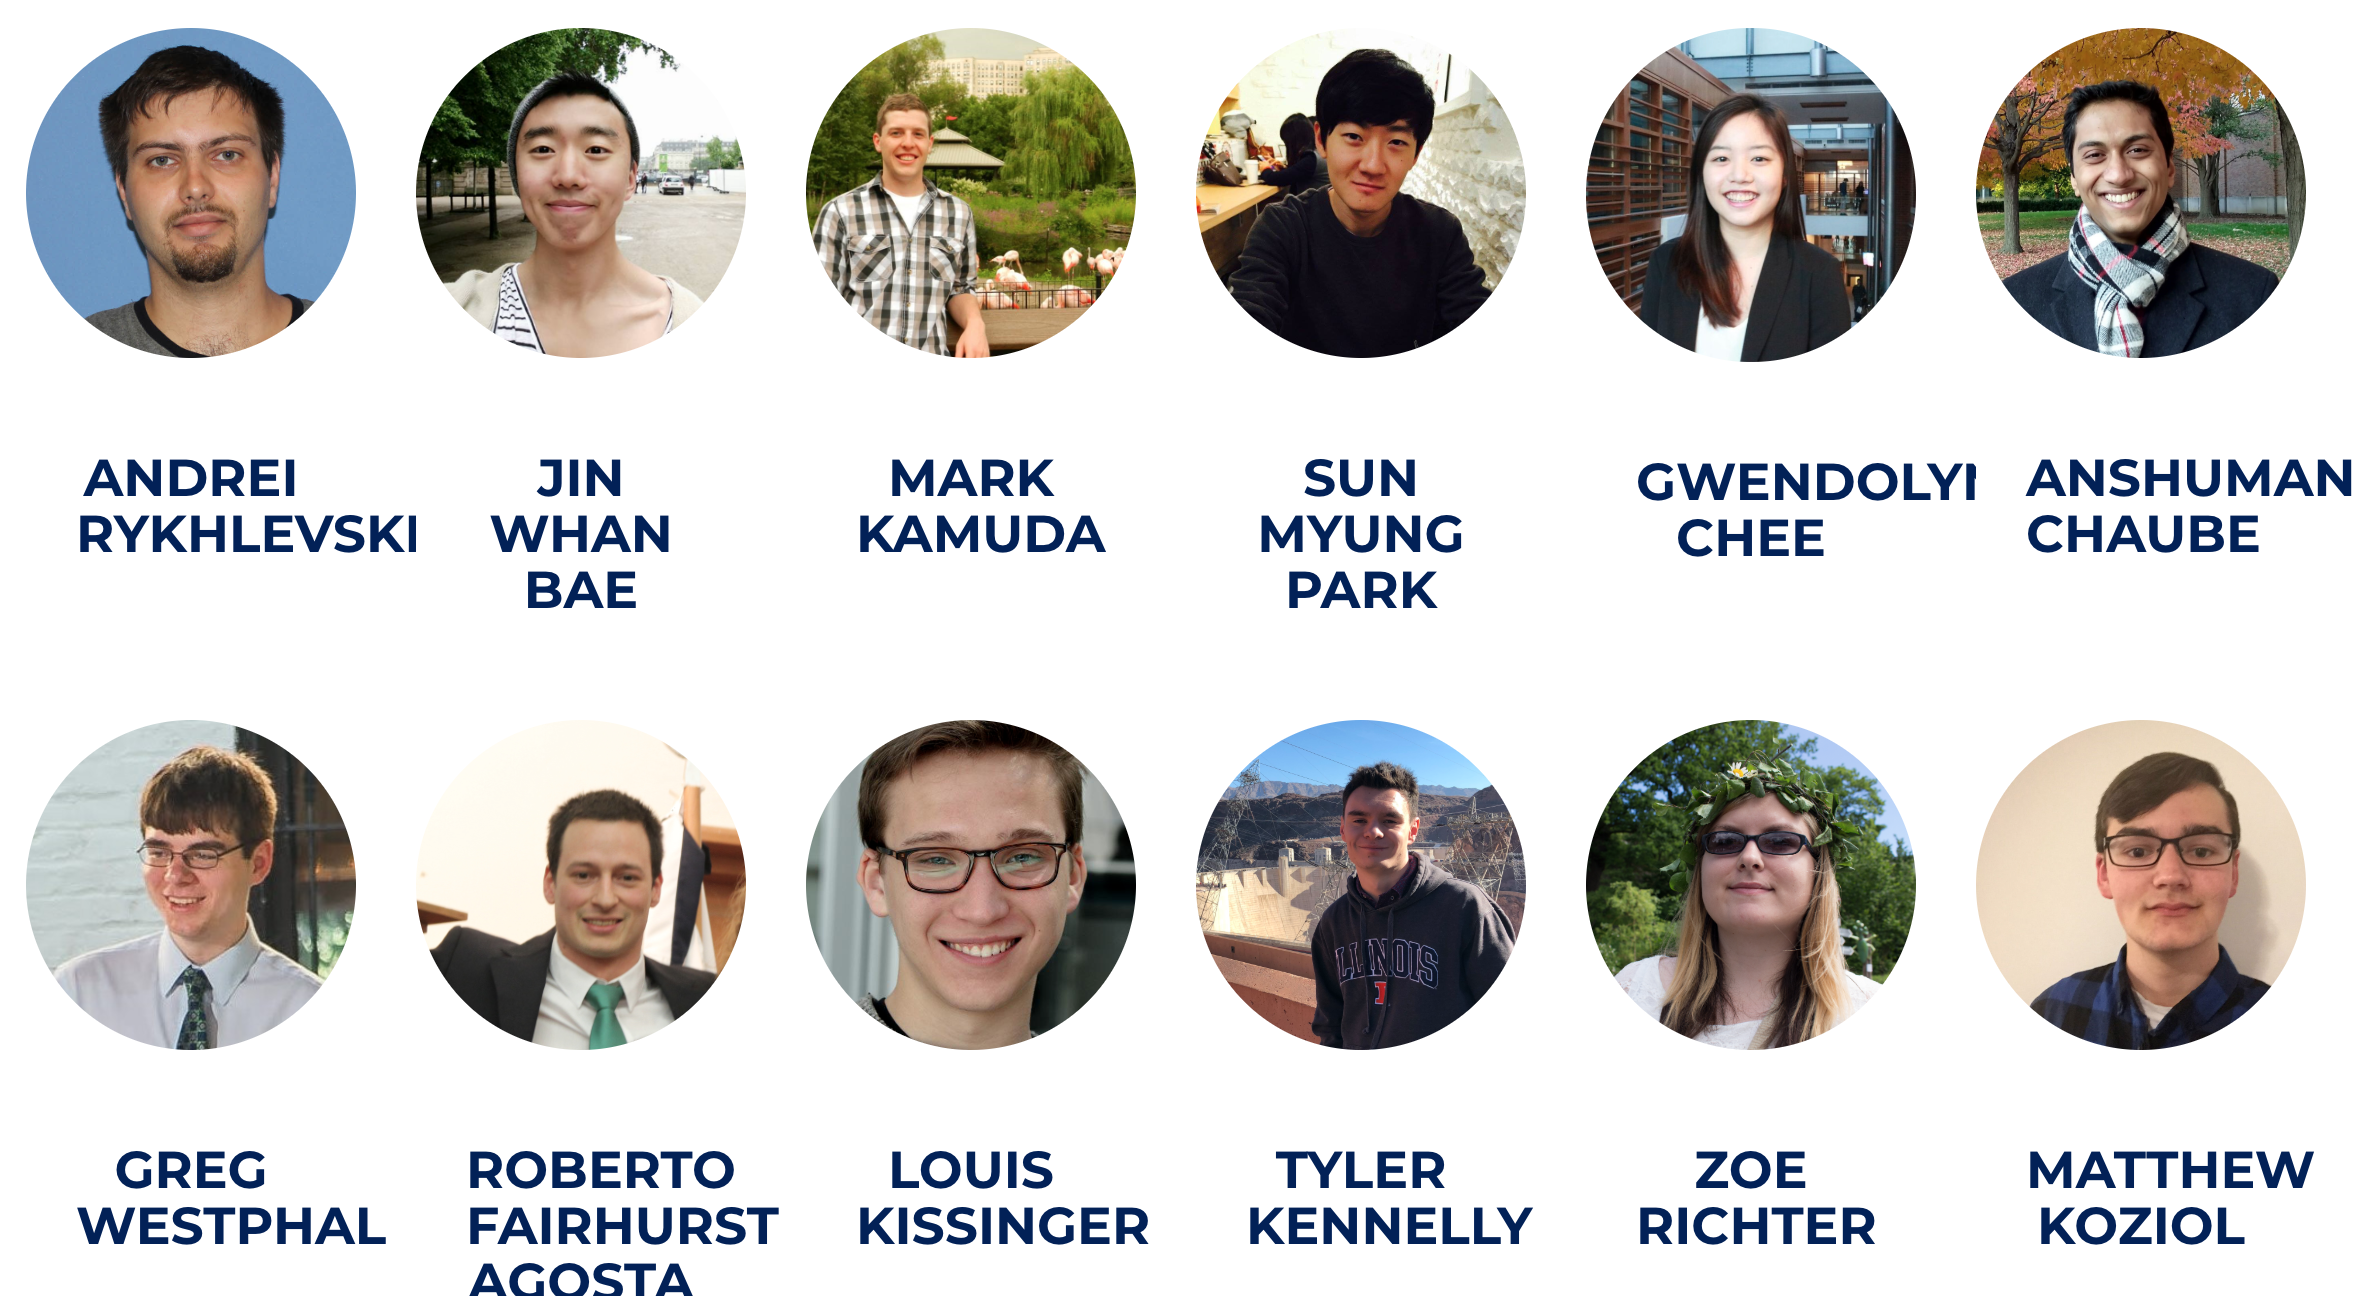
\includegraphics[height=0.71\textwidth]{./images/arfc1.png}
               \end{figure}            
\end{frame}

\begin{frame}
  \frametitle{Insights at Disparate Scales}
               \begin{figure}[t]
                \vspace*{-0.1in}
			\hspace*{-0.35in}
                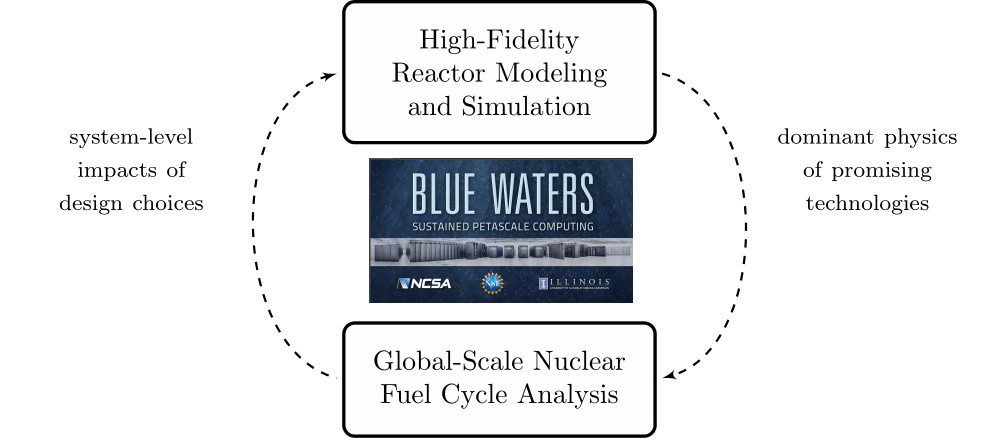
\includegraphics[height=0.5\textwidth]{./images/synergy.png}
               \end{figure}            
\end{frame}

\subsection{Fission basics}
\begin{frame}
  \frametitle{Nuclear Fission Reaction}
               \begin{figure}[t]
                \vspace*{-0.1in}
			\hspace*{-0.35in}
                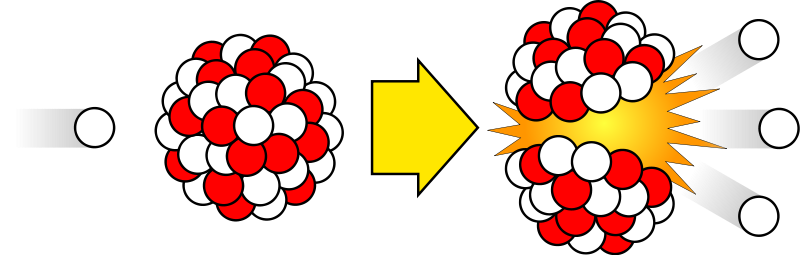
\includegraphics[height=0.25\textwidth]{./images/800px-Fission.png}
               \end{figure}            
\end{frame}

\begin{frame}
  \frametitle{Nuclear Fission Chain Reaction}
               \begin{figure}[t]
                \vspace*{-0.1in}
			\hspace*{-0.35in}
                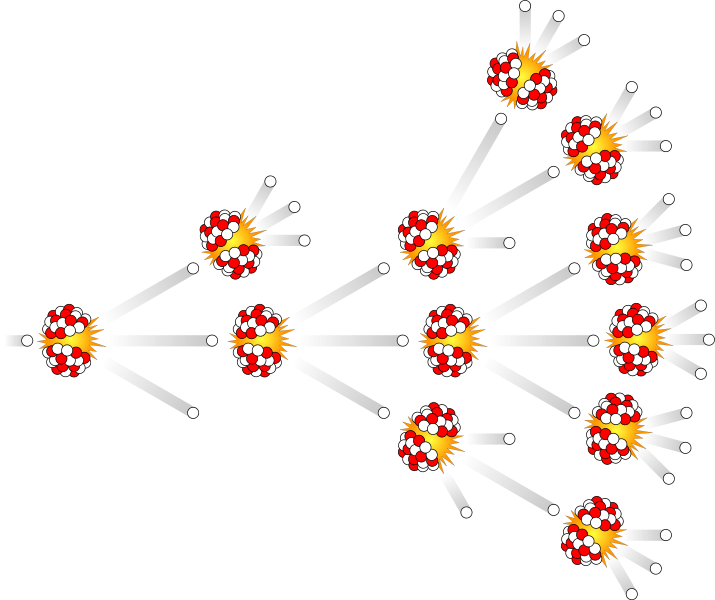
\includegraphics[height=0.7\textwidth]{./images/715px-Chainreaction.png}
               \end{figure}            
\end{frame}

\begin{frame}
  \frametitle{Nuclear Power Plant}
  \animategraphics[width=\textwidth,autoplay,loop]{6}{./images/gif/frame-}{0}{23}
\end{frame}

\subsection{Motivation}
\begin{frame}
  \frametitle{Why Molten Salt Reactors?}
                  \vspace*{-0.1in}
              \begin{block}{Main advantages of liquid-fueled \glspl{MSR} \cite{elsheikh_safety_2013}}
               \begin{enumerate}
                \item High coolant temperature (600-750$^{\circ}$C).
                \item Various fuels can be used ($^{235}$U, $^{233}$U, Thorium, U/Pu).
                \item Increased inherent safety.
                \item High fuel utilization $\Rightarrow$ less nuclear waste generated.
                \item Online reprocessing and refueling.
               \end{enumerate}
               \end{block}
                  \vspace*{-0.1in}               
               \begin{block}{Main advantages of \gls{MSBR} \cite{robertson_conceptual_1971}}
               \begin{enumerate}
                \item Produces more fissile material than it consumes (breeding ratio 1.06).
                \item Thorium cycle limits plutonium and minor actinides.
                \item Could transmute spent fuel from existing \gls{NPP}.
               \end{enumerate}
               \end{block}

\end{frame}

\begin{frame}
  \frametitle{Challenges in simulation \gls{MSR}}
                  \vspace*{-0.05in}
               \begin{enumerate}
                \item Contemporary burnup codes cannot treat fuel movement.
                \item Neutron precursor location is hard to estimate.
                \item Operational and safety parameters change during reactor operation.
                \item Power generation strongly depends on fuel temperature and vica versa.
               \end{enumerate}

           \begin{figure}[t]
                \vspace*{-0.3in}
			\hspace*{-0.2in}
                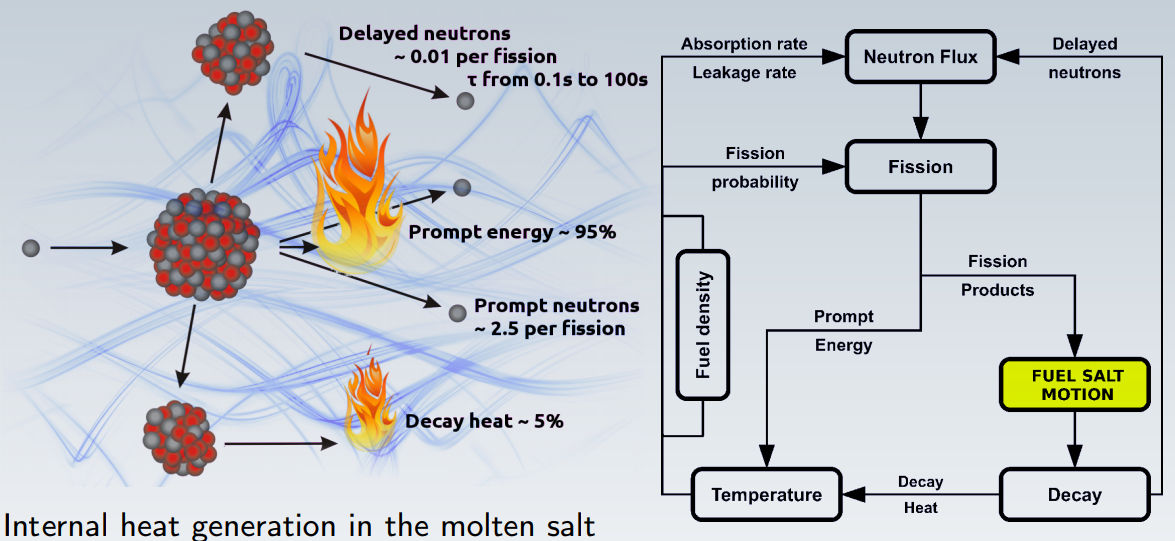
\includegraphics[height=0.5\textwidth]{./images/coupled_physics.png}
		\vspace*{-0.05in}
		\caption{Multiphysics simulation scheme for \gls{MSR} (Courtesy of Manuele Aufiero,2012).}
     	 \end{figure}               
\end{frame}

\begin{frame}
  \frametitle{Research objectives}
                  \vspace*{-0.1in}
              \begin{block}{Goal \#1: Tool for online reprocessing depletion simulation (SaltProc)\cite{rykhlevskii_saltproc}}
               \begin{enumerate}
                \item Create high-fidelity full-core neutronics model of MSBR.
                \item Develop online reprocessing simulation code, SaltProc, which expands the neutronics code capability for simulation liquid-fueled \gls{MSR} operation.
                \item Analyse \gls{MSBR} neutronics and fuel cycle performance.
               \end{enumerate}
               \end{block}

              \begin{block}{Goal \#2: Tool for multiphysics simulation of \gls{MSR} (Moltres)\cite{lindsay_introduction_2018}}
               \begin{enumerate}
                \item Demonstrate steady-state coupling of neutron fluxes, precursors, and thermal-hydraulics.
                \item Implement advective movement of delayed neutron precursors.
                \item Demonstrate capabilities with 2D axisymmetric and 3D mesh.
               \end{enumerate}
               \end{block}


              
\end{frame}

\section{Point Kinetics \& TH Coupling}
\subsection{Point and Multi-point Kinetics}
\begin{frame}
        \frametitle{PyRK: Python for Reactor Kinetics}

               \begin{figure}[t]
                \vspace*{-0.1in}
                
\includegraphics[height=0.5\textheight]{./images/pyrk.png}
                       \caption{Special purpose reactor kinetics python tool
                       (https://github.com/pyrk/pyrk) \cite{huff_pyrk:_2015}. 
                       Research software for simple PRKE: \emph{caveat emptor.}}
               \end{figure}

               \begin{itemize}
                       \item Multiple precursor groups ($j$ groups)
                       \item Multiple decay heat groups ($k$ groups)
                       \item Lumped Parameter thermal hydraulics model
                       \item Optional 1-D conduction in pebble fuel compacts
                       \item Object-oriented, geometry and material agnostic framework
               \end{itemize}
\end{frame}


%------------------------------------------------------------------------------------
\begin{frame}
        \frametitle{Point Reactor Kinetics}
        \begin{align}
    p &= \mbox{ reactor power }\\
    \rho(t,&T_{fuel},T_{cool},T_{mod}, T_{refl}) = \mbox{ reactivity}\\
    \beta &= \mbox{ fraction of neutrons that are delayed}\\
    \beta_j &= \mbox{ fraction of delayed neutrons from precursor group j}\\
    \zeta_j &= \mbox{ concentration of precursors of group j}\\
    \lambda_{d,j} &= \mbox{ decay constant of precursor group j}\\
    \Lambda &= \mbox{ mean generation time }\\
    \omega_k &= \mbox{ decay heat from FP group k}\\
    \kappa_k &= \mbox{ heat per fission for decay FP group k}\\
    \lambda_{FP,k} &= \mbox{ decay constant for decay FP group k}\\
    T_i &= \mbox{ temperature of component i}
\end{align}

\end{frame}

%------------------------------------------------------------------------------------
\begin{frame}
\frametitle{Point Reactor Kinetics}
\begin{equation}
\frac{d}{dt}\left[
    \begin{array}{c}
      p\\
      \zeta_1\\
      .\\
      \zeta_j\\
      .\\
      \zeta_J\\
      \omega_1\\
      .\\
      \omega_k\\
      .\\
      \omega_K\\
      T_{i}\\
      .\\
      T_{I}\\
    \end{array}
    \right]
    =
    \left[
      \begin{array}{ c }
        \frac{\rho(t,T_{i},\cdots)-\beta}{\Lambda}p +
        \displaystyle\sum^{j=J}_{j=1}\lambda_{d,j}\zeta_j\\
        \frac{\beta_1}{\Lambda} p - \lambda_{d,1}\zeta_1\\
        .\\
        \frac{\beta_j}{\Lambda}p-\lambda_{d,j}\zeta_j\\
        .\\
        \frac{\beta_J}{\Lambda}p-\lambda_{d,J}\zeta_J\\
        \kappa_1p - \lambda_{FP,1}\omega_1\\
        .\\
        \kappa_kp - \lambda_{FP,k}\omega_k\\
        .\\
        \kappa_{k p} - \lambda_{FP,k}\omega_{k}\\
        f_{i}(p, C_{p,i}, T_{i}, \cdots)\\
        .\\
        f_{I}(p, C_{p,I}, T_{I}, \cdots)\\
      \end{array}
      \right]
\end{equation}
\end{frame}

%------------------------------------------------------------------------------------
\begin{frame}
        \frametitle{Lumped Parameter Heat Transfer}

The heat flow out of body $i$ is the sum of surface heat flow by conduction,
convection, radiation, and other mechanisms to each adjacent body, $j$:
\begin{align}
Q &= Q_i + \sum_j Q_{ij}\\
  &=Q_i +  \sum_j\frac{T_{i} - T_{j}}{R_{th,ij}}\\
\dot{Q} &= \mbox{total heat flow out of body i }[J\cdot s^{-1}]\\
Q_i &= \mbox{other heat transfer, a constant }[J\cdot s^{-1}]\\
T_i &= \mbox{temperature of body i }[K]\\
T_j &= \mbox{temperature of body j }[K]\\
j &= \mbox{adjacent bodies }[-]\\
R_{th} &= \mbox{thermal resistence of the component }[K \cdot s \cdot J^{-1}].
\end{align}
\end{frame}

%------------------------------------------------------------------------------------
\begin{frame}
        \frametitle{PB-FHR Example}

               \begin{figure}[t]
                \vspace*{-0.1in}
                       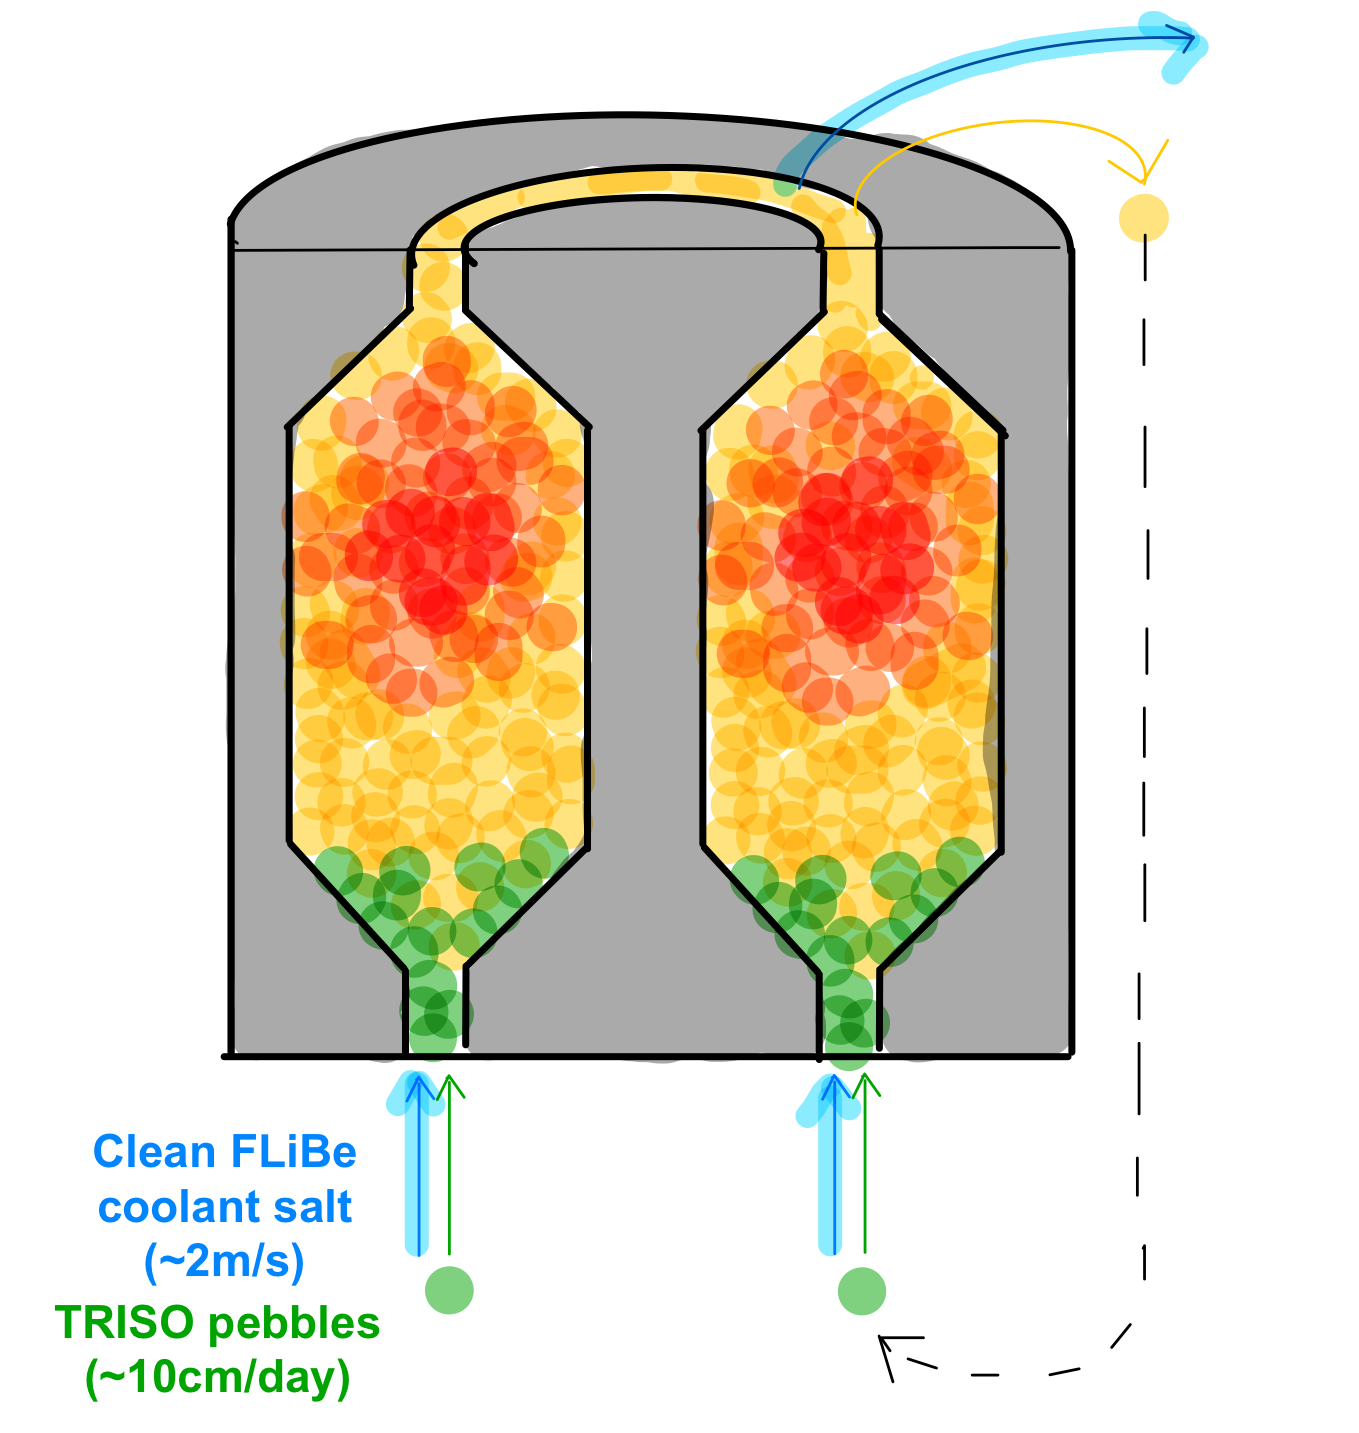
\includegraphics[height=0.5\textwidth]{./images/pbfhr-fuel-movement.png}
                       \caption{The pebble fuel can be assumed approximately 
                       stationary, as their movement is not comparable to the 
                       longest precursor decay times.}
               \end{figure}

\end{frame}


%------------------------------------------------------------------------------------
\begin{frame}
        \frametitle{Point Reactor Kinetics}

               \begin{figure}[t]
                \vspace*{-0.1in}
                       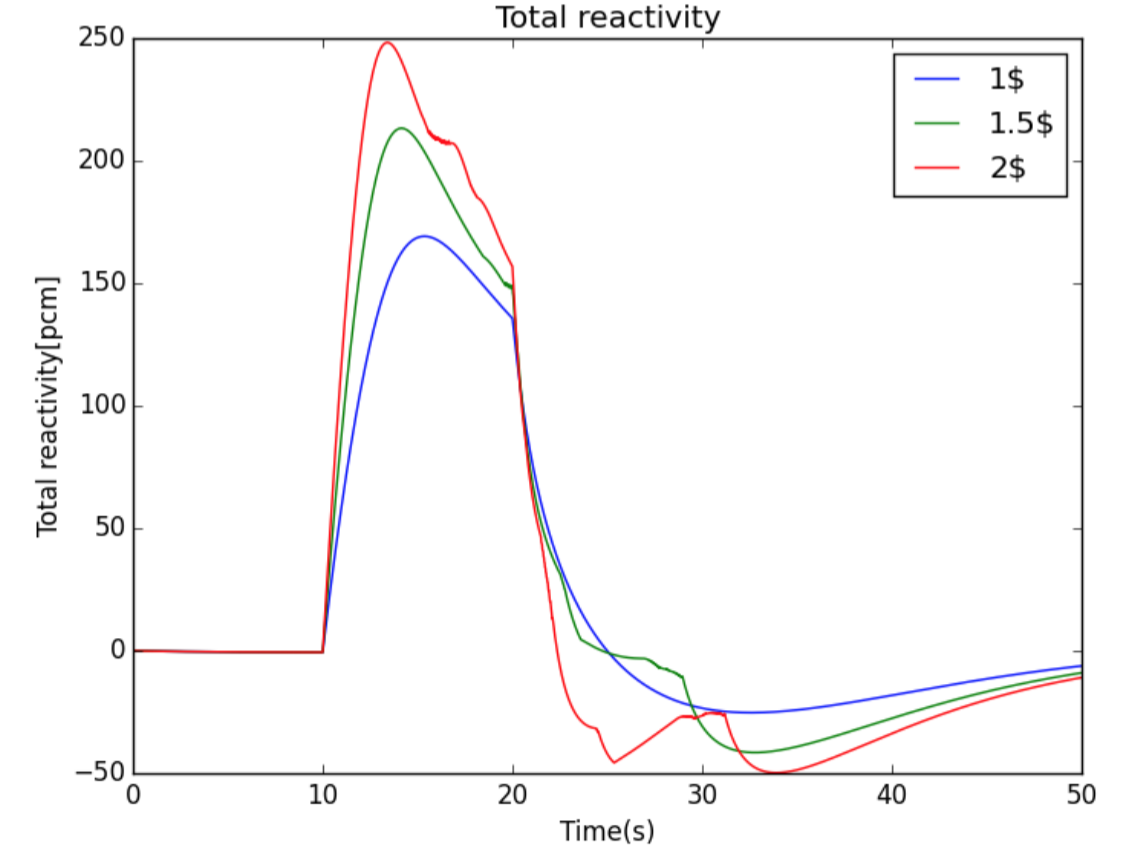
\includegraphics[height=0.5\textwidth]{./images/pbfhr-total-reactivity.png}
                       \caption{Total reactivity during ramped reactivity 
                       insertion as a function of inserted reactivity
                       \cite{wang_coupled_2016}.}
               \end{figure}

\end{frame}



%------------------------------------------------------------------------------------
\begin{frame}
        \frametitle{PB-FHR Example}

               \begin{figure}[t]
                \vspace*{-0.1in}
                       \hspace*{-0.3in}
                       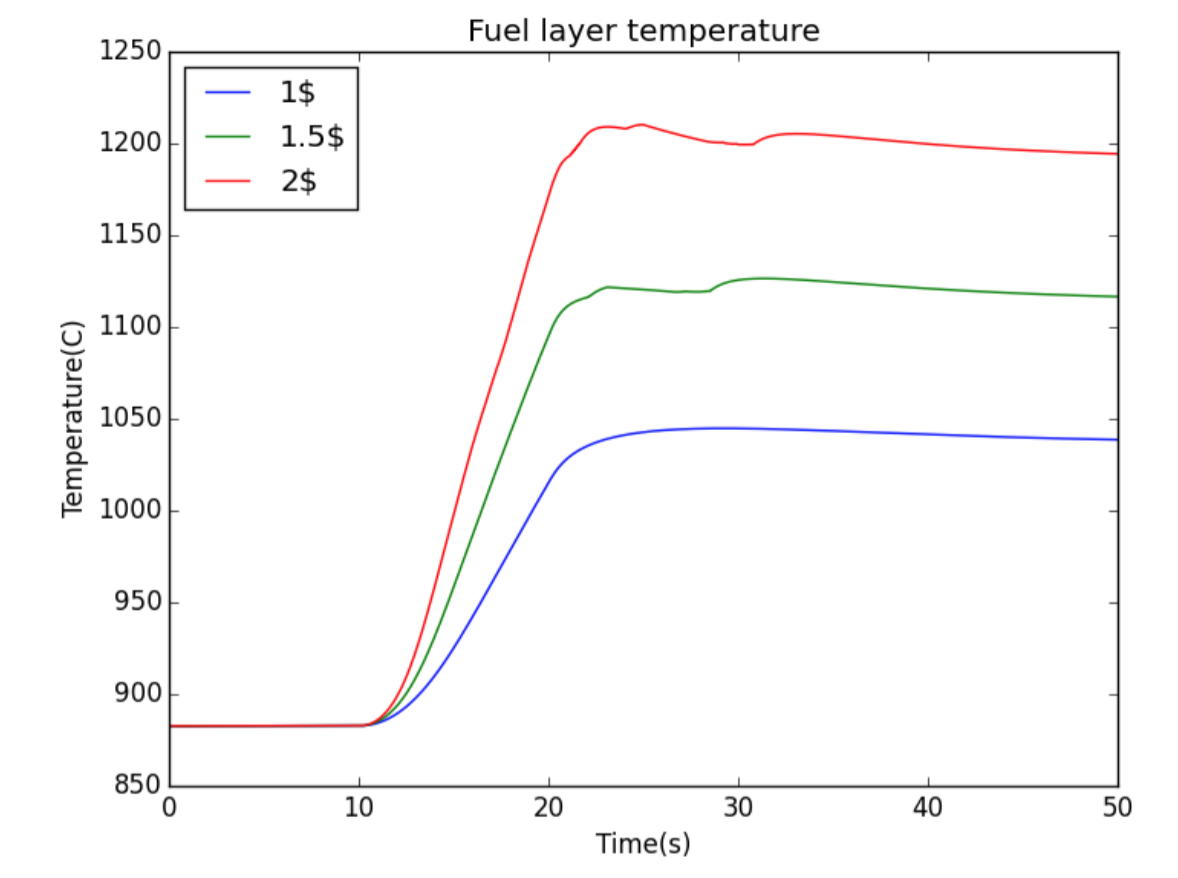
\includegraphics[height=0.3\textwidth]{./images/pbfhr-fuel-temp.png}
                       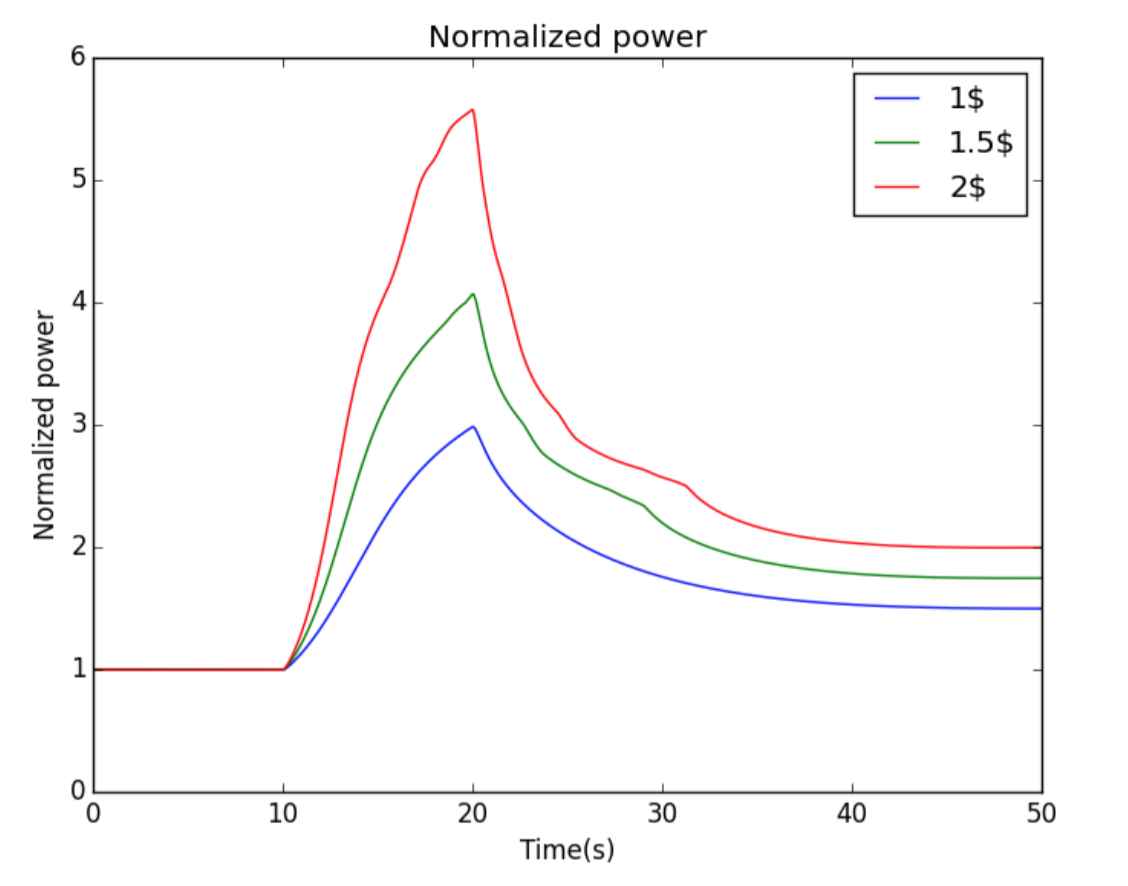
\includegraphics[height=0.3\textwidth]{./images/pbfhr-avg-pow.png}
                       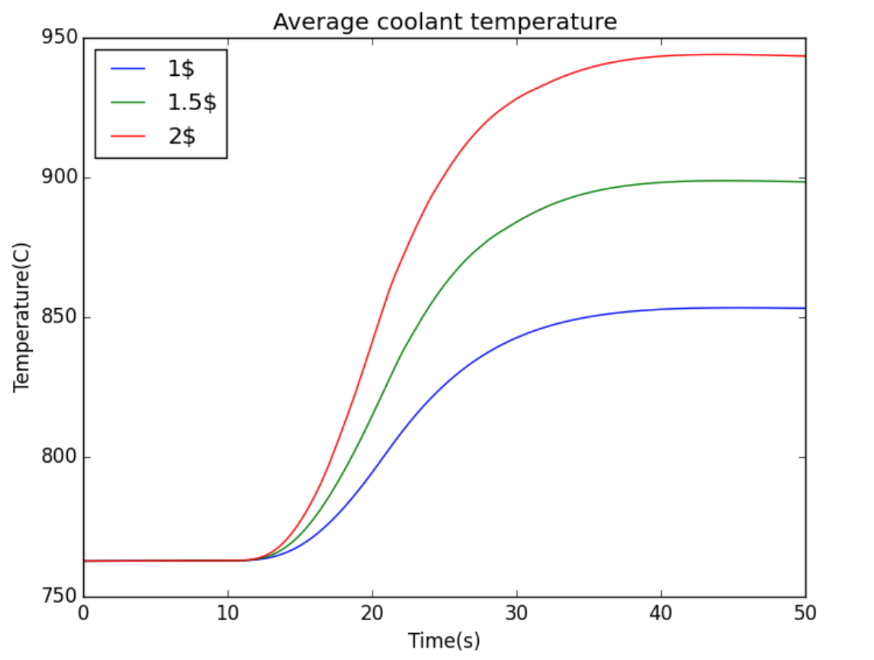
\includegraphics[height=0.3\textwidth]{./images/pbfhr-coolant-temp.png}
                       \caption{Average fuel temperature (left) and average 
                       normalized core power (right) during a ramp reactivity 
                       insertion in the PB-FHR \cite{wang_coupled_2016}.}
               \end{figure}

\end{frame}


%------------------------------------------------------------------------------------
\begin{frame}
        \frametitle{Point Reactor Kinetics}

               \begin{figure}[t]
                \vspace*{-0.1in}
                       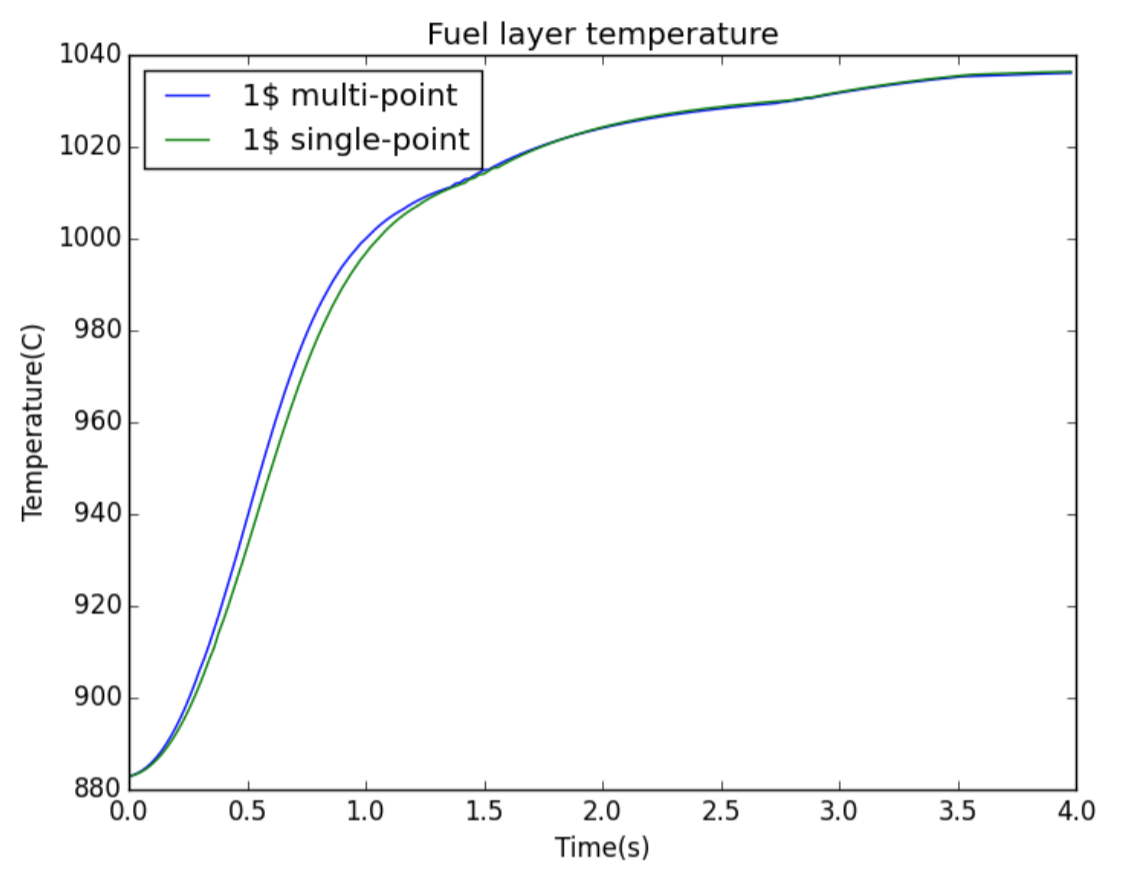
\includegraphics[height=0.5\textwidth]{./images/pbfhr-multi-single-point.png}
                       \caption{Fuel temperature rise following 1\$ ramp 
                       reactivity insertion, calculated with multipoint and 
                       single point kinetics in PyRK \cite{wang_coupled_2016}.}
               \end{figure}

\end{frame}

\section{Spatial Kinetics \& TH Coupling with Precursor Advection}

\begin{frame}
  \frametitle{Full-core SERPENT model of \gls{MSBR}}
    \begin{figure}[t]
                \vspace*{-0.2in}
                   \hspace*{-0.39in}
                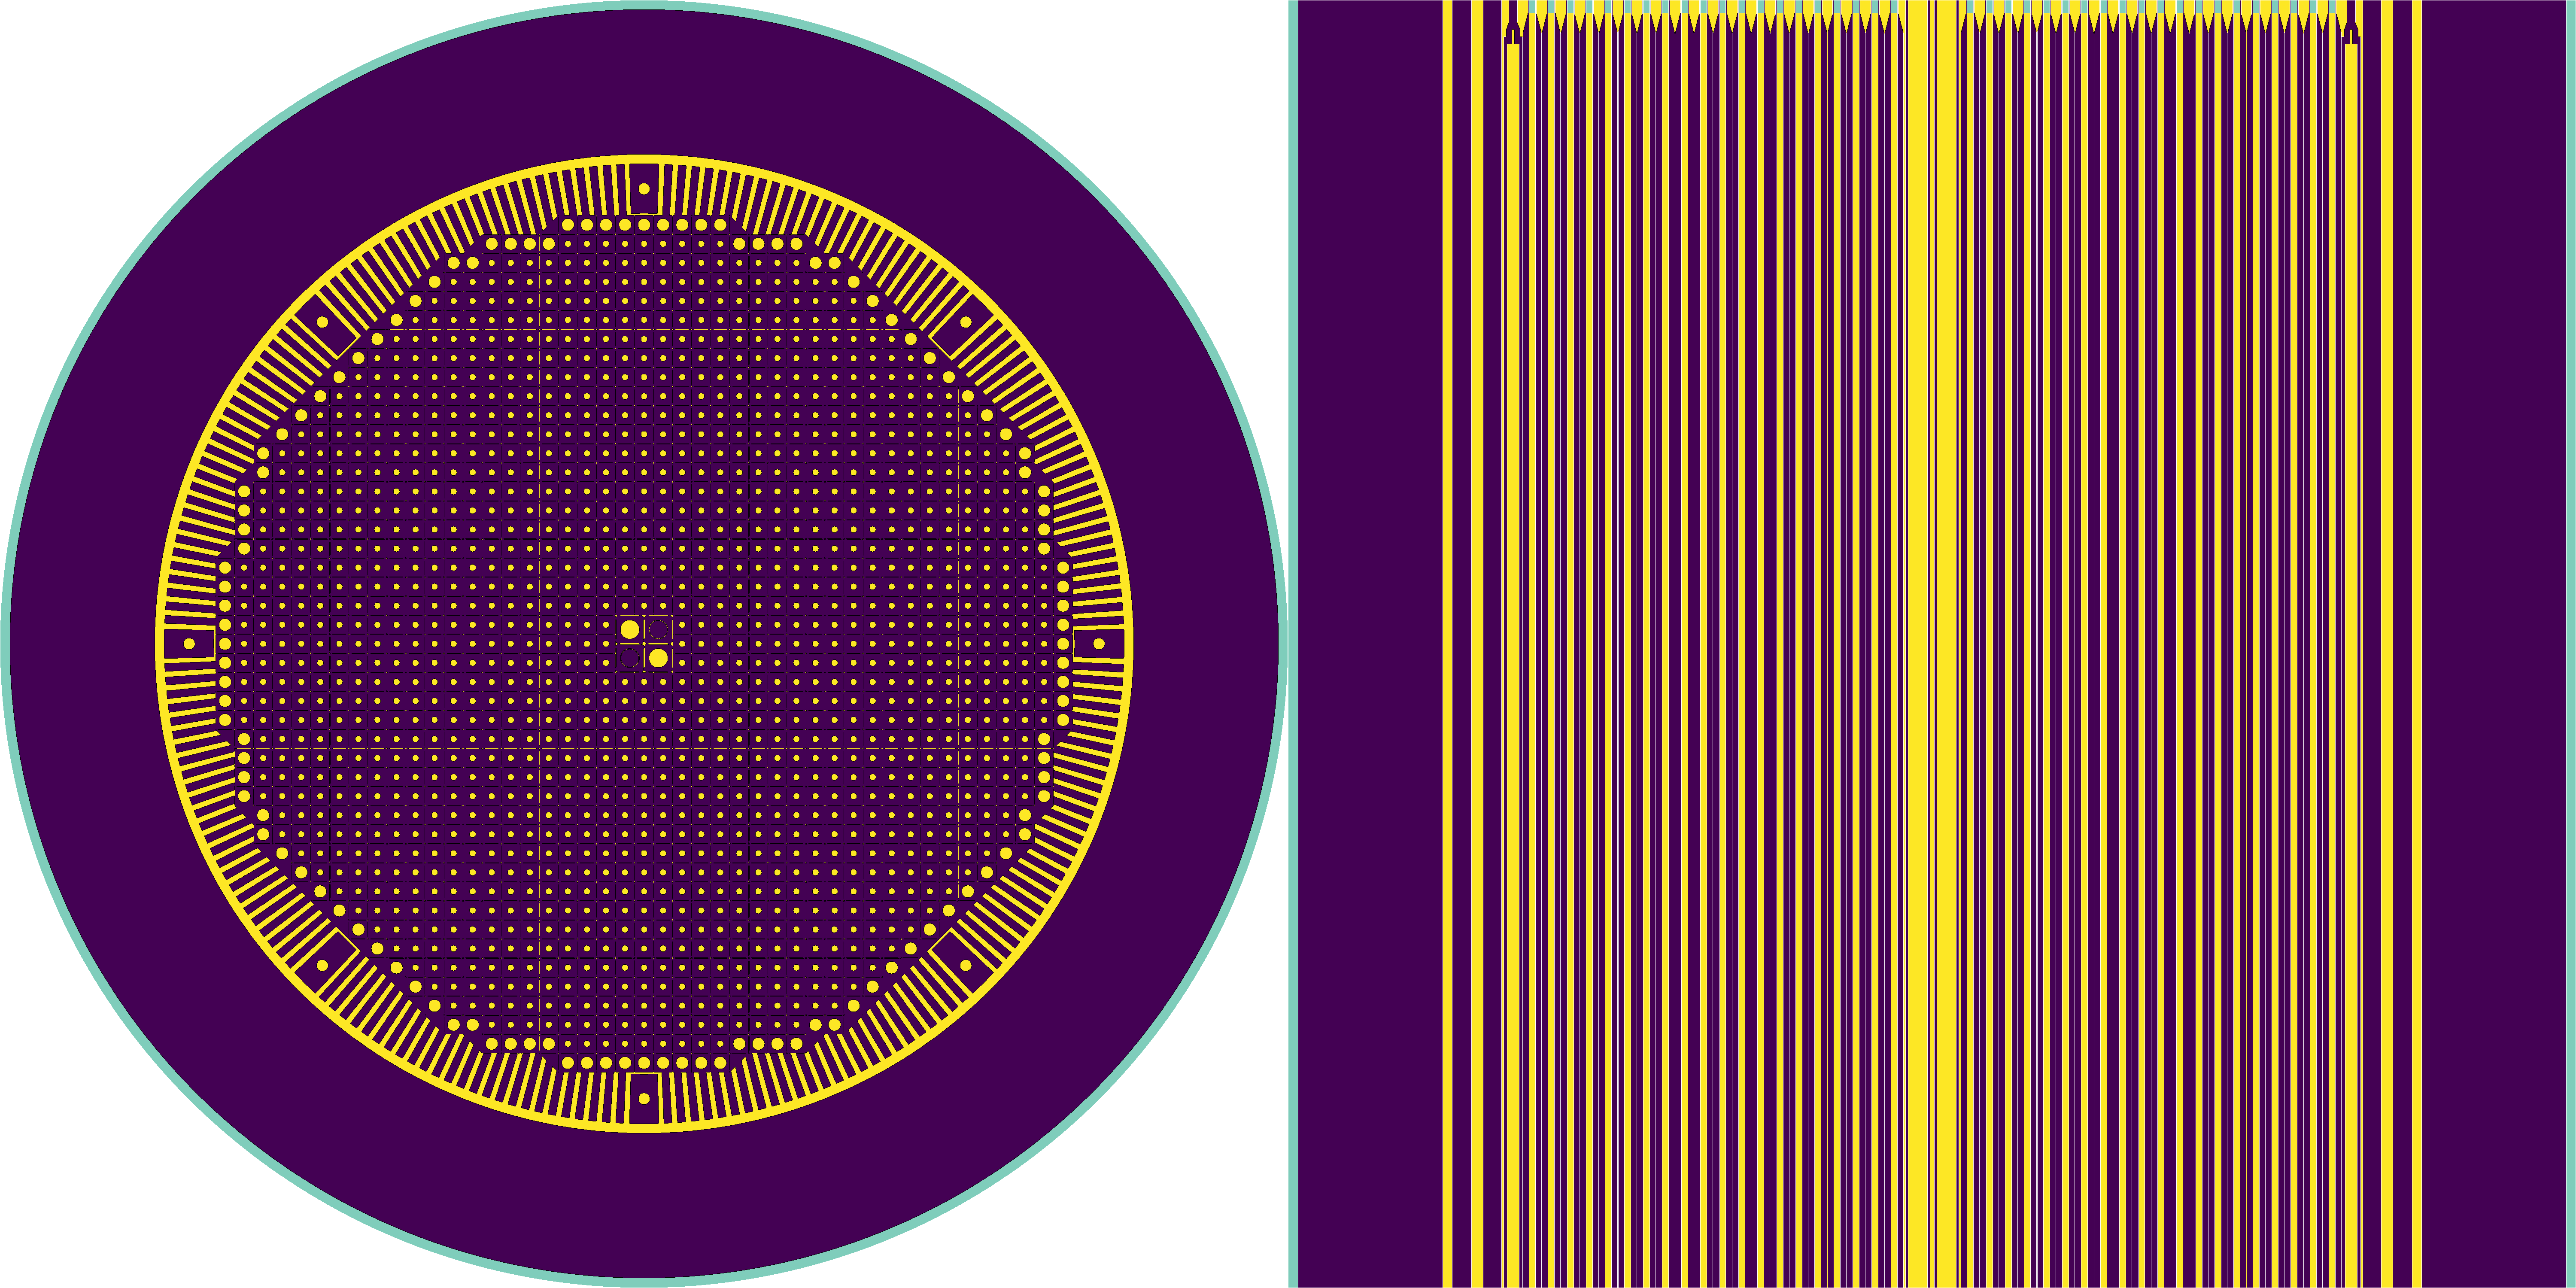
\includegraphics[height=0.6\textwidth]{./images/geometry_main_views.png}
                \caption{Plan (left) and elevation (right) view of MSBR model.}
      \end{figure}
     
\end{frame}

\begin{frame}
  \frametitle{Core Zone II}
  \begin{figure}[t]
     \vspace{-0.25in}
       \hspace*{-0.43in}
       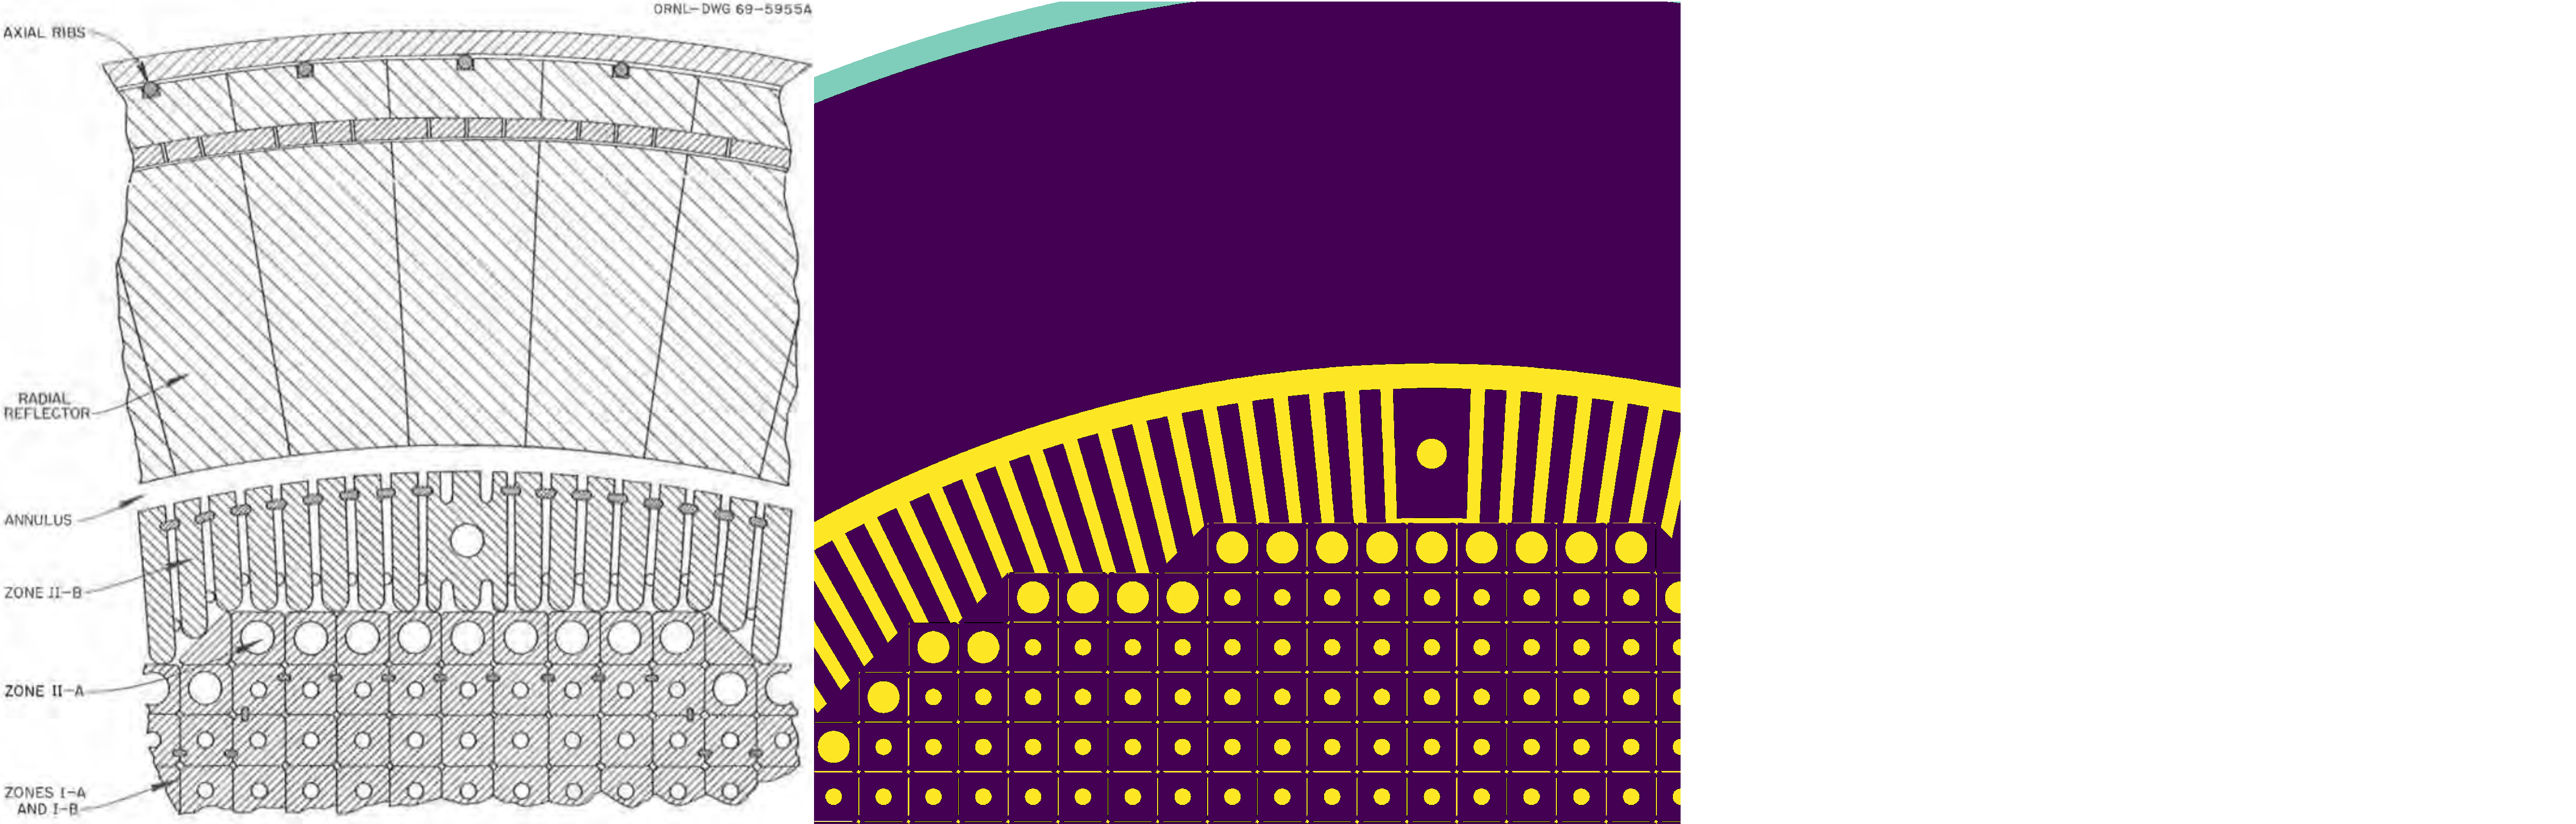
\includegraphics[height=0.77\textheight]{./images/reflector_and_elements.png}
            \caption{Detailed plan view of graphite reflector and moderator elements.}
  \end{figure}
           \vspace{-0.1in}
\end{frame}

\begin{frame}
  \frametitle{Moderator element geometry (Zone I)}
    \begin{figure}[t]
                \vspace*{-0.2in}
                   \hspace*{-0.37in}
                \includegraphics[height=0.60\textwidth]{./images/zone_I_mesh.png}
                \vspace*{-0.05in}
                \caption{Molten Salt Breeder Reactor Zone I unit cell geometry from the reference \cite{robertson_conceptual_1971} (left) and SERPENT 2 (right).}
      \end{figure}
     
\end{frame}



\begin{frame}
\frametitle{Online reprocessing method}
  \begin{columns}
    \column[t]{6cm}
	\begin{figure}[t]
                \vspace*{-0.35in}
			\hspace{-0.3in}
                 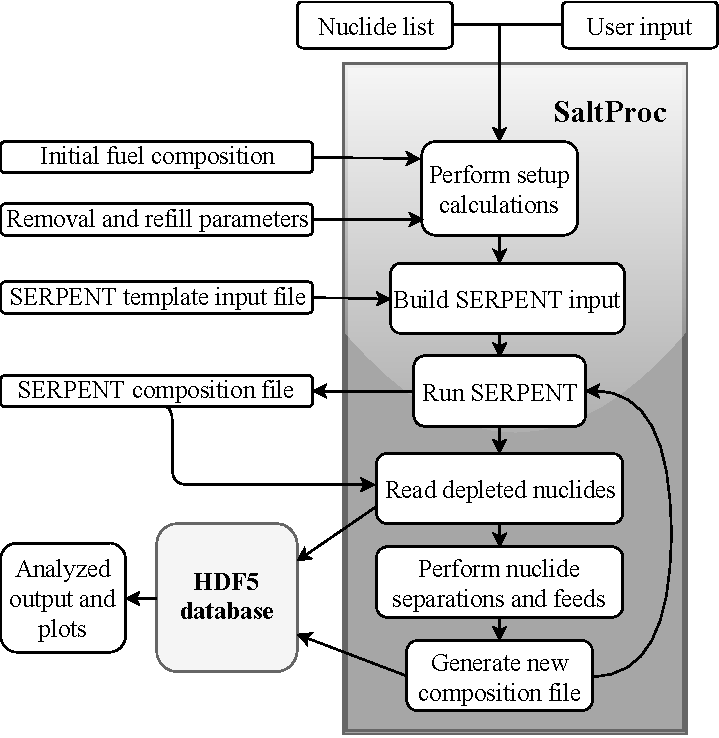
\includegraphics[height=\textwidth]{./images/saltproc_flowchart.pdf}
                \vspace*{-0.05in}
                \caption{Flow chart for the SaltProc.}
      \end{figure}

    \column[t]{6cm}
             \begin{block}{SaltProc capabilities}
               \begin{itemize}             
               \item Remove specific isotopes from the core with specific parameters (reprocessing interval, mass rate, removal efficiency)
               \item Add specific isotopes into the core
               \item Maintain constant number density of specific isotope in the core
	       \item Store stream vectors in an HDF5 database for further analysis or plots
	       \item Generic geometry: an infinite medium, a unit cell, a multi-zone simplified assembly, or a full-core
               \end{itemize}
               \end{block}
  \end{columns}
\end{frame}

\begin{frame}
  \frametitle{Online reprocessing method}
     \begin{figure}[t]
                \vspace*{-0.1in}
                  % \hspace*{-0.37in}
                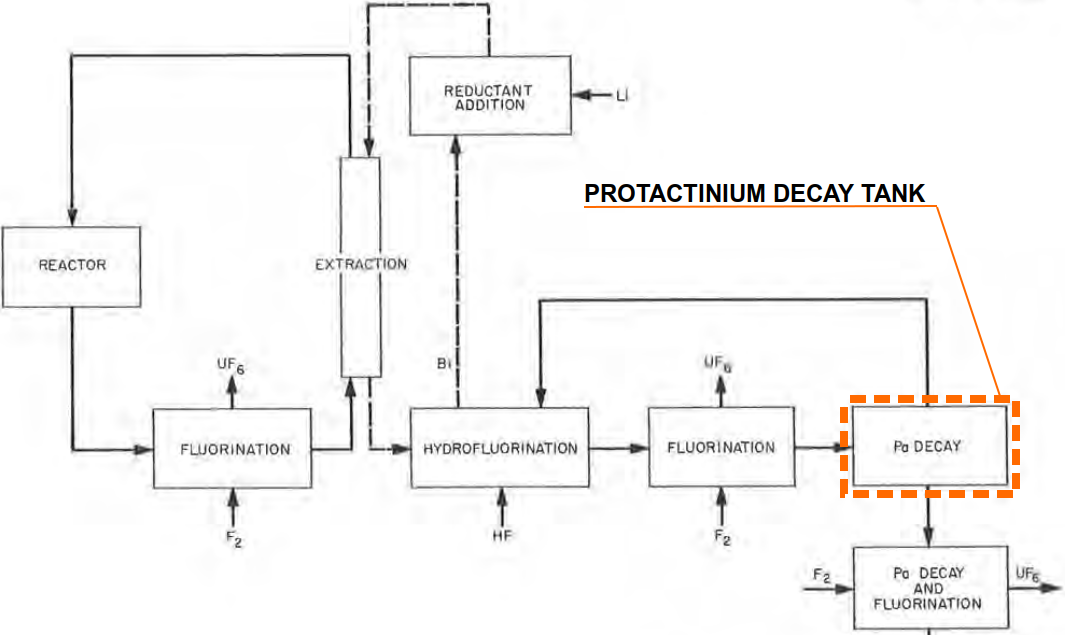
\includegraphics[height=0.45\textwidth]{./images/pa_isolation.png}
                \vspace*{-0.09in}
                \caption{Protactinium isolation with uranium removal by fluorination \cite{robertson_conceptual_1971}.}
      \end{figure}
                      \vspace*{-0.22in}
             \begin{block}{Online reprocessing approach}
               \begin{itemize}             
               \item Continuously removes all poisons, noble metals, and gases.
               \item $^{233}$Pa is continuously removed from the fuel salt into a decay tank.
               \end{itemize}
               \end{block}
               \vspace{-0.05in}
$\qquad\qquad\qquad\qquad^{232}_{90}$Th+$^1_0$n$\rightarrow^{233}_{90}$Th$\xrightarrow[\text{22.3 min}]{\beta^-}$ $^{233}_{91}$Pa$\xrightarrow[\text{26.967 d}]{\beta^-}$ $^{233}_{92}$U
\end{frame}


\subsection{EU Nuclear Operation until 2050}

\begin{frame}
	\frametitle{Historical Operation of EU Reactors}

\begin{table}[h]
	\centering
	\scalebox{0.86}{
		\begin{tabular}{cccc}
			\hline
			\textbf{Category } & \textbf{Value} & \textbf{Unit} & \textbf{Specifics}\\ \hline
			Total UOX Usage  & 176,600 & MTHM &  \\ 
			Total MOX Usage  & 6,953 & MTHM & \\ 
			Total Used UOX Stored  & 110,013 & MTHM & \gls{UNF} that is not reprocessed\\  
			Total Used UOX Stored (France) & 12,943 & MTHM & \gls{UNF} that is not reprocessed \\
			Total Tails  & 1,059,210 & MTHM & \\ 
			Total Natural U Used  & 1,235,810 & MTHM & \\ \hline
		\end{tabular}}
		\caption{Simulation Results for Historical Nuclear Operation 
		of \gls{EU} Nations}
		\label{tab:sim_result}
\end {table}

\end{frame}

\begin{frame}
	\frametitle{Tails and UNF Inventory}
\begin{figure}[htbp!]
\begin{minipage}[b]{.45\linewidth}
	\begin{center}
		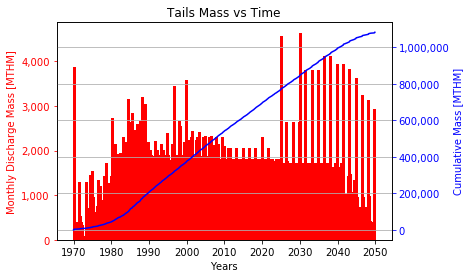
\includegraphics[width=\textwidth]{./images/eu_future/tails.png}
	\end{center}
	\caption{Timeseries of Tails Mass in the \gls{EU}.}
	\label{fig:eu_tail}
\end{minipage}
\hspace{.5cm}
\begin{minipage}[b]{.45\linewidth}
	\centering
	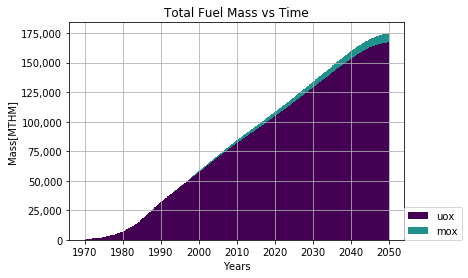
\includegraphics[width=\textwidth]{./images/eu_future/total_fuel.png}
	\caption{Timeseries of Total Fuel Usage in \gls{EU}.}
	\label{fig:eu_fuel}
\end{minipage}
\end{figure}
\end{frame}

\begin{frame}

\begin{figure}[htbp!]
	\begin{center}
			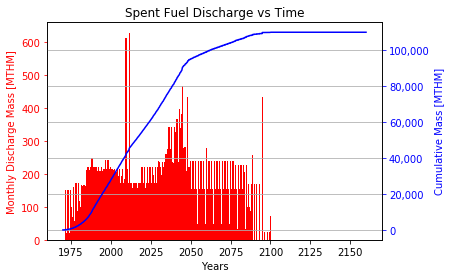
\includegraphics[scale=0.7]{./images/eu_future/snf_discharge.png}
	\end{center}
	\caption{Timeseries of Used Nuclear Fuel in \gls{EU}.}
	\label{fig:eu_snf}
\end{figure}

\end{frame}

\subsection{French Transition Scenario ~2160}

\begin{frame}
	\frametitle{SFR Deployment with Legacy UNF}
	\begin{itemize}
		\item Reprocessing UNF from all EU nations can start approx. 202 SFRs.
		\item Two generations of 66GWe SFRs = 220 SFRs
		\item Breeding Ratio of SFRs over one. ($\frac{23.95}{22.0} = 1.088$)
		\item Initial Pu loading of $4.9$ tons for ASTRID-type SFR \cite{varaine_pre-conceptual_2012}.
		\item $\frac{Pu \ from \ legacy \ \gls{UNF}}{4.9} \approx 202$
	\end{itemize}
\end{frame}

\begin{frame}
	\frametitle{Frech Transition Results}
	
\begin{table}[h]
	\centering
	\scalebox{0.86}{
		\begin{tabular}{ccc}
			\hline
			\textbf{Category} & \textbf{Unit} & \textbf{Value}  \\ \hline
			Total MOX used & MTHM & 63,820  \\ 
			Total \glspl{SFR} Deployed & & 220 \\ 
			Total Plutonium Reprocessed & MTHM & 15,099 \\ 
			Total \gls{ASTRID} fuel from UOX Waste & MTHM & 2,923  \\ 
			Total \gls{ASTRID} fuel from MOX Waste & MTHM  & 60,535 \\ 
			Total Tails used & MTHM & 49,779 \\ 
			Total legacy UNF reprocessed & MTHM & 54,111 \\ 
			Total Reprocessed Uranium Stockpile & MTHM & 183,740 \\ 
			Total Raffinate & MTHM & 33,806 \\ \hline
		\end{tabular}}
		\caption {\gls{SFR} Simulation Results}
		\label{tab:sfr_sim_result}
\end{table}

\end{frame}

\begin{frame}
	\frametitle{Material Flow in French Transition Scenario}
	
\begin{figure}[htbp!]
\begin{minipage}[b]{.45\linewidth}
	\begin{center}
		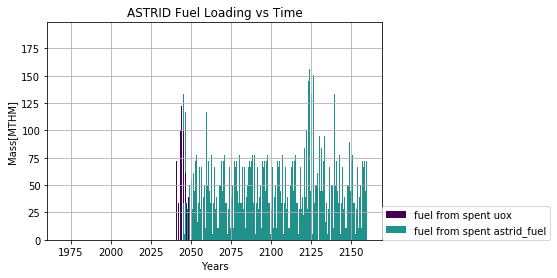
\includegraphics[width=\textwidth]{./images/french-transition/where_fuel.png}
	\end{center}
	\caption{Timeseries of fuel loaded into \glspl{SFR}, separated by origin}
	\label{fig:fuel}
\end{minipage}
\hspace{.5cm}
\begin{minipage}[b]{.45\linewidth}
	\centering
		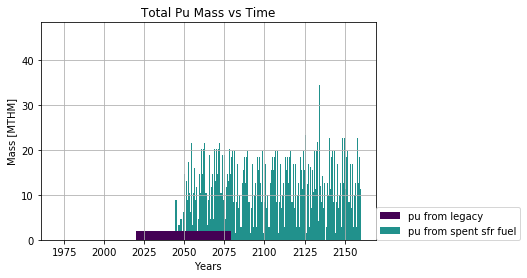
\includegraphics[width=\linewidth]{./images/french-transition/pu.png}
	\caption{Separated plutonium discharge from Reprocessing Plant}
	\label{fig:pu_no_cum}
\end{minipage}
\end{figure}

\end{frame}

\begin{frame}
	\frametitle{Material Flow in French Transition Scenario}
	
\begin{figure}[htbp!]
\begin{minipage}[b]{.45\linewidth}
	\begin{center}
		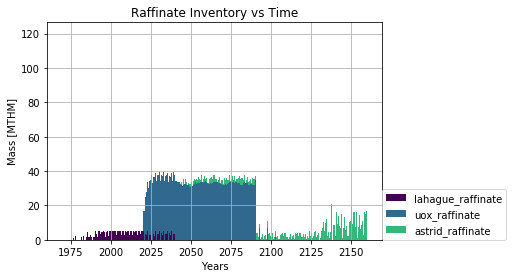
\includegraphics[width=\textwidth]{./images/french-transition/raffinate.png}
	\end{center}
	\caption{Timeseries of raffinate discharge from reprocessing plants}
	\label{fig:fuel}
\end{minipage}
\hspace{.5cm}
\begin{minipage}[b]{.45\linewidth}
	\centering
		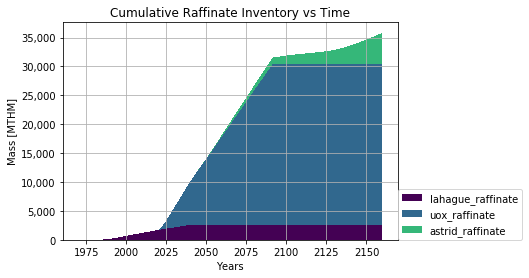
\includegraphics[width=\linewidth]{./images/french-transition/raffinate_cum.png}
	\caption{Cumulative raffinate inventory separated by origin}
	\label{fig:pu_no_cum}
\end{minipage}
\end{figure}

\end{frame}
\begin{frame}
  \frametitle{MOOSE Framework}
  \begin{columns}
    \column[t]{6cm}
  \begin{figure}[t]
       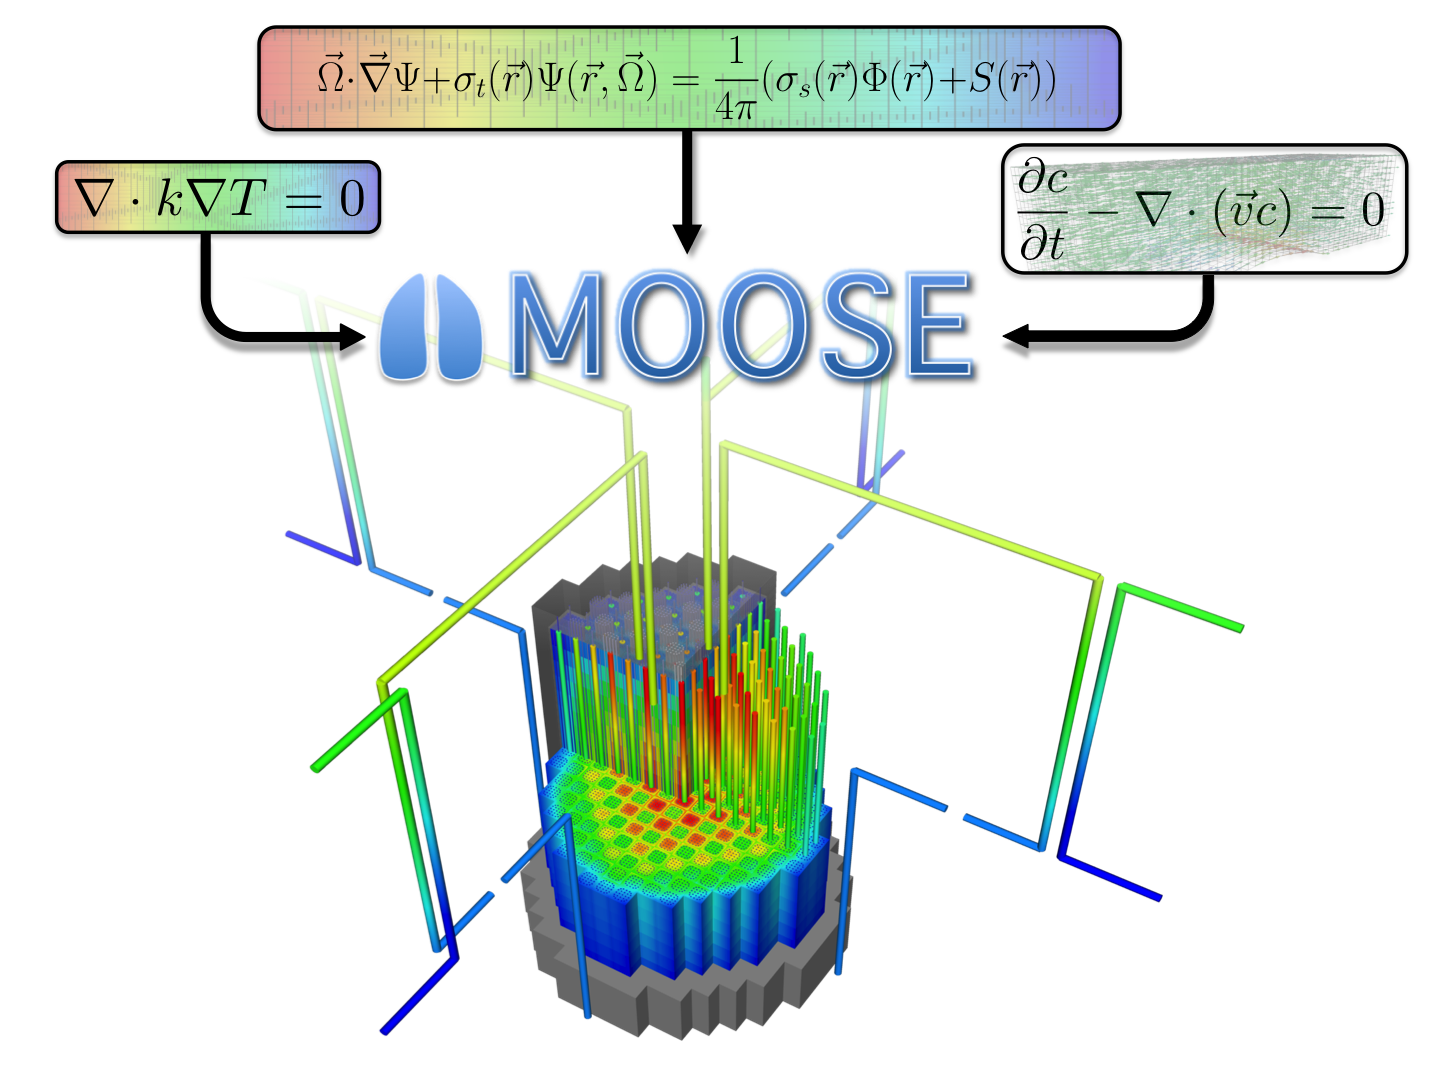
\includegraphics[width=\linewidth]{./images/moose.png}
            \caption{Multi-physics Object-Oriented Simulation Environment (MOOSE).}
  \end{figure}
	\column[t]{6cm}
               \begin{itemize}
               \item From Idaho National Lab (Gaston et al.  \cite{gaston_parallel_2009})
	       \item Fully-coupled, fully-implicit multiphysics solver
               \item MOOSE interfaces with libMesh to discretize simulation volume into finite elements
               \item Residuals and Jacobians handed off to PetSc which handles solution of resulting non-linear system of algebraic equations
	       \item Automatically parallel (largest runs \textgreater 100,000 CPU cores!)
	       \item Built-in mesh adaptivity
	       \item Intuitive parallel multiscale solves
               \end{itemize}

  \end{columns}
\end{frame}

\begin{frame}
        \frametitle{Moltres (Coupling in MOOSE)}
        \begin{center}
  \begin{figure}
   \vspace{-0.05in}
   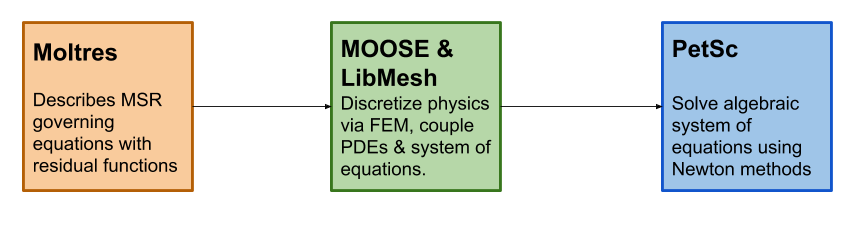
\includegraphics[width=1.1\textwidth]{./images/moltres-moose-diag.png}
    \end{figure}
        \end{center}
\end{frame}

\begin{frame}
        \frametitle{Intro to Moltres}
        \begin{itemize}  
                \item Fluid-fuelled, molten salt reactors
                \item Multi-group diffusion (arbitrary groups)
                \item Advective movement of delayed neutron precursors
                \item Navier-Stokes thermal hydraulics
                \item 3D unstructured
                \item 2D axisymmetric
                \item 3D structured 
                \item Initial developer: Alexander Lindsay \cite{lindsay_introduction_2018}
                \item Continued use and development ongoing at UIUC.
        \end{itemize}
\end{frame}


\begin{frame}
        \frametitle{Acquiring Moltres}
             \texttt{git clone https://github.com/arfc/moltres}\\
        \texttt{cd moltres}\\
        \texttt{git submodule init}\\
        \texttt{git submodule update}\\
\end{frame}

\begin{frame}
        \frametitle{Diffusion in Moltres}
        \footnotesize{
        \begin{align}
        \frac{1}{v_g}\frac{\partial \phi_g}{\partial t} &- \nabla \cdot D_g
        \nabla \phi_g + \Sigma_g^r \phi_g =\\
                &\sum_{g \ne g'}^G \Sigma_{g'\rightarrow g}^s \phi_{g'} + \chi_g^p \sum_{g' = 1}^G (1 -
        \beta) \nu \Sigma_{g'}^f \phi_{g'} + \chi_g^d \sum_i^I \lambda_i C_i
        \end{align}}
\begin{columns}
    \begin{column}{0.48\textwidth}
        \footnotesize{
        \begin{align*}
                v_g &= \mbox{speed of neutrons in group g} \\
                \phi_g &= \mbox{flux of neutrons in group g} \\
                t &= \mbox{time} \\
                D_g &= \mbox{Diffusion coefficient for neutrons in group g} \\
                \Sigma_g^r &= \mbox{macroscopic cross-section for}\\
                &\mbox{removal of neutrons from group g} \\
                \Sigma_{g'\rightarrow g}^s &= \mbox{macroscopic cross-section 
                of}\\
                &\mbox{  scattering from g' to g} \\
                \chi_g^p &= \mbox{prompt fission spectrum, neutrons in group g} \\
        \end{align*}}
    \end{column}
    \begin{column}{0.48\textwidth}
        %Content
        \footnotesize{
        \begin{align*}
                G &= \mbox{number of discrete groups, g} \\
                \nu &= \mbox{neutrons produced per fission} \\
                \Sigma_g^f &= \mbox{macroscopic fission cross section}\\
                &\mbox{ due to neutrons in group g} \\
                \chi_g^d &= \mbox{delayed neutrons in group g} \\
                I &= \mbox{ delayed neutron precursor groups} \\
                \beta &= \mbox{delayed neutron fraction}\\
                \lambda_i &= \mbox{average decay constant}\\
                &\mbox{of delayed neutron precursors in group i} \\
                C_i &= \mbox{concentration of delayed neutron}\\
                &\mbox{precursors in precursor group i}\\.
        \end{align*}}
    \end{column}
\end{columns}
\end{frame}

\begin{frame}
        \frametitle{Moltres Delayed Neutrons}
        \begin{align}
        \frac{\partial C_i}{\partial t} &= \sum_{g'= 1}^G \beta_i \nu
        \Sigma_{g'}^f \phi_{g'} - \lambda_i C_i - \frac{\partial}{\partial z} u
        C_i \label{eq:precursors}
\end{align}

        \begin{align*}
                G &= \mbox{number of discrete groups, g} \\
                I &= \mbox{ delayed neutron precursor groups} \\
                C_i &= \mbox{concentration of delayed neutron}\\
                &\mbox{precursors in precursor group i}\\.
                u &= \mbox{vertical fluid velocity}\\
                \lambda_i &= \mbox{average decay constant}\\
                &\mbox{of delayed neutron precursors in group i} \\
                \beta &= \mbox{fraction of delayed neutron}\\
                &\mbox{precursors in group i} \\
        \end{align*}
\end{frame}


\begin{frame}
        \frametitle{Moltres Fuel Temperature}
\begin{align}
        \rho_fc_{p,f}\frac{\partial T_f}{\partial t} &+ \nabla\cdot\left(\rho_f
        c_{p,f} \vec{u}\cdot T_f -k_f\nabla T_f\right) =  Q_f
\end{align}
\begin{align}
  \rho_f &= \mbox{density of fuel salt}\\
  c_{p,f} &= \mbox{specific heat capacity of fuel salt}\\
  T_f &= \mbox{temperature of fuel salt}\\
  \vec{u} &= \mbox{velocity of fuel salt}\\
  k_f &= \mbox{thermal conductivity of fuel salt}\\
  Q_f &= \mbox{source term} = \sum_{g=1}^G \epsilon_{f,g}\Sigma_{f,g}\phi_g
\end{align}
\end{frame}


\begin{frame}
        \frametitle{Moltres Moderator Temperature}
\begin{align}
        \rho_gc_{p,g}\frac{\partial T_g}{\partial t} &+
        \nabla\cdot\left(-k_g\nabla T_g\right) =  Q_g\\
\end{align}
\begin{align}
  \rho_g &= \mbox{density of graphite moderator}\\
  c_{p,g} &= \mbox{specific heat capacity of graphite moderator}\\
  T_g &= \mbox{temperature of graphite moderator}\\
  k_g &= \mbox{thermal conductivity of graphite moderator}\\
  Q_g &= \mbox{source term in graphite moderator}\\
\end{align}

\end{frame}

\begin{frame}
        \frametitle{Where does the data come from?}
        \begin{center} 
                \begin{figure}
                        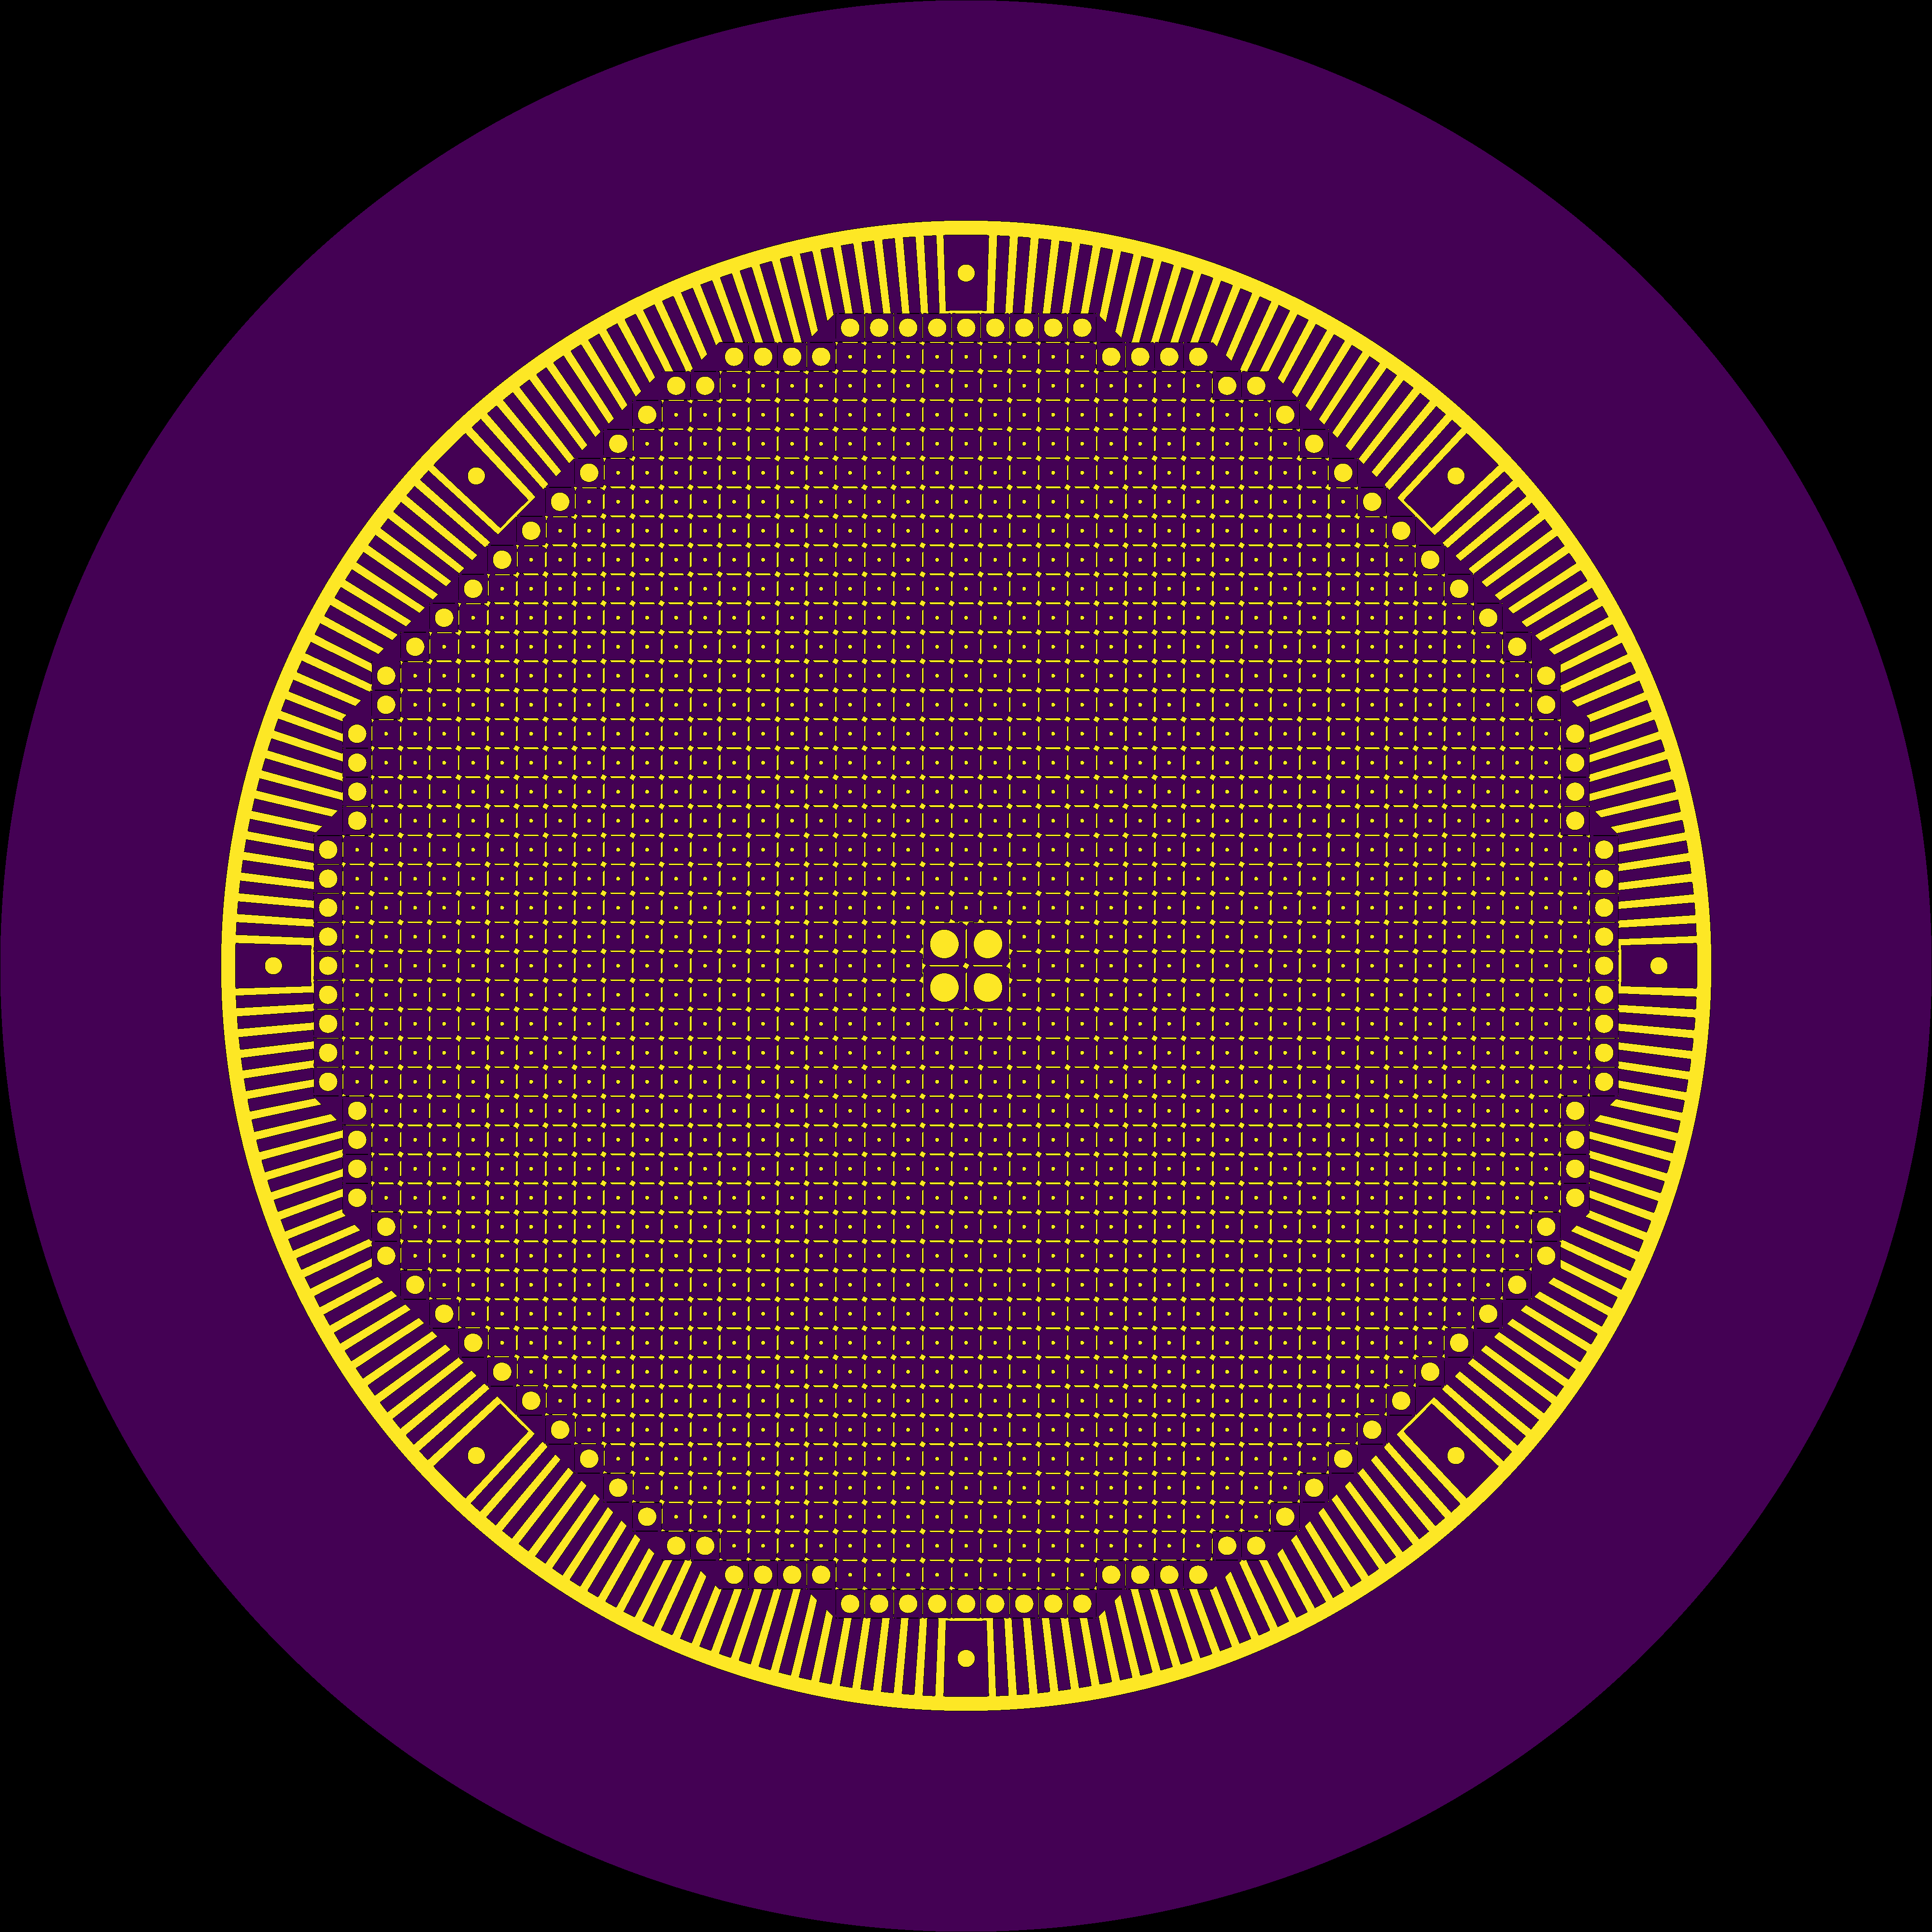
\includegraphics[width=0.45\textwidth]{./images/plan_msbr.png}
                        \includegraphics[width=0.45\textwidth]{./images/plan_msbr_results.png}
                        \caption{Above, full \gls{MSBR} core neutronics simulation in 
                        Serpent (Rykhlevskii et al. 2019
                        \cite{rykhlevskii_modeling_2019}). Left: geometry. 
                        Right: Monte Carlo Neutron Transport scattering and 
                        fission.}
                \end{figure}
        \end{center}
\end{frame}


\begin{frame}
        \frametitle{Moltres (coupling in MOOSE) (Lindsay et al. 2018 \cite{lindsay_introduction_2018})}
  \begin{figure}
   \vspace{-0.05in}
   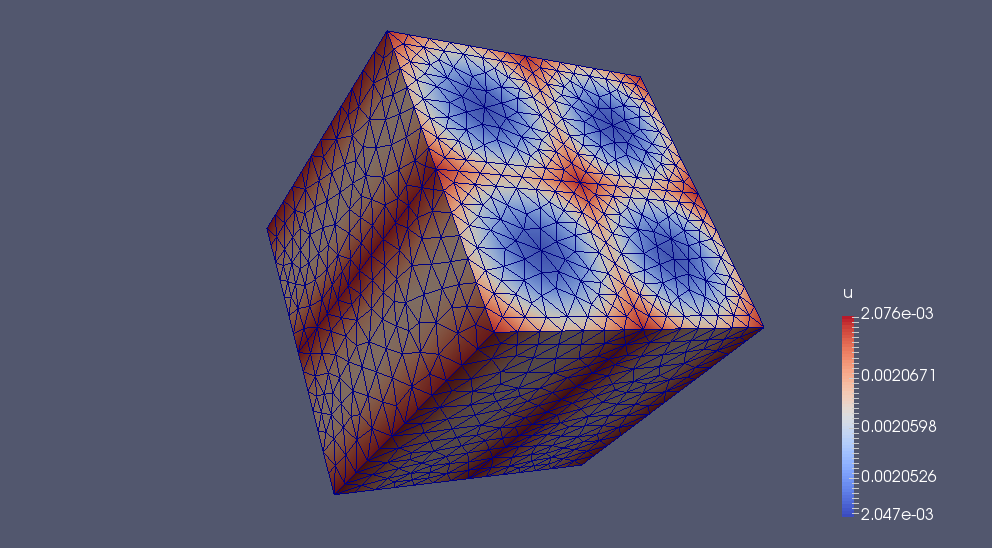
\includegraphics[height=0.75\textheight]{./images/lindsay_msre_moose.png}
    \end{figure}
\end{frame}



\begin{frame}
        \frametitle{Moltres Precursor Drift 
        (Lindsay et al. 2018 \cite{lindsay_introduction_2018})}
  \begin{figure}
   \vspace{-0.1in}
   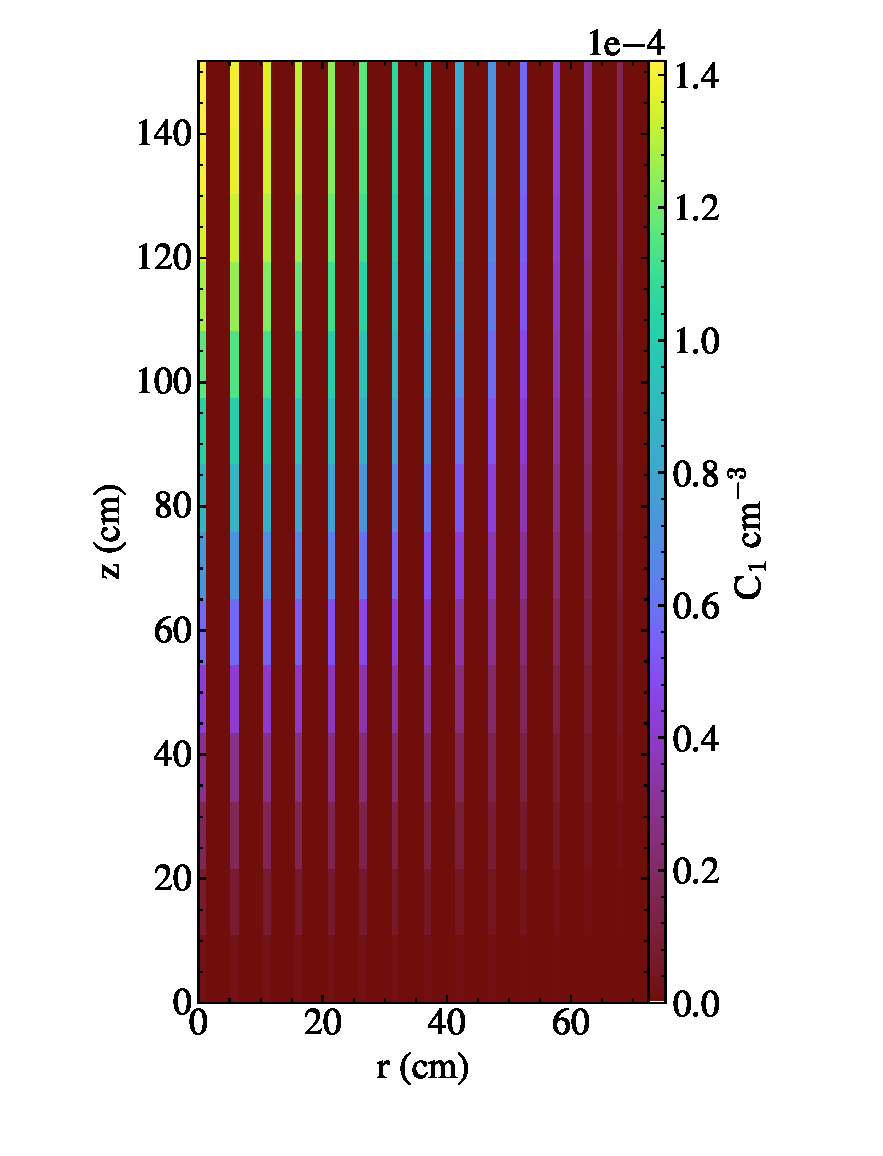
\includegraphics[width=0.28\textwidth]{./images/auto_diff_rho_pre1.eps}
   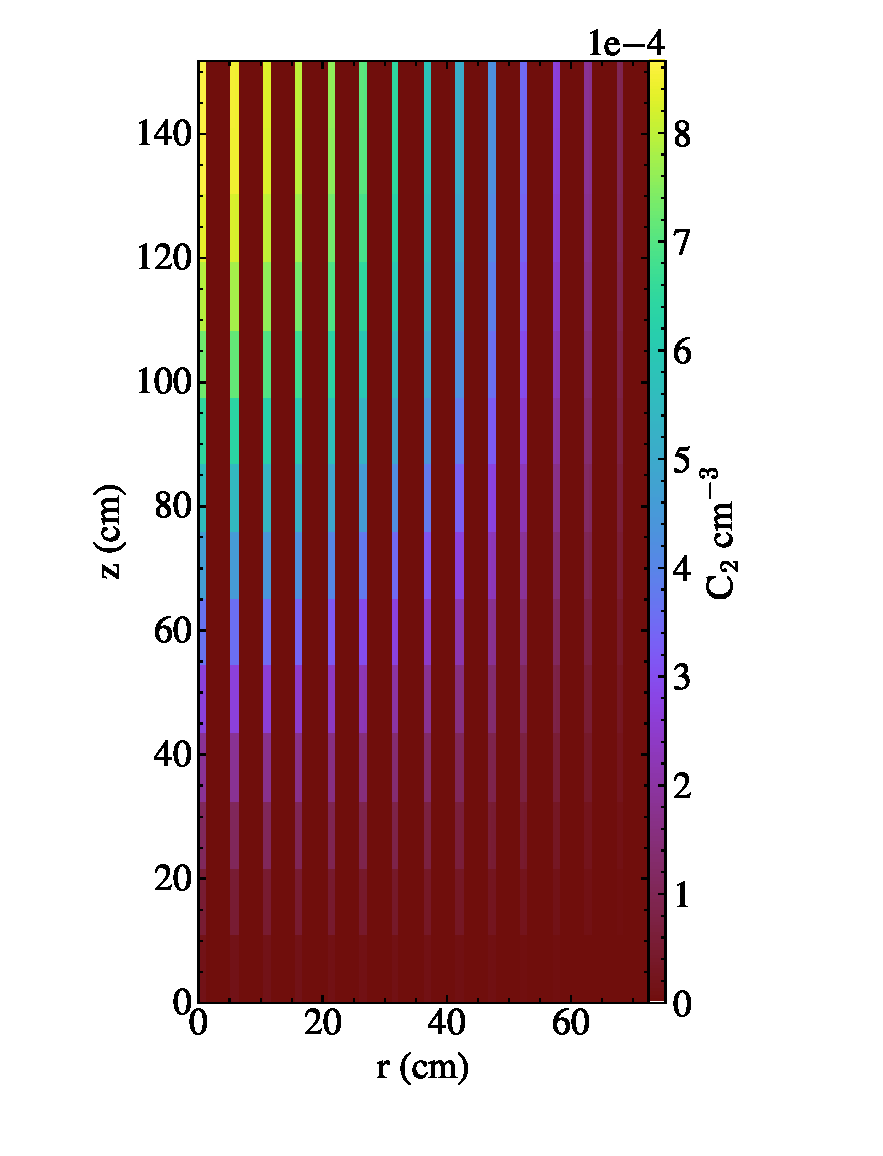
\includegraphics[width=0.28\textwidth]{./images/auto_diff_rho_pre2.eps}
   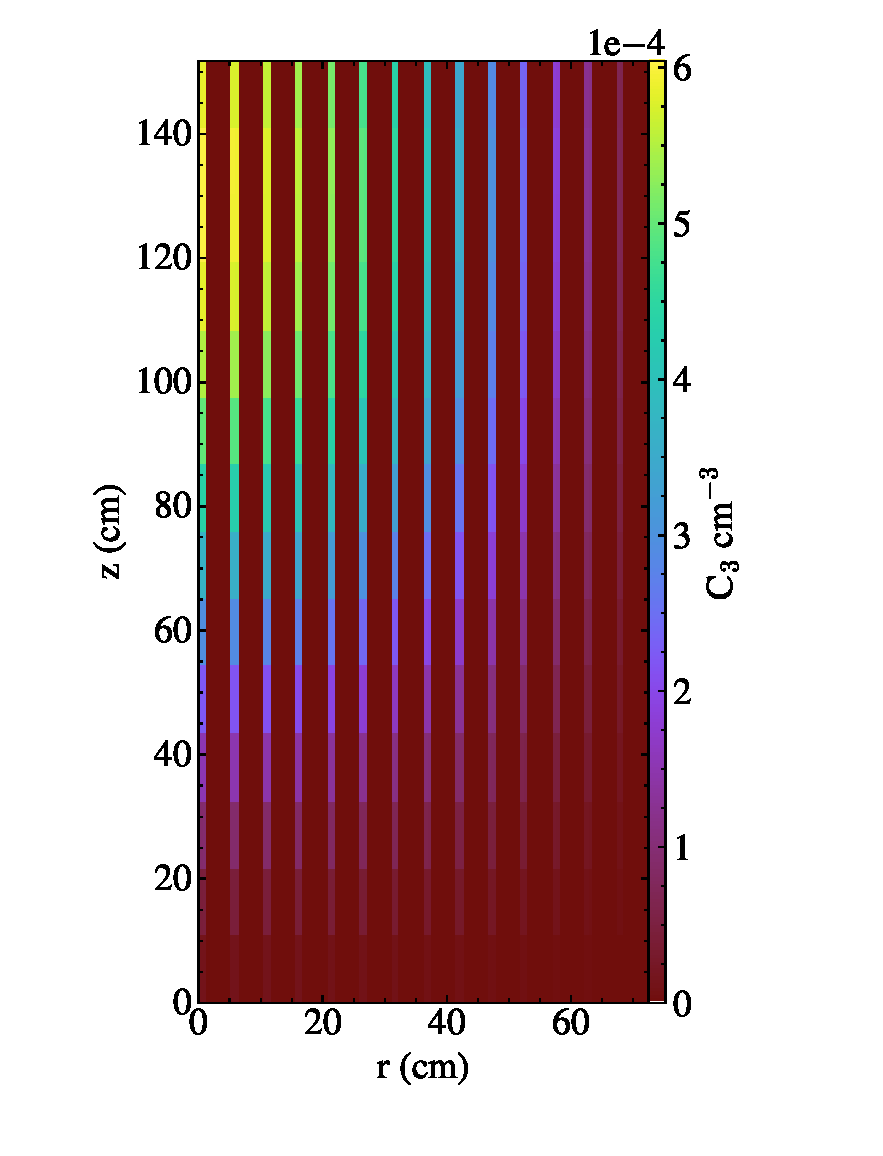
\includegraphics[width=0.28\textwidth]{./images/auto_diff_rho_pre3.eps}
   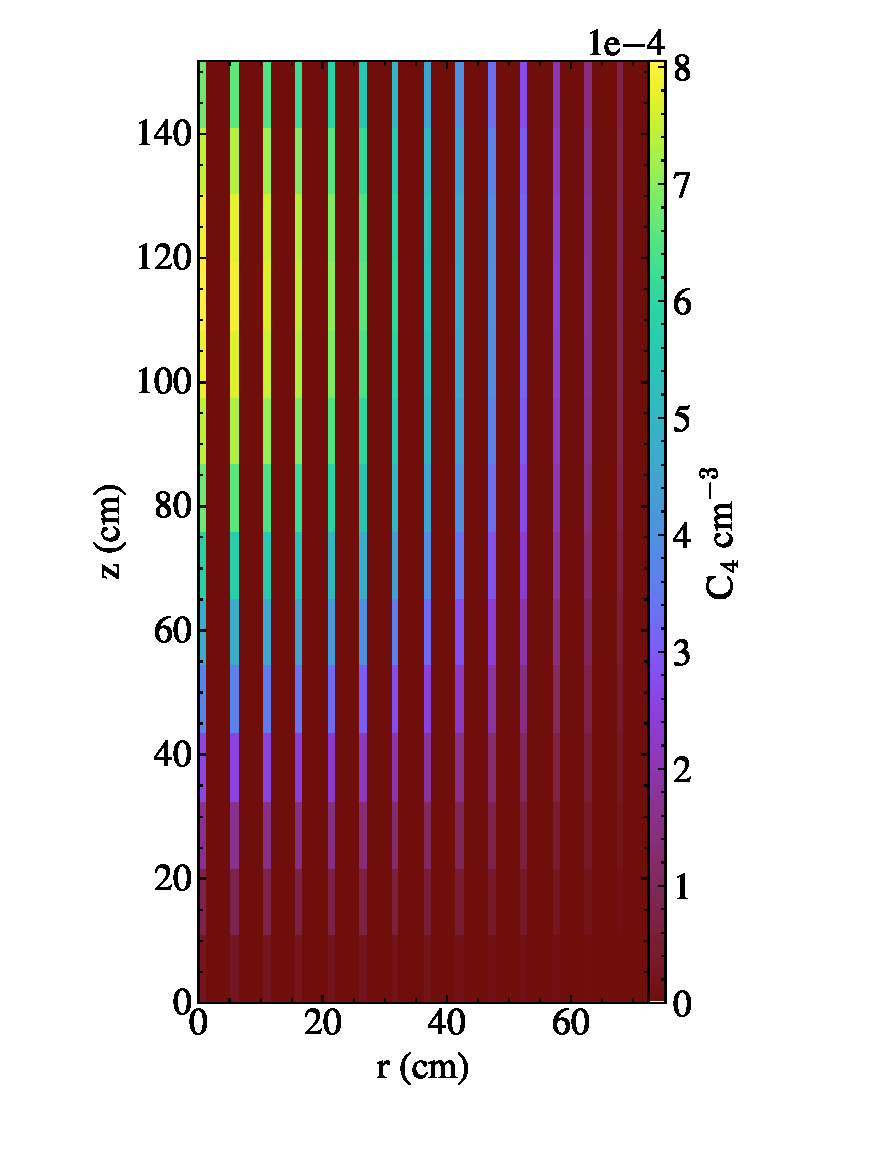
\includegraphics[width=0.28\textwidth]{./images/auto_diff_rho_pre4.eps}
   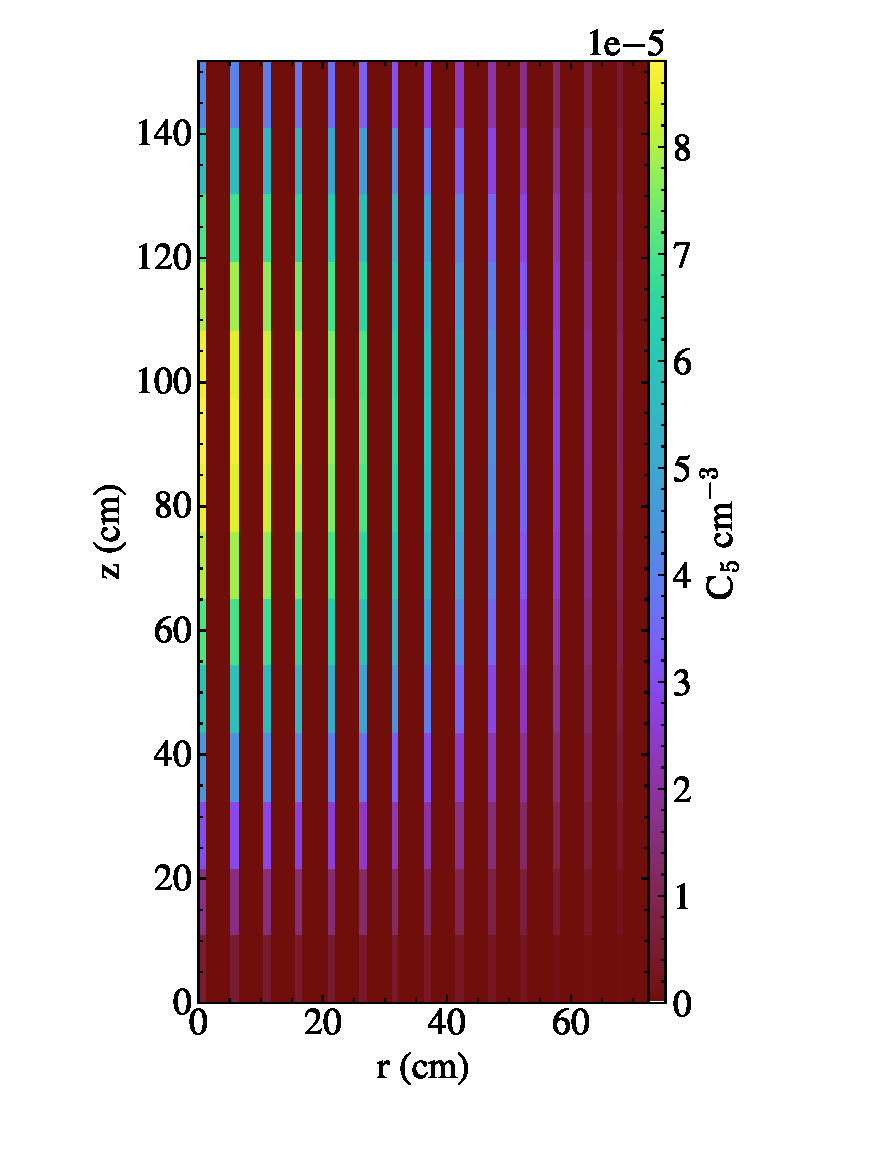
\includegraphics[width=0.28\textwidth]{./images/auto_diff_rho_pre5.eps}
   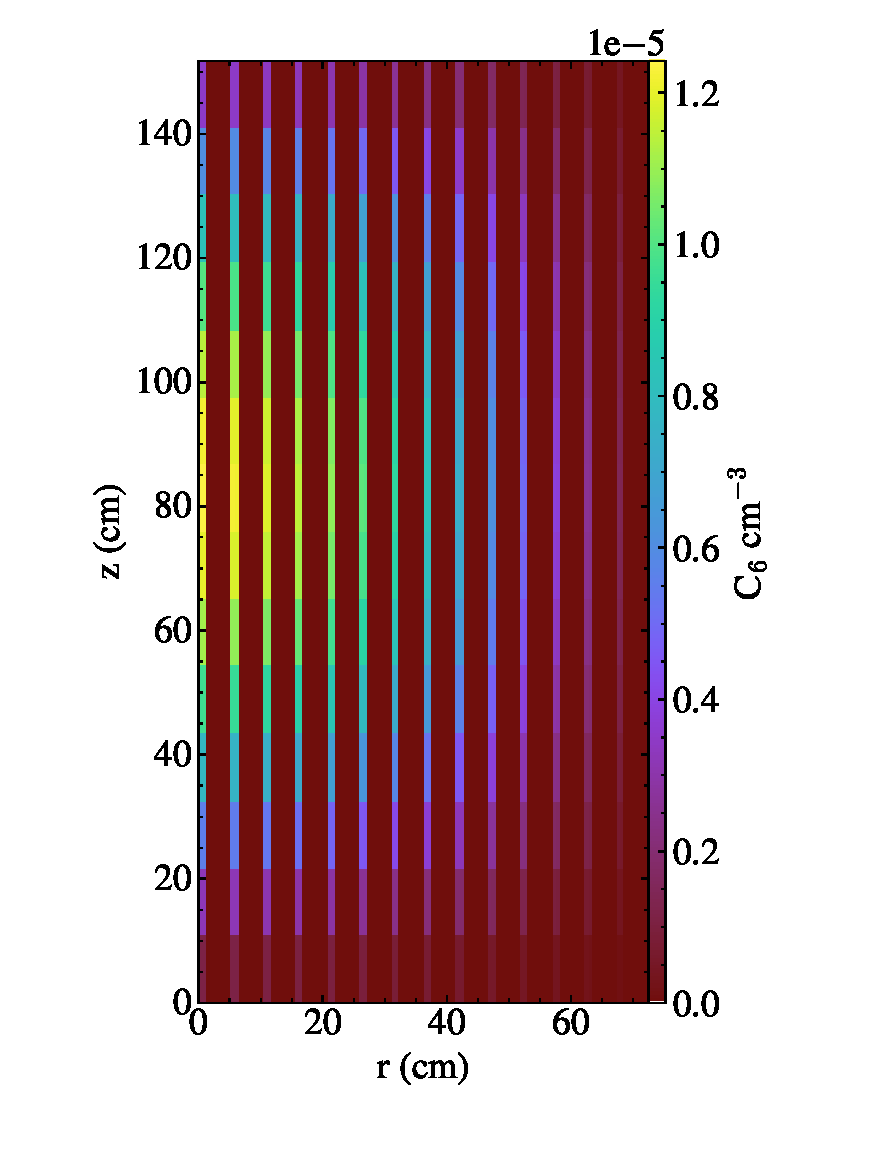
\includegraphics[width=0.28\textwidth]{./images/auto_diff_rho_pre6.eps}
    \end{figure}
\end{frame}



\begin{frame}
  \frametitle{Multiphysics simulation results (3D)}
  \begin{figure}[t]
   \vspace{-0.1in}
   \hspace*{-0.45in}
   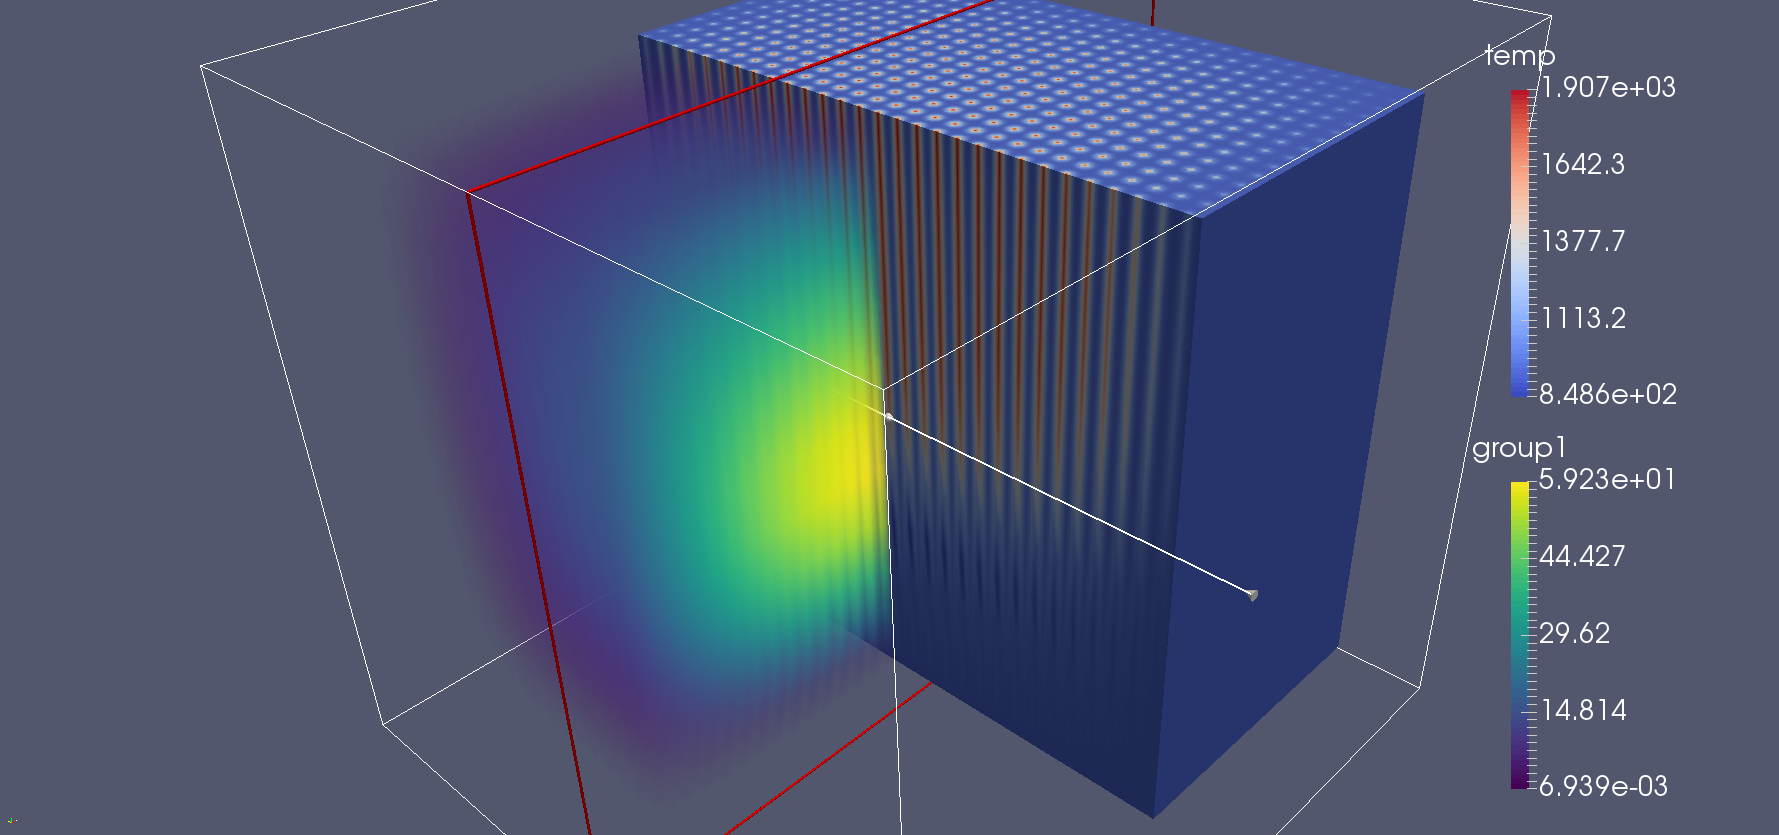
\includegraphics[height=0.75\textheight]{./images/moltres_3D.png}
   \caption{Cuboidal \gls{MSR} steady-state temperature and fast neutron flux 
          tests by Gavin Ridley.} 
    \end{figure}

\end{frame}

\begin{frame}
  \frametitle{Conclusions}
        \begin{block}{This study outcomes}
        \begin{itemize}
                \item New tool SaltProc was developed to simulate fuel depletion in the \gls{MSR} core with taking into account online reprocessing.
                \item SaltProc was tested for \gls{MSBR} conceptial design, equilibrium fuel salt composition was found and verified against recent \gls{ORNL} studies.
		\item Average $^{232}$Th refill rate throughout 20 years of operation is approximately 2.39 kg/day or 100 g/GWh$_e$.
		\vspace*{0.15in}
		\item New tool Moltres was developed for modeling coupled physics in fluid-fuelled, molten salt reactors.
		\item The 2D-axisymmetric and 3D multiphysics models are presented.
		\item Moltres demonstrated strong parallel scaling (up to 384 physical cores) on a typical model problem but further optimization required.
		\item Over 55'000 node-hours were consumed on Blue Waters to perform this research.
        \end{itemize}
        \end{block}
        
\end{frame}

\begin{frame}
  \frametitle{Future research}
         
              \begin{block}{Future research effort}
                 \begin{enumerate}
                \item Equilibrium state search for Transatomic \gls{MSR} (\textgreater 30'000 node-hours).
                \item Fuel cycle performance analysis for load-following regime \\ (\textgreater 40'000 node-hours).
                \item \gls{LWR} fuel transmutation in \gls{MSR} viability (\textgreater 30'000 node-hours).
		\vspace*{0.15in}
                \item Start exploring transients in Moltres, e.g. explore responses to reactivity insertion or gaseuos poisons removal (\textgreater 70'000 node-hours).
               \end{enumerate}
               \end{block}
\end{frame}

\begin{frame}
  \frametitle{Acknowledgement}
  \begin{itemize}
    \item This research is part of the Blue Waters sustained-petascale computing project, 
which is supported by the National Science Foundation (awards OCI-0725070 and 
ACI-1238993) and the state of Illinois.
    \item Andrei Rykhlevskii is supported by the Department of Nuclear, Plasma, and Radiological Engineering.
    \item Kathryn Huff is additionally supported by the NRC Faculty Development Program, the NNSA (awards 
    DE-NA0002576 and DE-NA0002534), and the International Institute for Carbon Neutral Energy Research (WPI-I2CNER).
    \item The authors would like to thank  members of Advanced Reactors and Fuel Cycles
research group (ARFC) at the University of Illinois - Urbana Champaign who 
provided valuable code reviews and proofreading.
    \item Alex Lindsay (Idaho National Laboratory), Gavin Ridley (University of Tennessee-Knoxville).
  \end{itemize}
    \begin{figure}[t]
   \hspace*{-0.4in}
   
\includegraphics[height=0.35\textheight]{./images/acks.png}
    \end{figure}
\end{frame}

%%--------------------------------%%
%%--------------------------------%%
\begin{frame}[allowframebreaks]
  \frametitle{References}
  \bibliographystyle{plain}
  {\footnotesize \bibliography{2018-huff-mumbai} }

\end{frame}

%%---BACKUP SLIDES----------------%%

\begin{frame}
  \frametitle{Processing options for \gls{MSR} fuels}
               \begin{figure}[t]
                \vspace*{-0.1in}
			\hspace{-0.3in}
                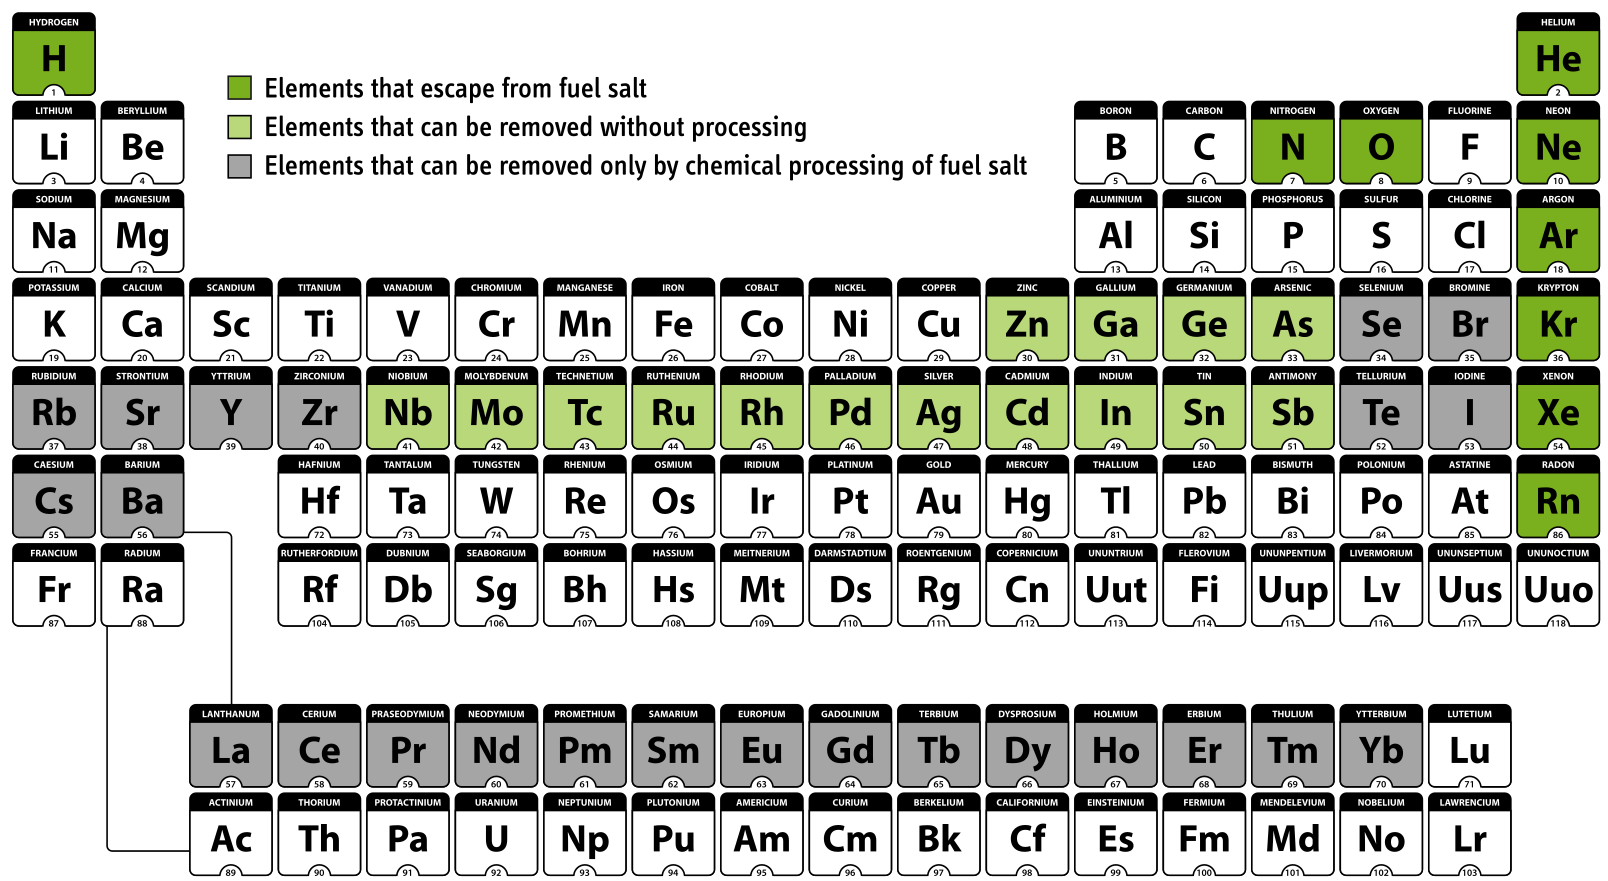
\includegraphics[height=0.6\textwidth]{./images/periodic_map.png}
               \end{figure}
              
\end{frame}

\begin{frame}
  \frametitle{BUBBLE GENERATOR AND GAS SEPARATOR for \gls{MSBR}}
               \begin{figure}[t]
                \vspace*{-0.1in}
                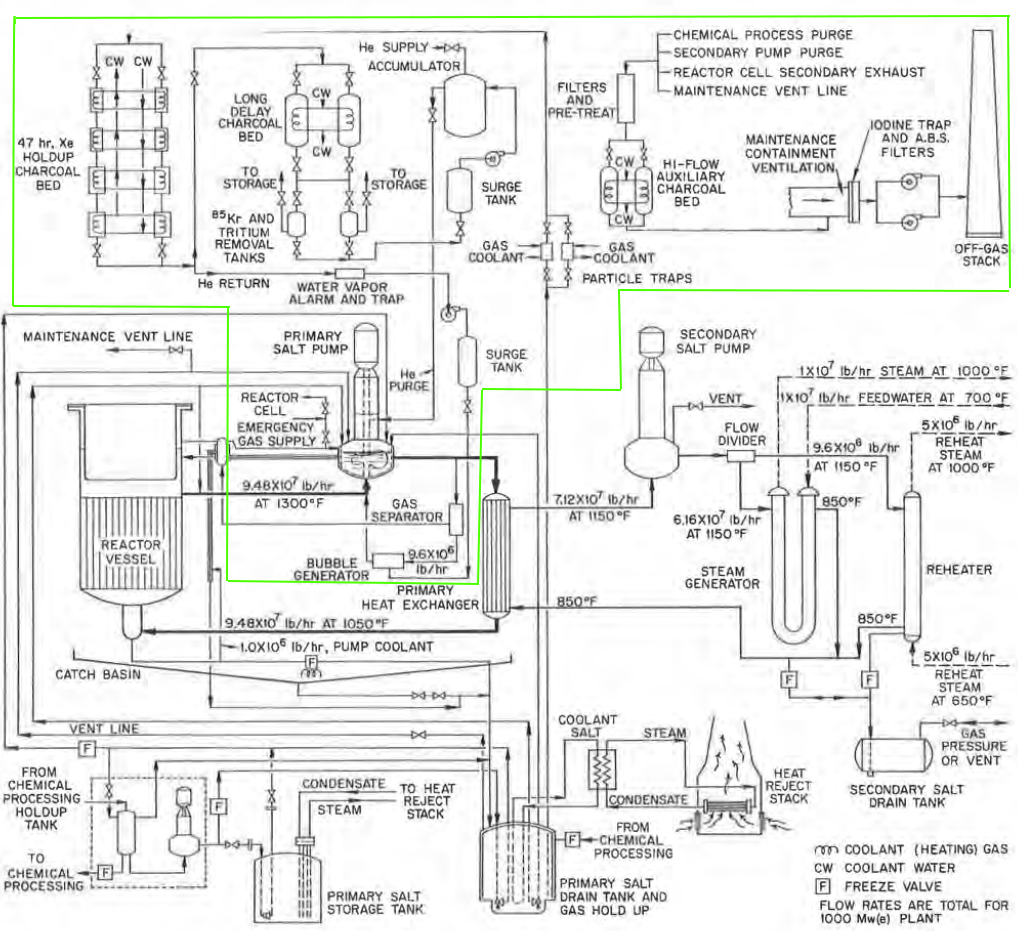
\includegraphics[height=0.7\textwidth]{./images/gas_separation.png}
               \end{figure}
              
\end{frame}

\begin{frame}
  \frametitle{Chemical processing facility for \gls{MSBR}}
               \begin{figure}[t]
                \vspace*{-0.1in}
                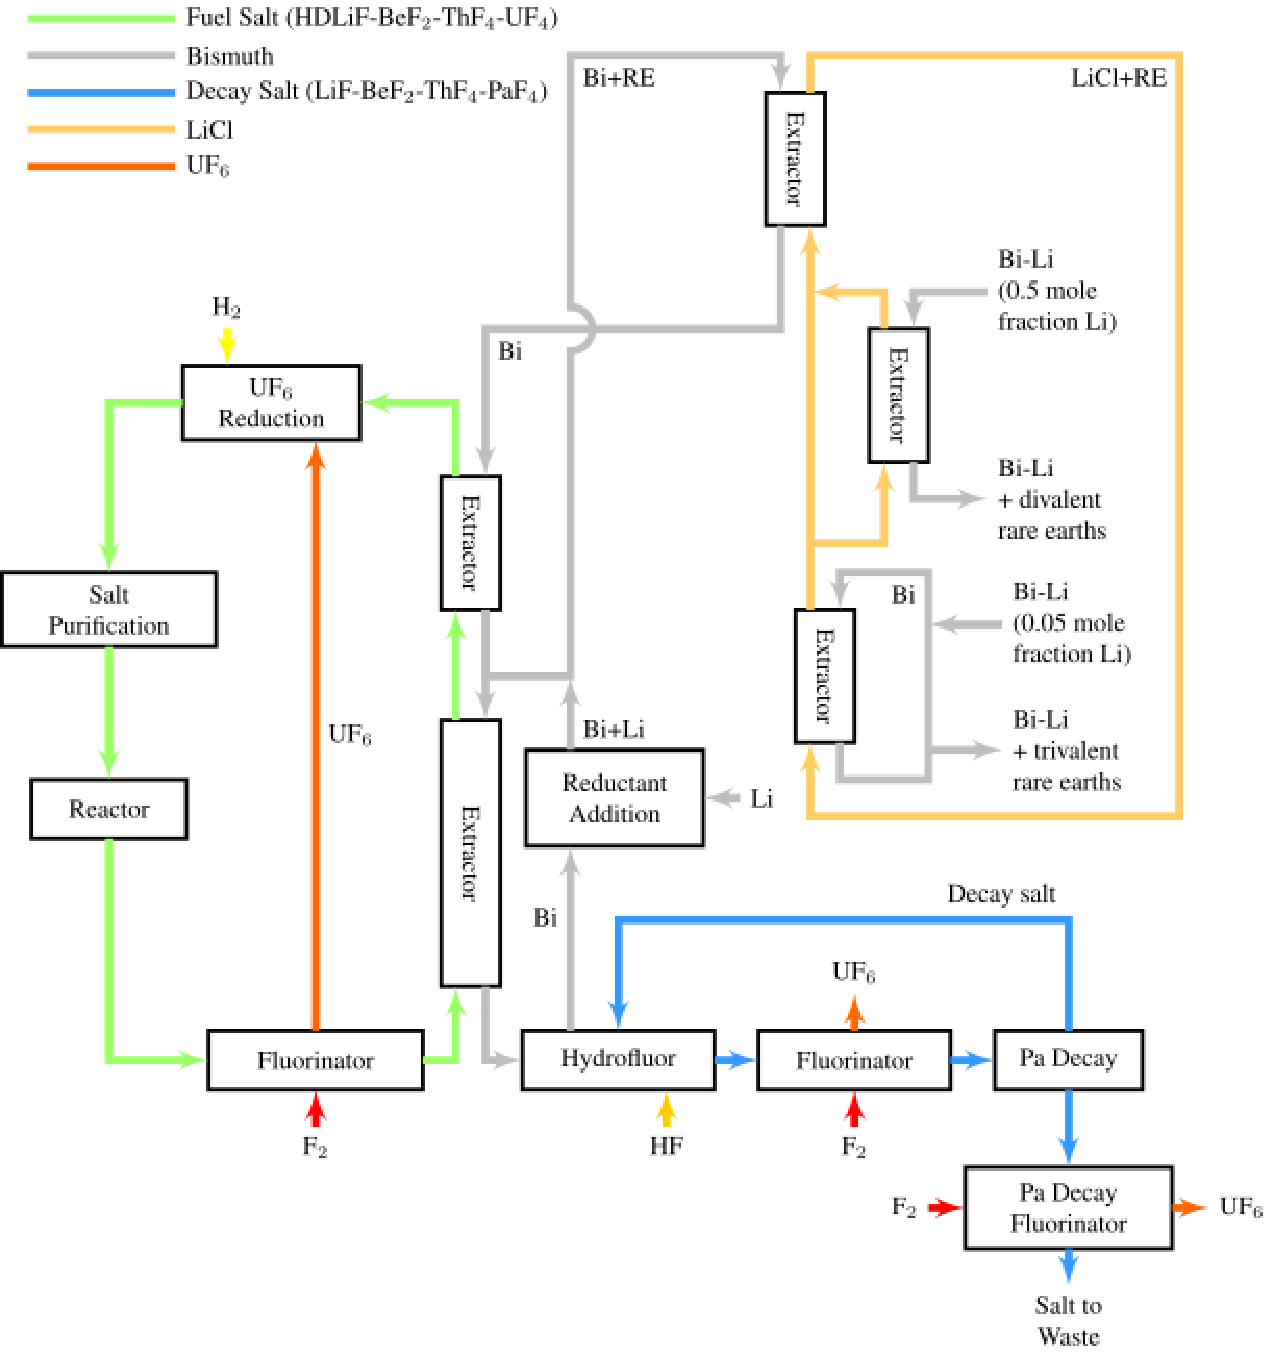
\includegraphics[height=0.65\textwidth]{./images/flowsheet.pdf}
               \end{figure}
              
\end{frame}

\begin{frame}
  \frametitle{Multiplication factor dynamics during Rb, Sr, Cs, Ba removal (3435days)}
               \begin{figure}[t]
                \vspace*{-0.1in}
                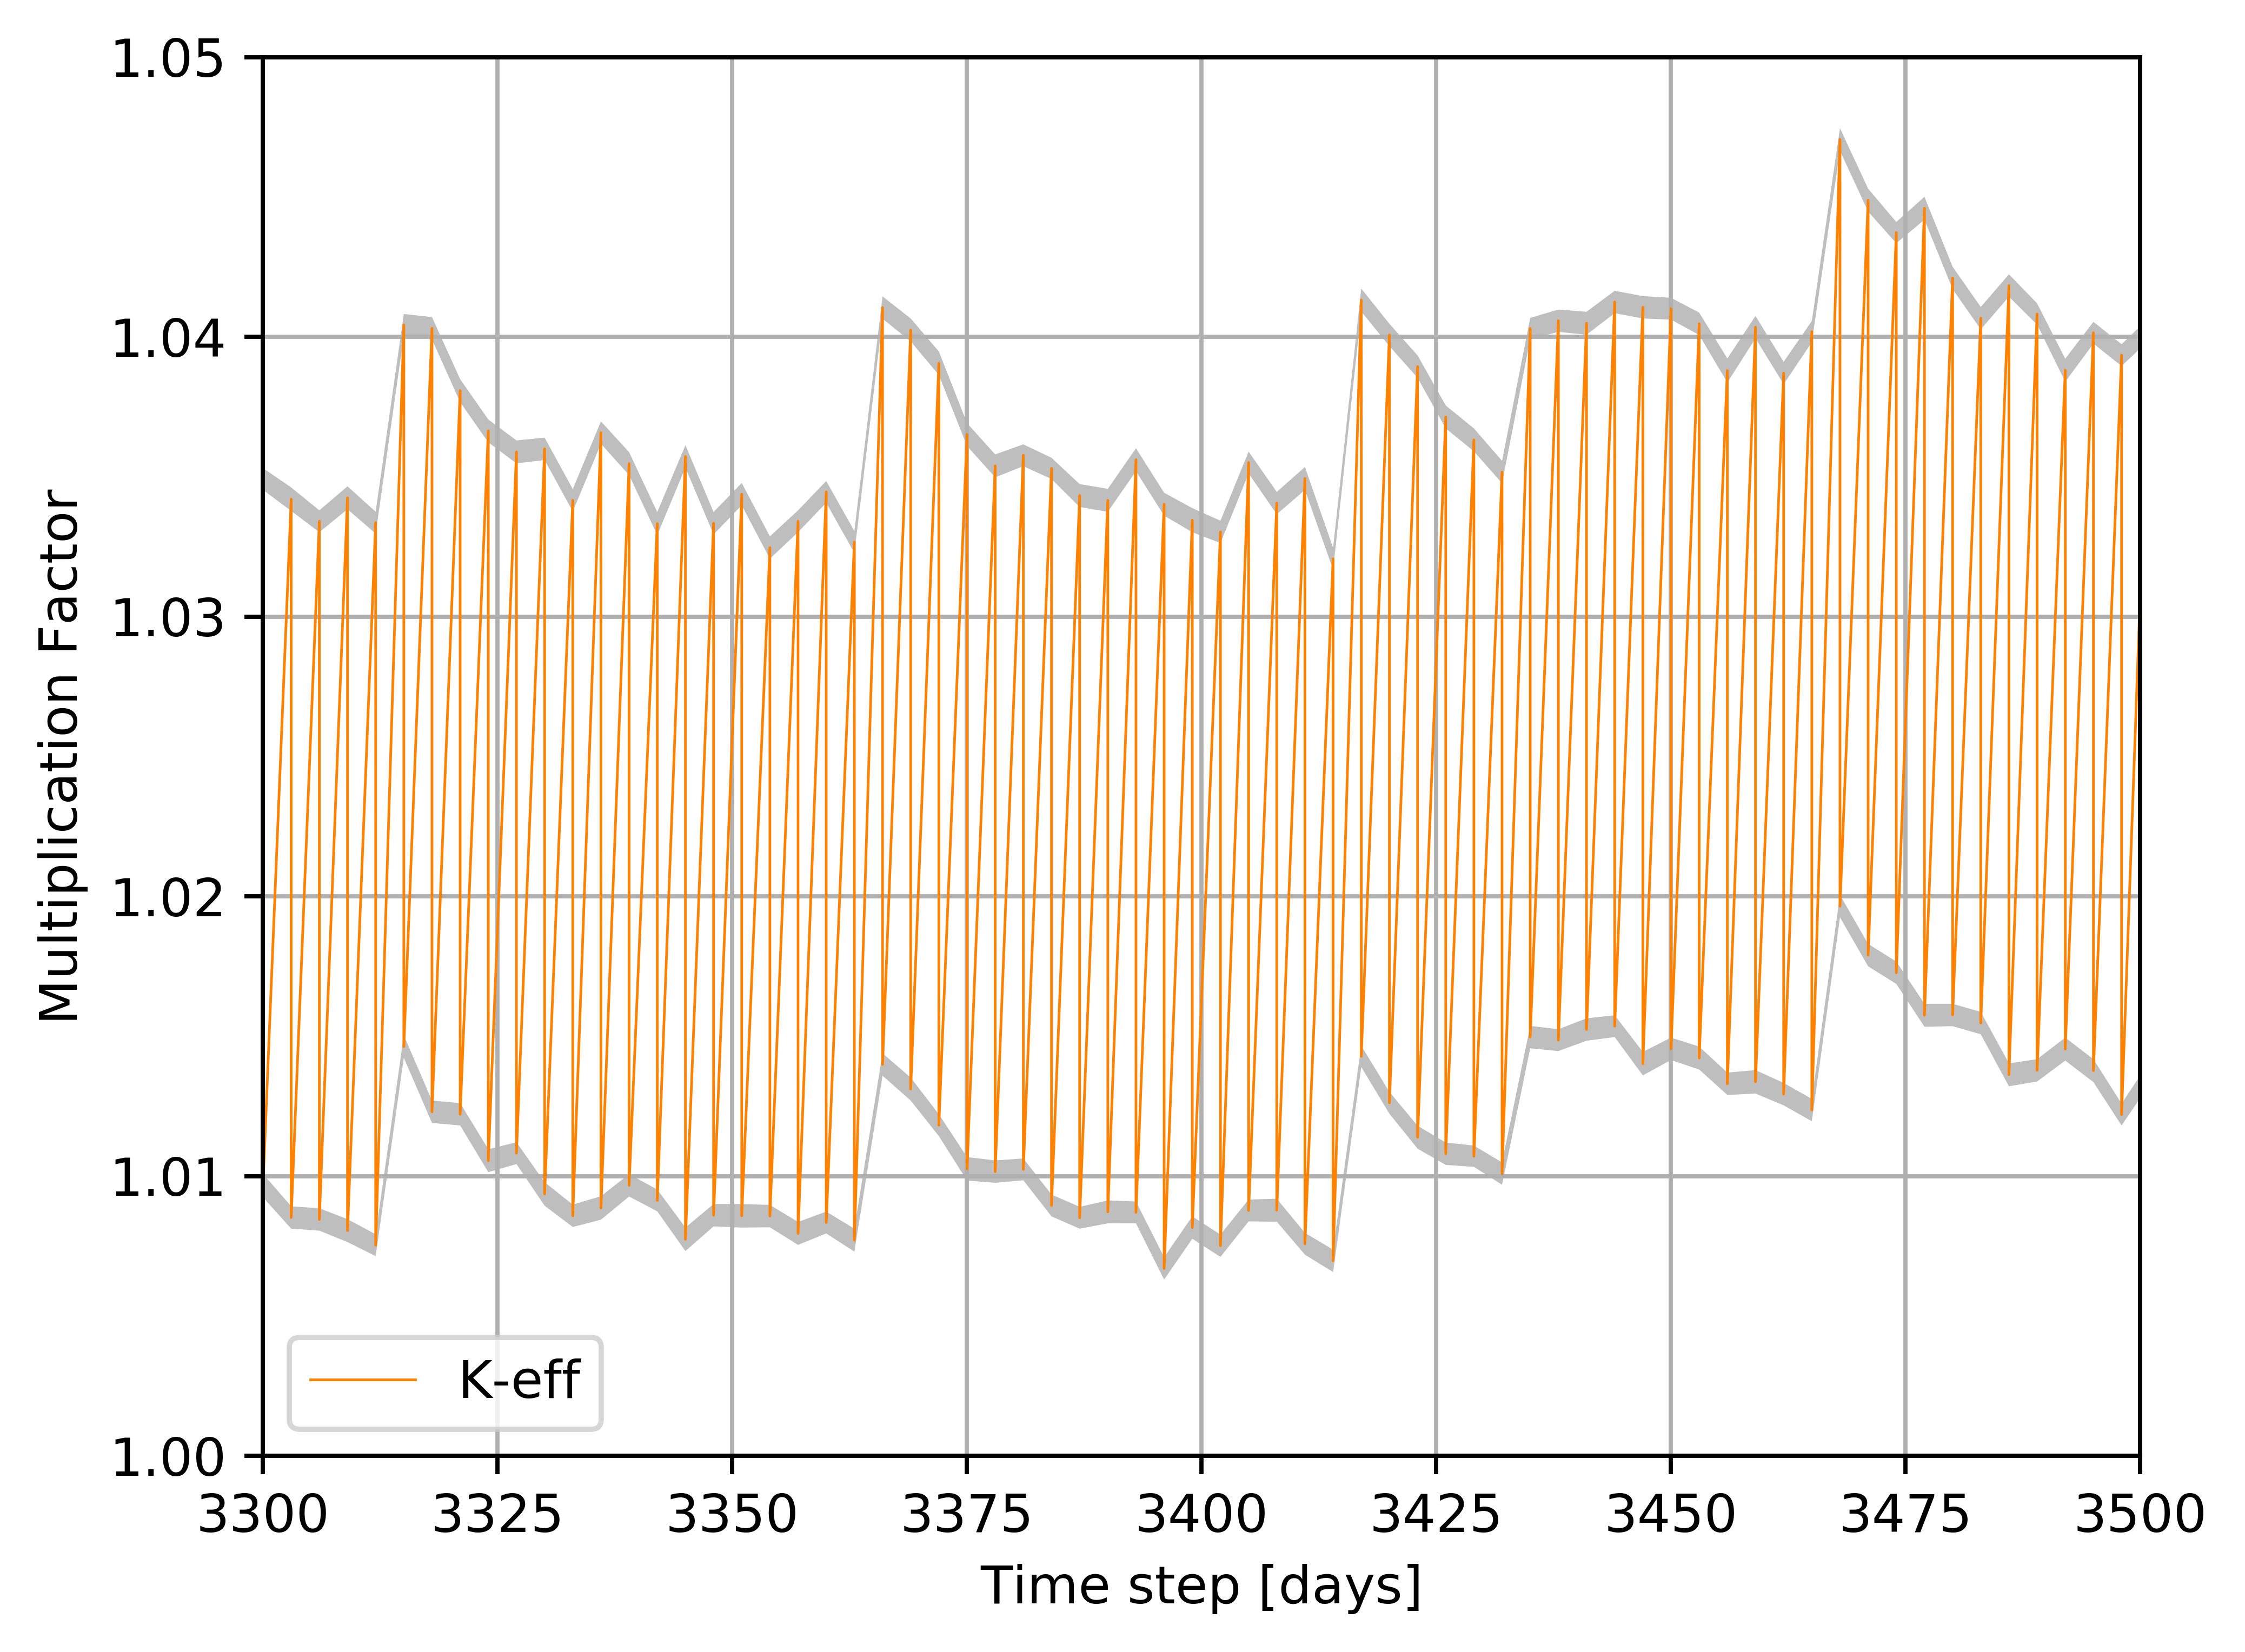
\includegraphics[height=0.7\textwidth]{./images/keff_3435st.png}
               \end{figure}
              
\end{frame}


\begin{frame}
  \frametitle{\gls{MSBR} neutron energy spectrum for different regions}
               \begin{figure}[t]
                \vspace*{-0.1in}
                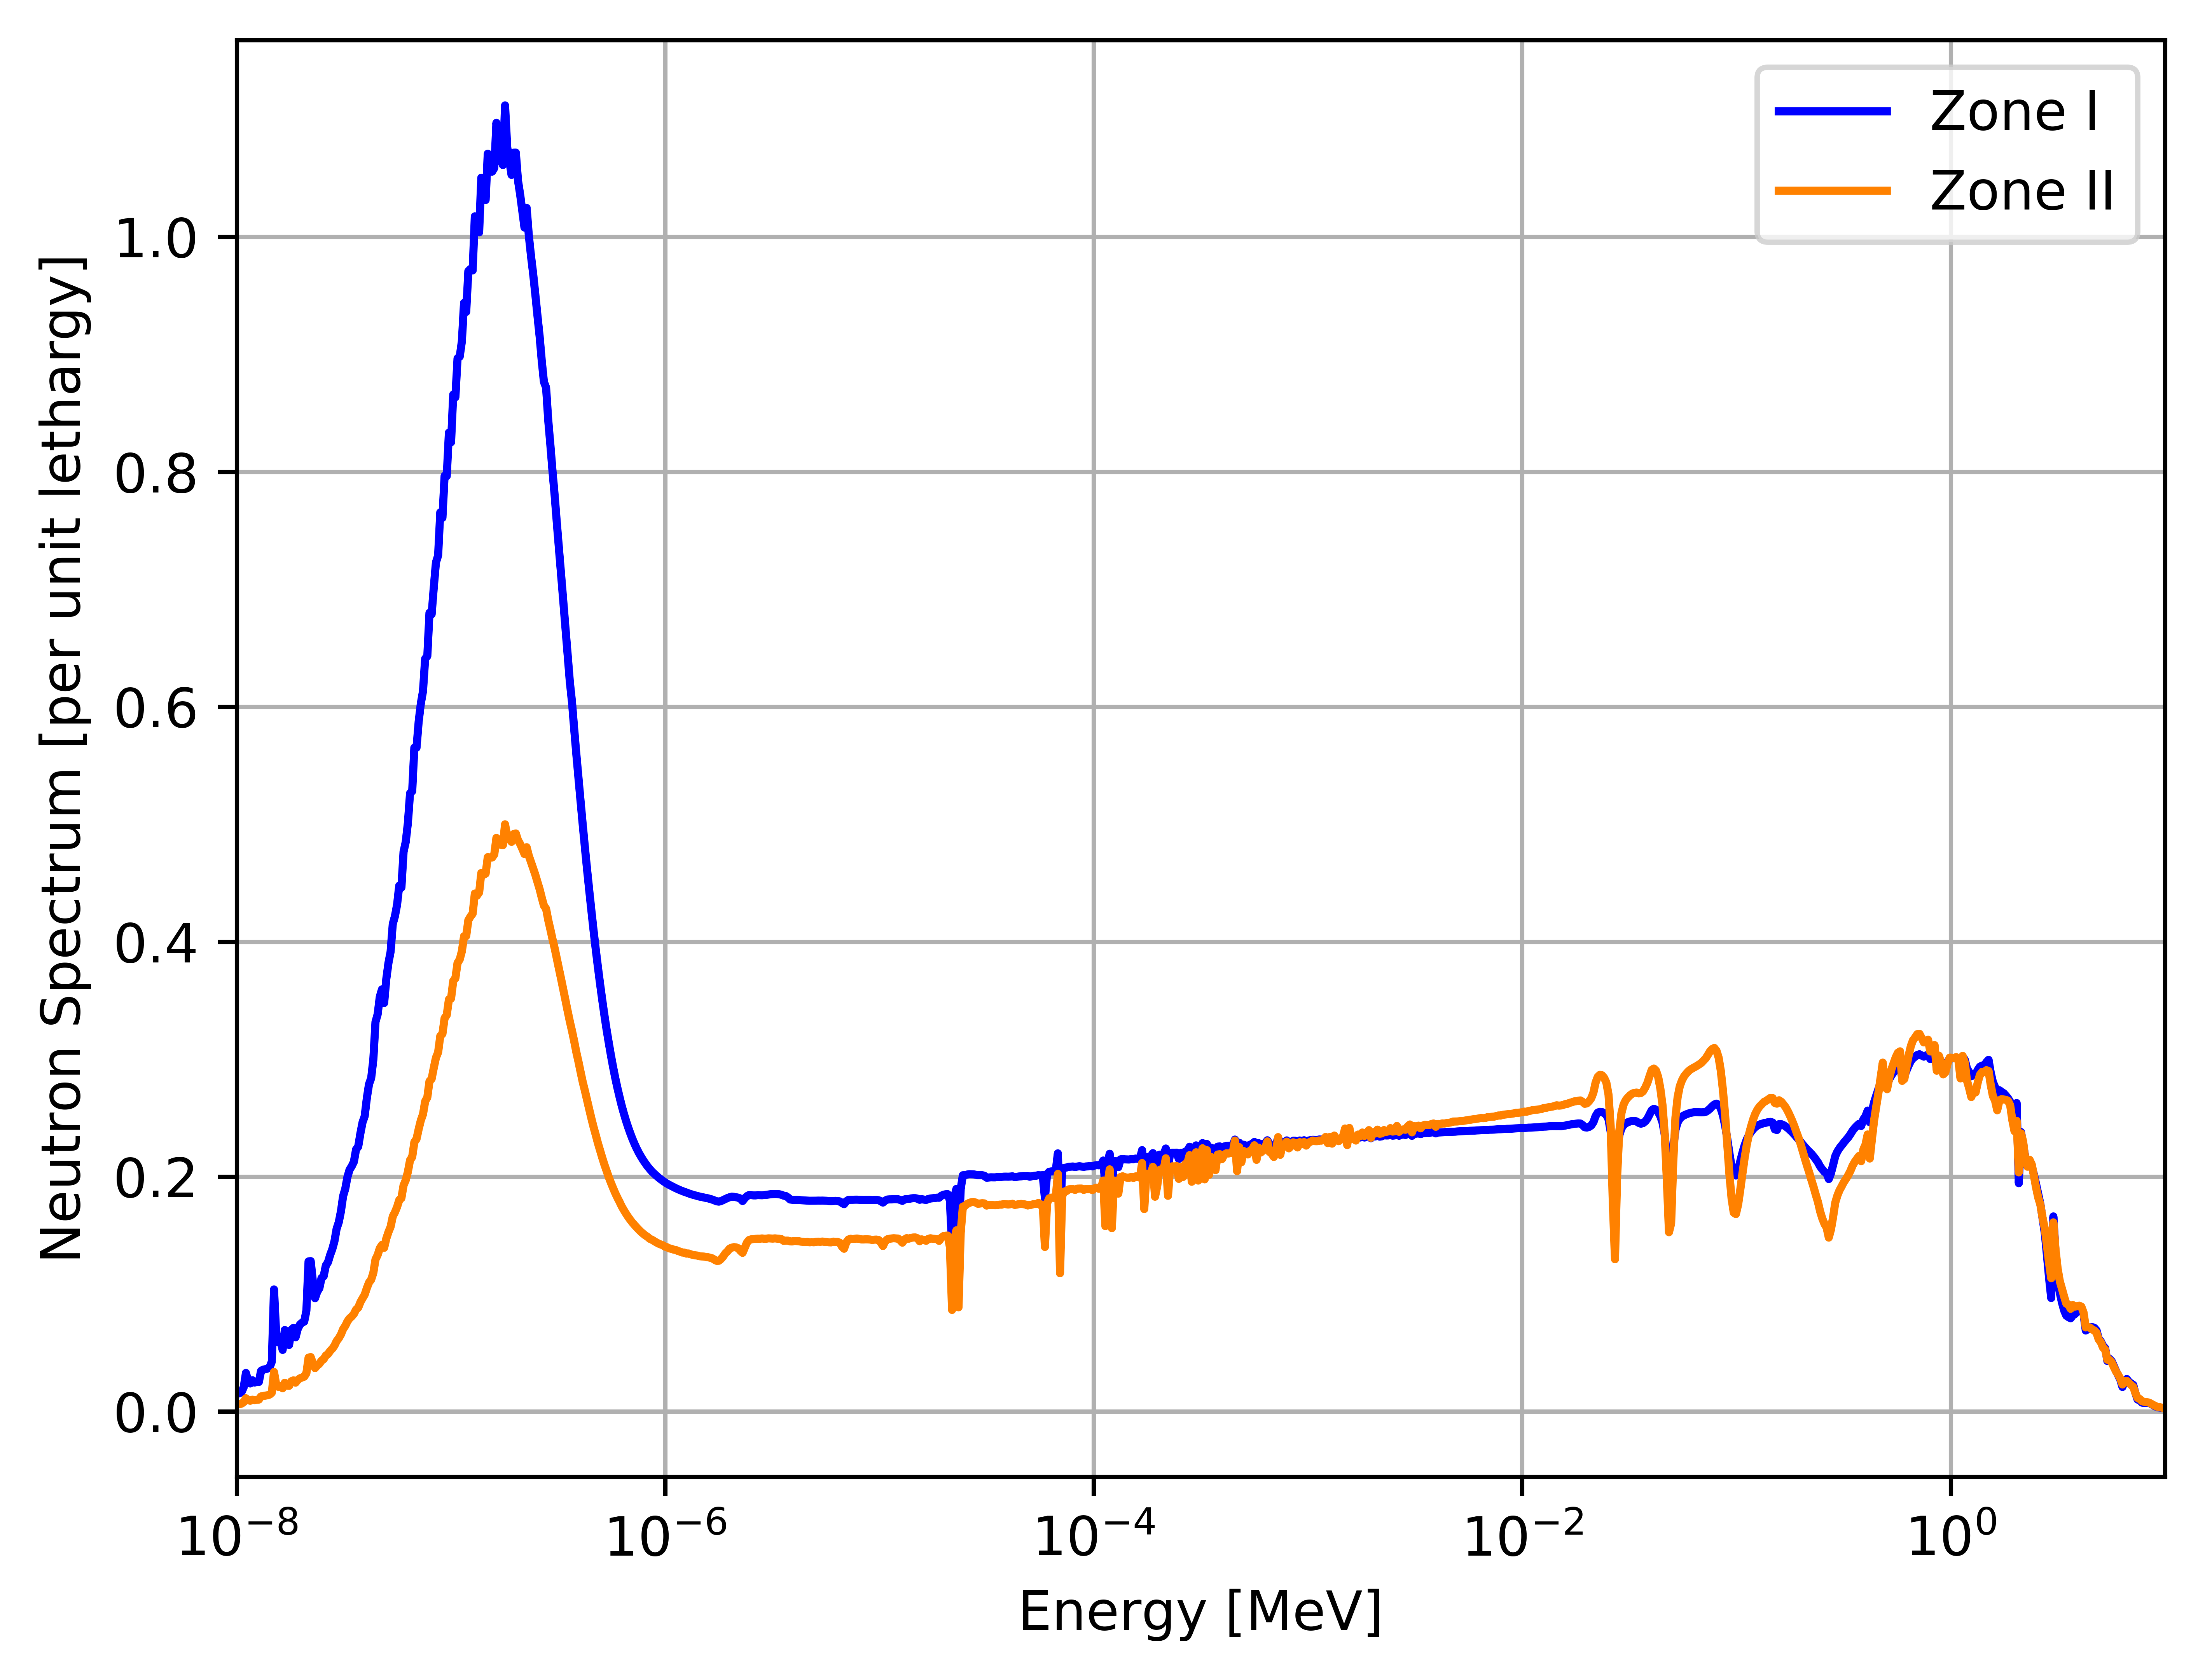
\includegraphics[height=0.35\textwidth]{./images/spectrum_zones_init.png}
               \end{figure}
               \begin{figure}[t]
                \vspace*{-0.1in}
                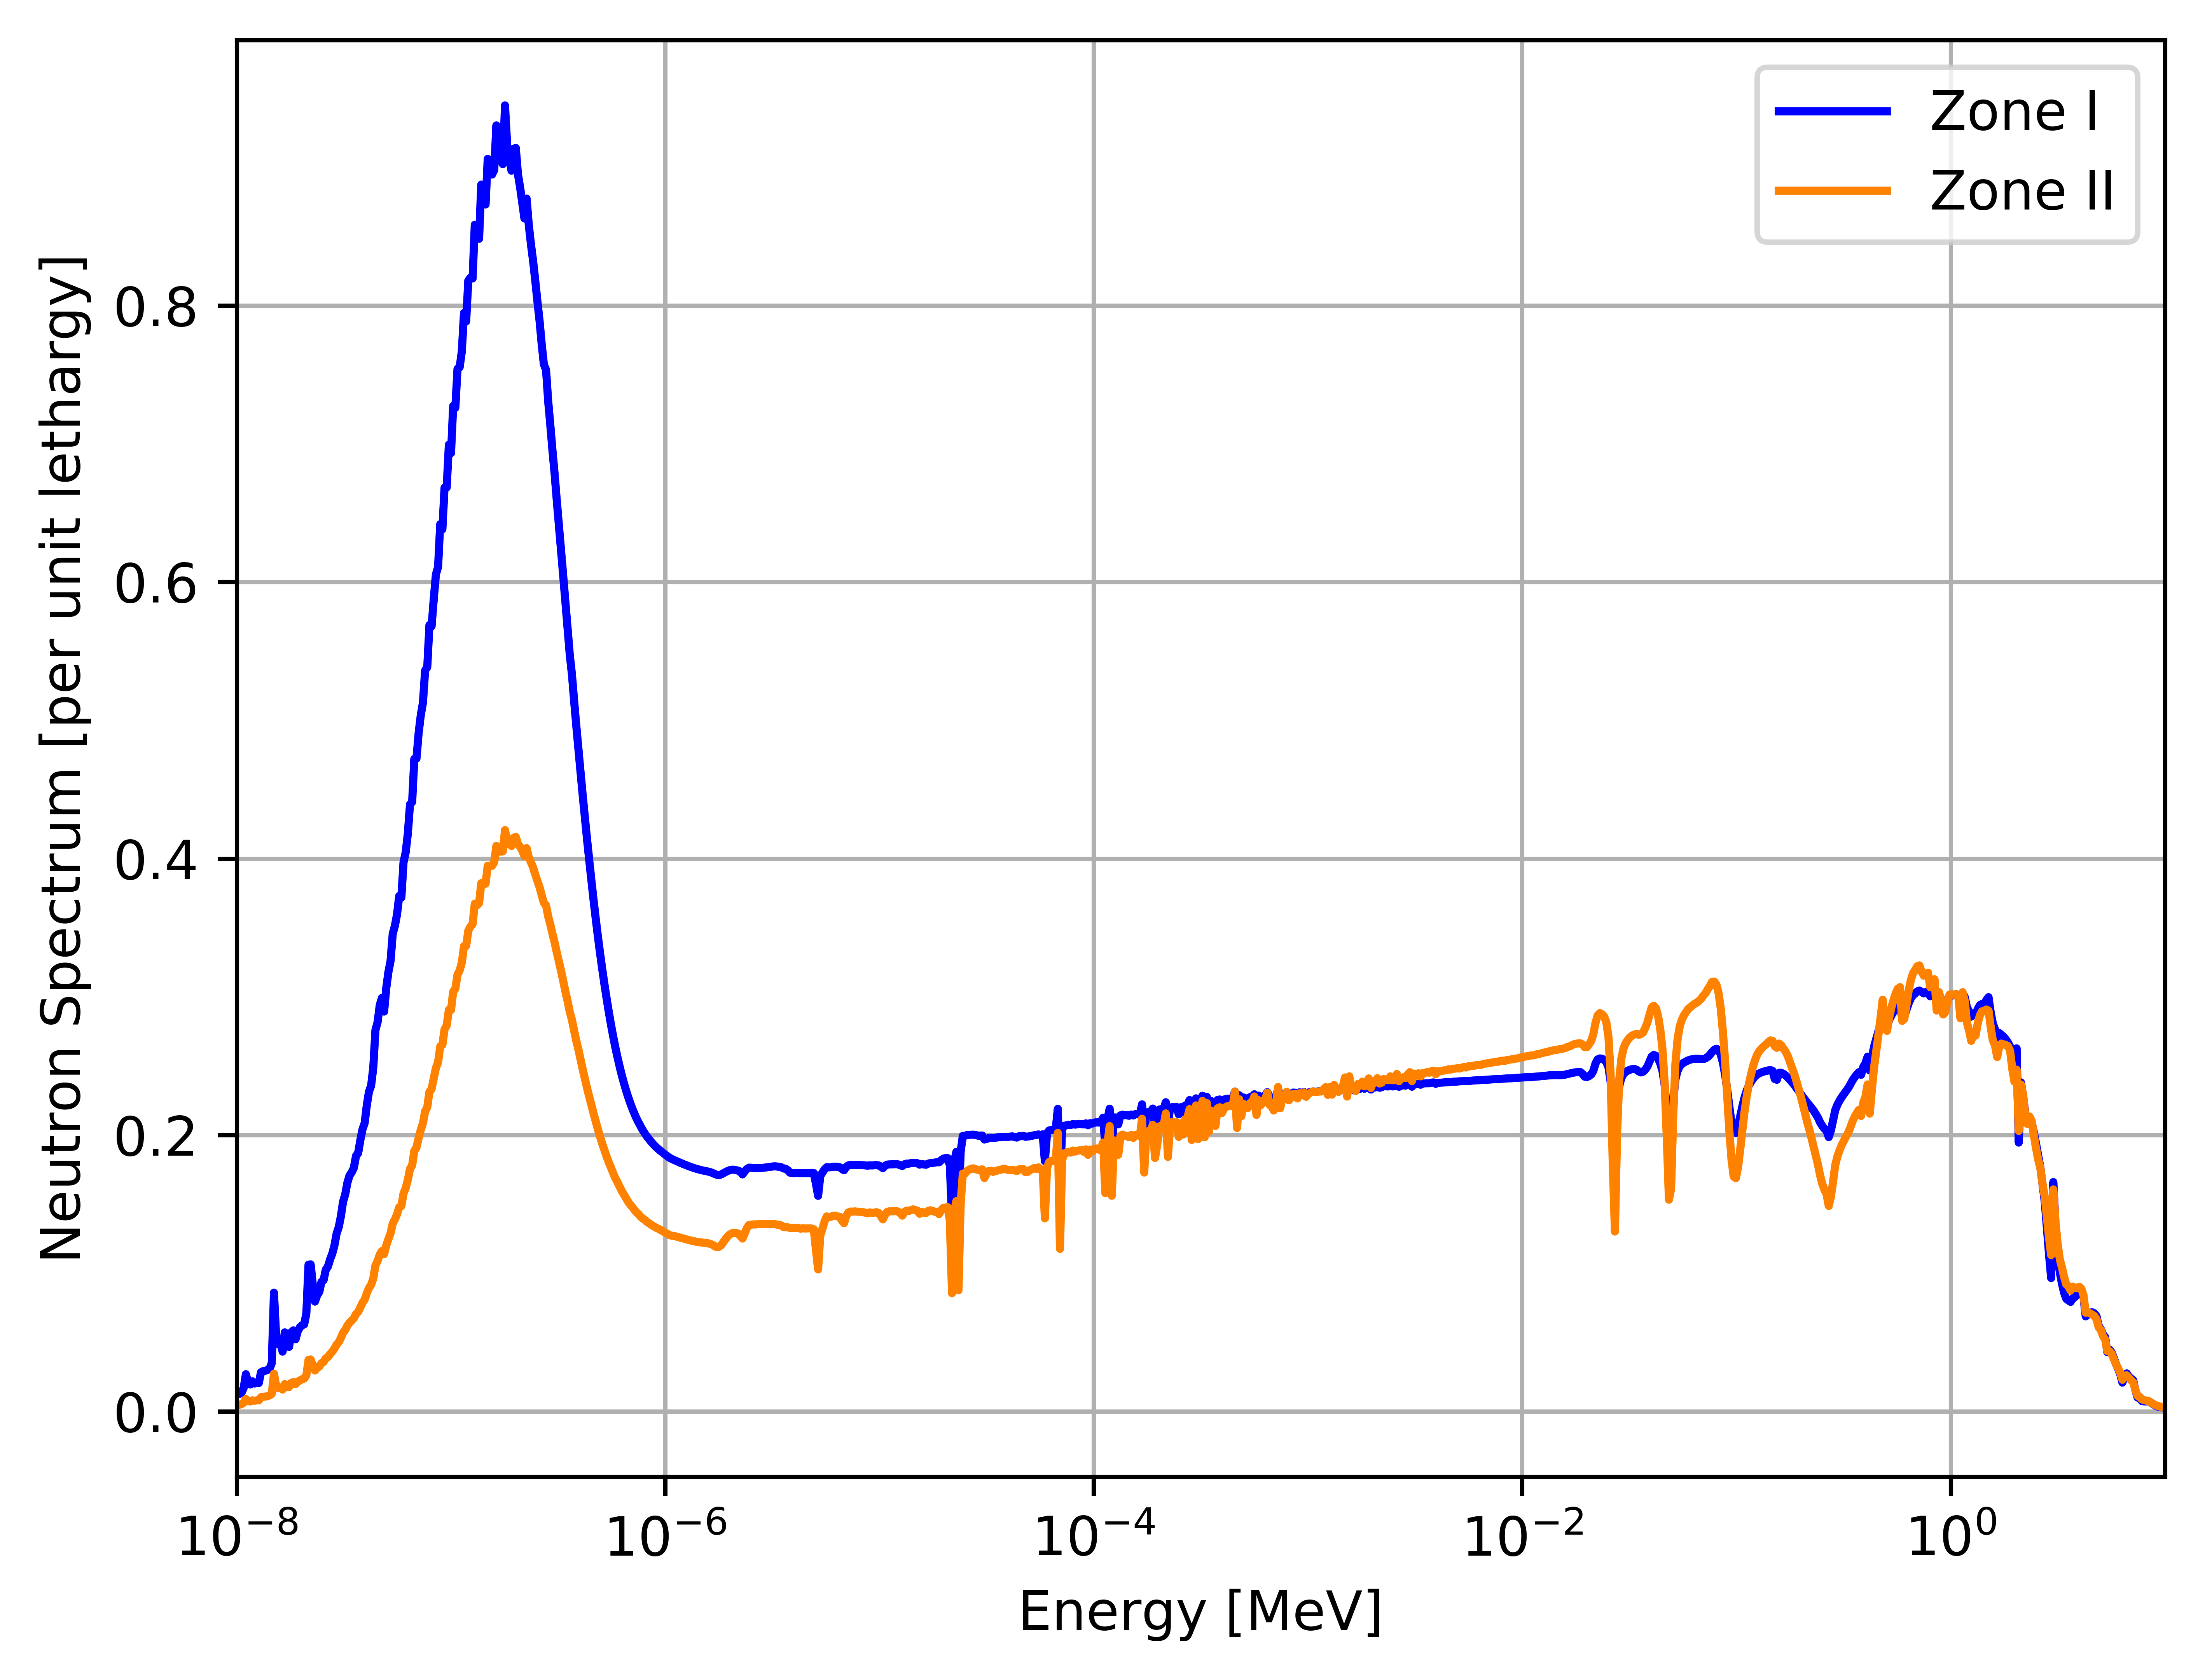
\includegraphics[height=0.35\textwidth]{./images/spectrum_zones_eq.png}
               \end{figure}
              
\end{frame}

\begin{frame}
  \frametitle{Fissile isotopes in the \gls{MSBR} core}
  \begin{columns}
    \column[t]{6cm}
               \begin{figure}[t]
                \vspace*{-0.1in}
                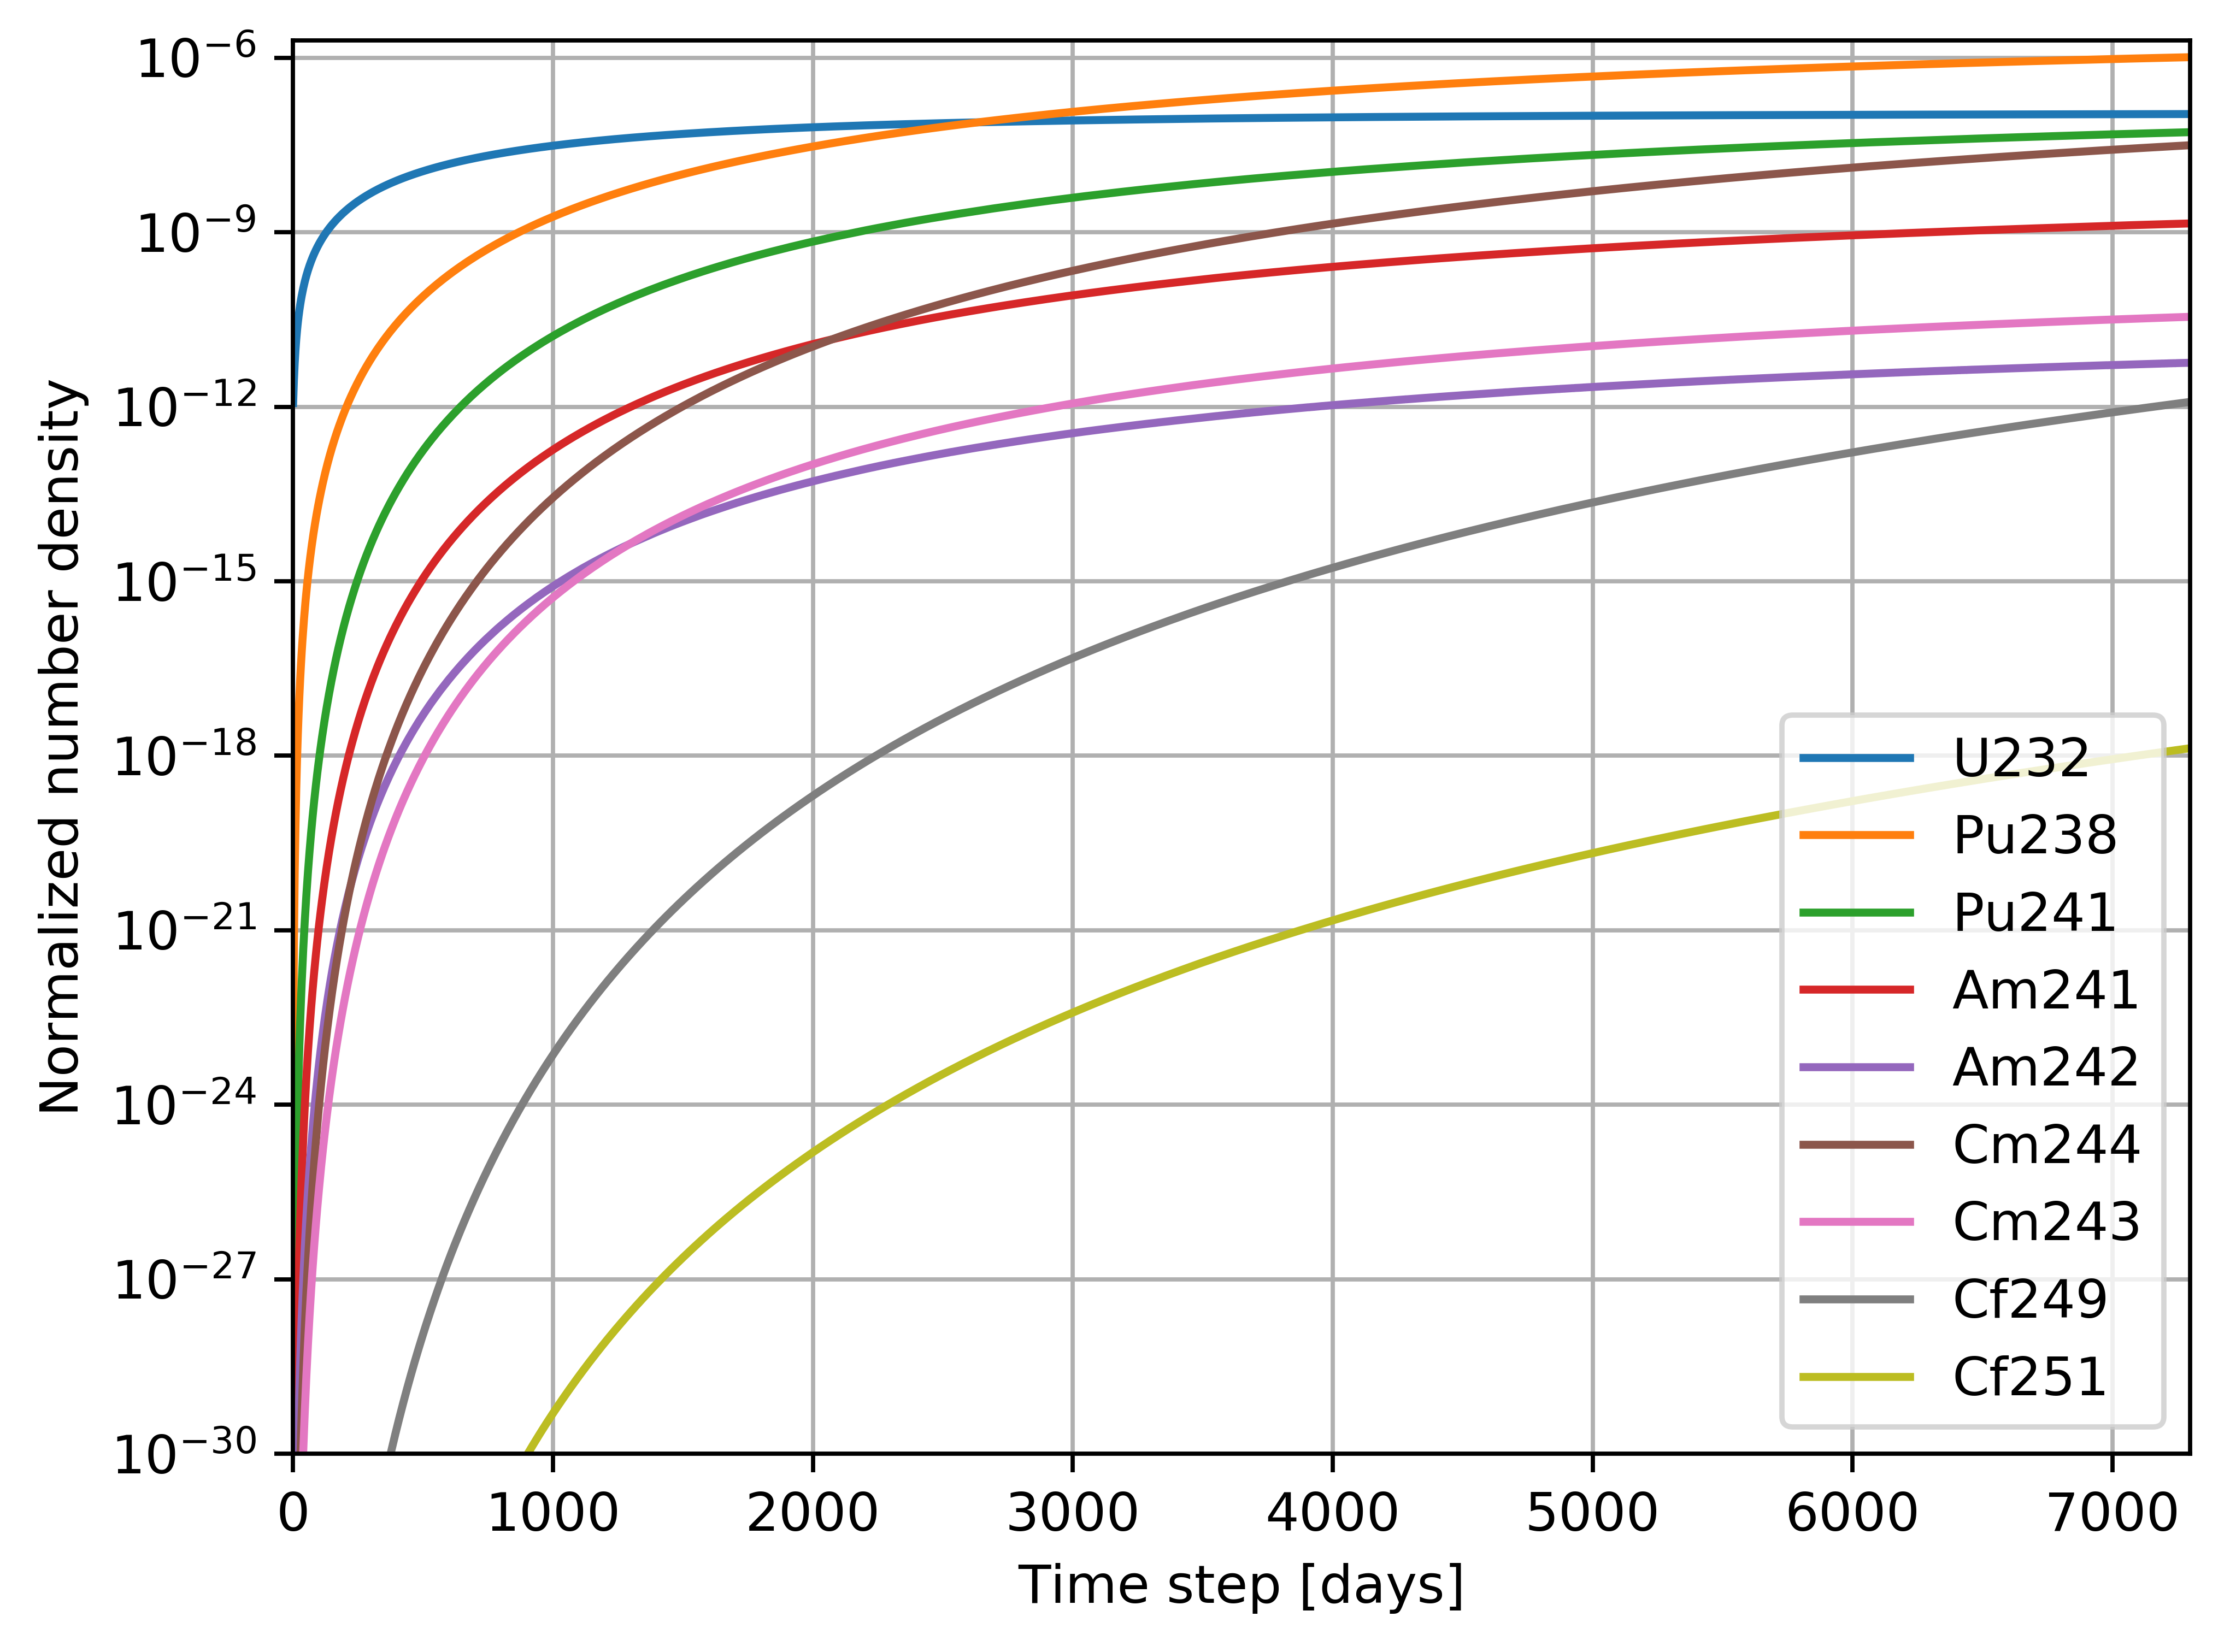
\includegraphics[height=0.75\textwidth]{./images/fissile_short.png}
               \end{figure}
    \column[t]{6cm}
               \begin{figure}[t]
                \vspace*{-0.1in}
                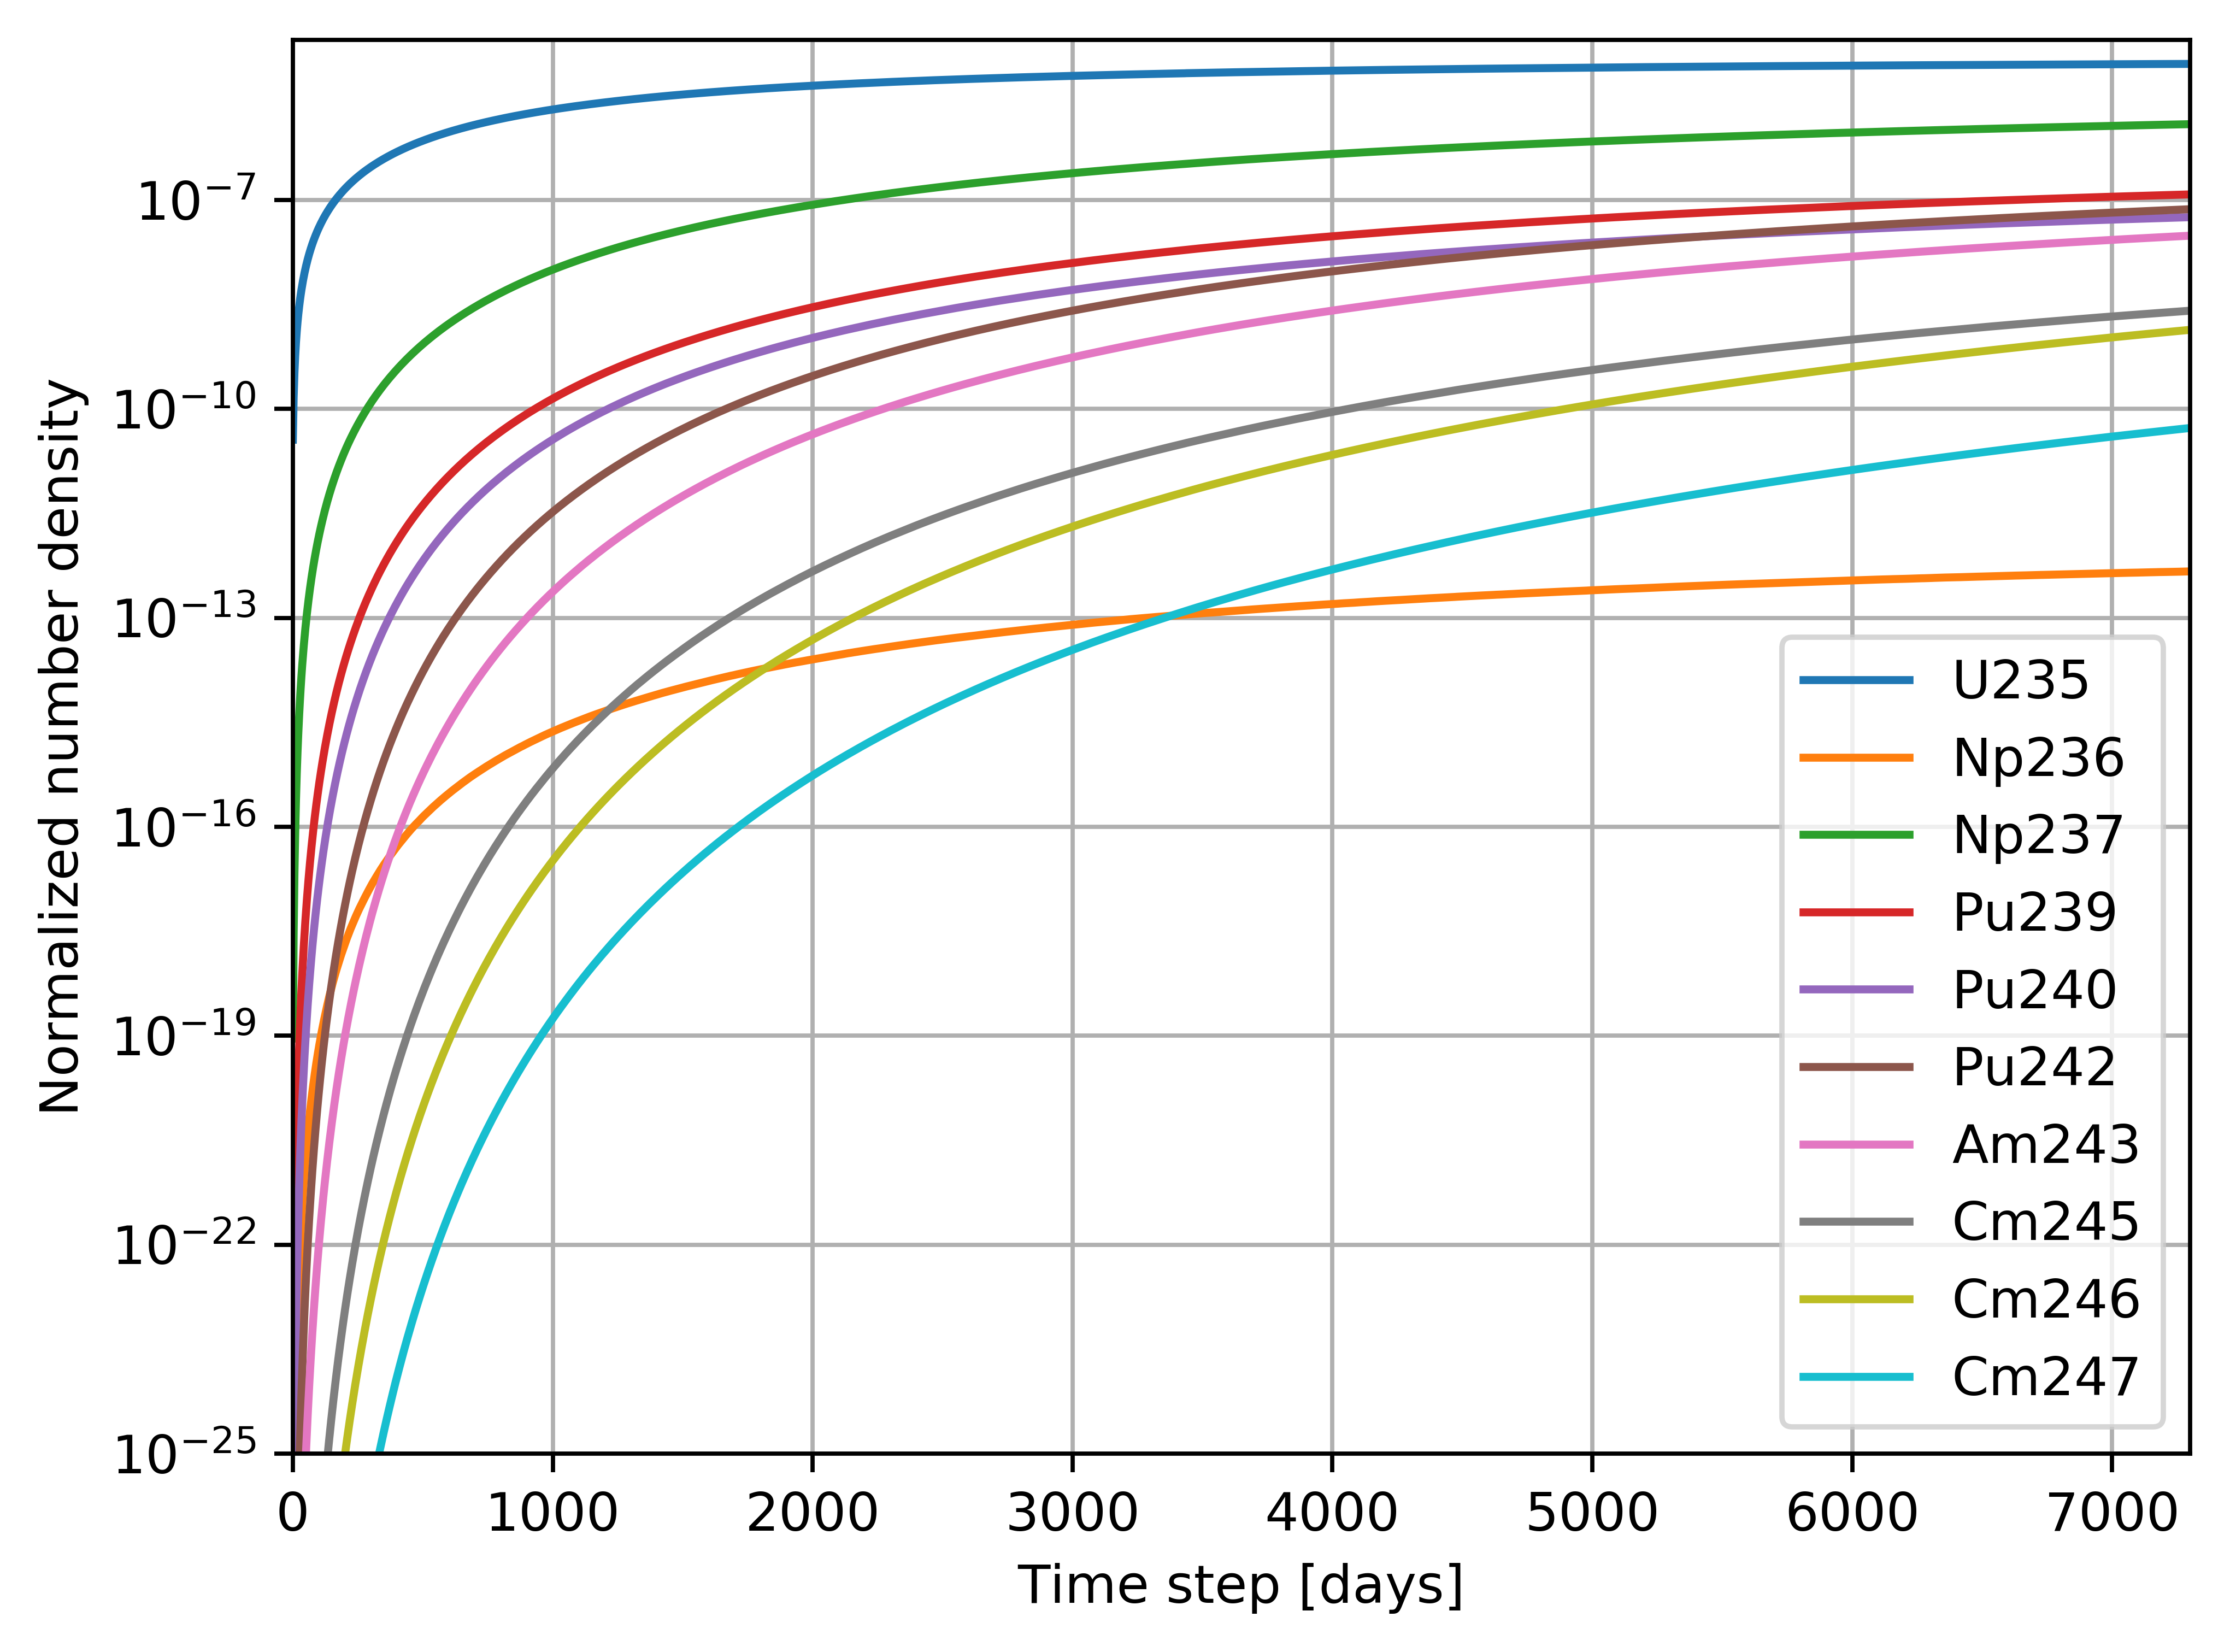
\includegraphics[height=0.75\textwidth]{./images/fissile_long.png}
               \end{figure}
    \end{columns}              
\end{frame}

\begin{frame}
  \frametitle{\gls{MSBR} plain view}
               \begin{figure}[t]
                \vspace*{-0.1in}
                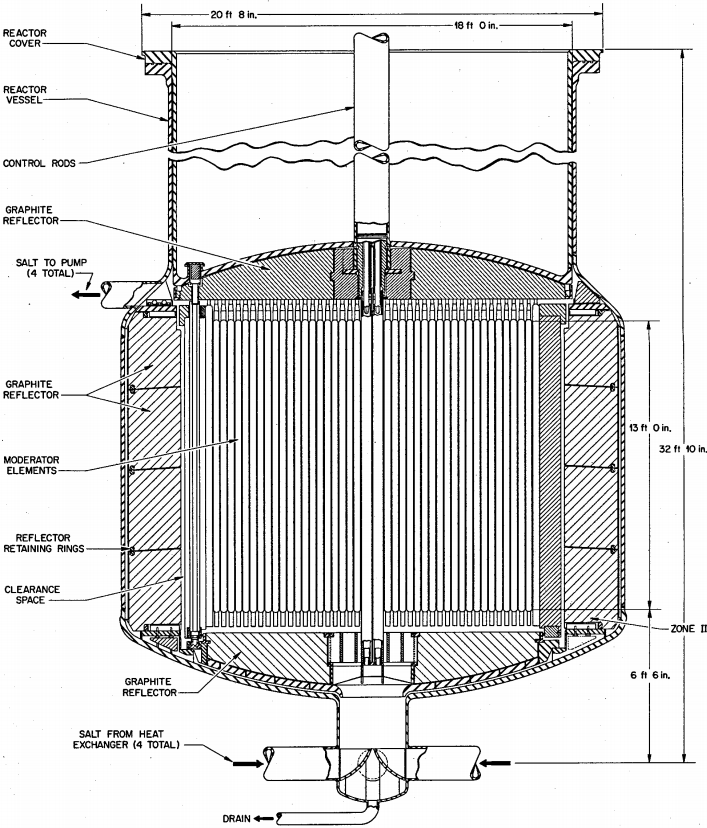
\includegraphics[height=0.75\textwidth]{./images/msbr_plain.png}
               \end{figure}
              
\end{frame}


\end{document}
